% Options for packages loaded elsewhere
\PassOptionsToPackage{unicode}{hyperref}
\PassOptionsToPackage{hyphens}{url}
%
\documentclass[
]{book}
\usepackage{amsmath,amssymb}
\usepackage{lmodern}
\usepackage{ifxetex,ifluatex}
\ifnum 0\ifxetex 1\fi\ifluatex 1\fi=0 % if pdftex
  \usepackage[T1]{fontenc}
  \usepackage[utf8]{inputenc}
  \usepackage{textcomp} % provide euro and other symbols
\else % if luatex or xetex
  \usepackage{unicode-math}
  \defaultfontfeatures{Scale=MatchLowercase}
  \defaultfontfeatures[\rmfamily]{Ligatures=TeX,Scale=1}
\fi
% Use upquote if available, for straight quotes in verbatim environments
\IfFileExists{upquote.sty}{\usepackage{upquote}}{}
\IfFileExists{microtype.sty}{% use microtype if available
  \usepackage[]{microtype}
  \UseMicrotypeSet[protrusion]{basicmath} % disable protrusion for tt fonts
}{}
\makeatletter
\@ifundefined{KOMAClassName}{% if non-KOMA class
  \IfFileExists{parskip.sty}{%
    \usepackage{parskip}
  }{% else
    \setlength{\parindent}{0pt}
    \setlength{\parskip}{6pt plus 2pt minus 1pt}}
}{% if KOMA class
  \KOMAoptions{parskip=half}}
\makeatother
\usepackage{xcolor}
\IfFileExists{xurl.sty}{\usepackage{xurl}}{} % add URL line breaks if available
\IfFileExists{bookmark.sty}{\usepackage{bookmark}}{\usepackage{hyperref}}
\hypersetup{
  pdftitle={ENG 792 - Análise e visualização de dados com R (RStudio)},
  pdfauthor={Jackson Rodrigues},
  hidelinks,
  pdfcreator={LaTeX via pandoc}}
\urlstyle{same} % disable monospaced font for URLs
\usepackage{color}
\usepackage{fancyvrb}
\newcommand{\VerbBar}{|}
\newcommand{\VERB}{\Verb[commandchars=\\\{\}]}
\DefineVerbatimEnvironment{Highlighting}{Verbatim}{commandchars=\\\{\}}
% Add ',fontsize=\small' for more characters per line
\usepackage{framed}
\definecolor{shadecolor}{RGB}{248,248,248}
\newenvironment{Shaded}{\begin{snugshade}}{\end{snugshade}}
\newcommand{\AlertTok}[1]{\textcolor[rgb]{0.94,0.16,0.16}{#1}}
\newcommand{\AnnotationTok}[1]{\textcolor[rgb]{0.56,0.35,0.01}{\textbf{\textit{#1}}}}
\newcommand{\AttributeTok}[1]{\textcolor[rgb]{0.77,0.63,0.00}{#1}}
\newcommand{\BaseNTok}[1]{\textcolor[rgb]{0.00,0.00,0.81}{#1}}
\newcommand{\BuiltInTok}[1]{#1}
\newcommand{\CharTok}[1]{\textcolor[rgb]{0.31,0.60,0.02}{#1}}
\newcommand{\CommentTok}[1]{\textcolor[rgb]{0.56,0.35,0.01}{\textit{#1}}}
\newcommand{\CommentVarTok}[1]{\textcolor[rgb]{0.56,0.35,0.01}{\textbf{\textit{#1}}}}
\newcommand{\ConstantTok}[1]{\textcolor[rgb]{0.00,0.00,0.00}{#1}}
\newcommand{\ControlFlowTok}[1]{\textcolor[rgb]{0.13,0.29,0.53}{\textbf{#1}}}
\newcommand{\DataTypeTok}[1]{\textcolor[rgb]{0.13,0.29,0.53}{#1}}
\newcommand{\DecValTok}[1]{\textcolor[rgb]{0.00,0.00,0.81}{#1}}
\newcommand{\DocumentationTok}[1]{\textcolor[rgb]{0.56,0.35,0.01}{\textbf{\textit{#1}}}}
\newcommand{\ErrorTok}[1]{\textcolor[rgb]{0.64,0.00,0.00}{\textbf{#1}}}
\newcommand{\ExtensionTok}[1]{#1}
\newcommand{\FloatTok}[1]{\textcolor[rgb]{0.00,0.00,0.81}{#1}}
\newcommand{\FunctionTok}[1]{\textcolor[rgb]{0.00,0.00,0.00}{#1}}
\newcommand{\ImportTok}[1]{#1}
\newcommand{\InformationTok}[1]{\textcolor[rgb]{0.56,0.35,0.01}{\textbf{\textit{#1}}}}
\newcommand{\KeywordTok}[1]{\textcolor[rgb]{0.13,0.29,0.53}{\textbf{#1}}}
\newcommand{\NormalTok}[1]{#1}
\newcommand{\OperatorTok}[1]{\textcolor[rgb]{0.81,0.36,0.00}{\textbf{#1}}}
\newcommand{\OtherTok}[1]{\textcolor[rgb]{0.56,0.35,0.01}{#1}}
\newcommand{\PreprocessorTok}[1]{\textcolor[rgb]{0.56,0.35,0.01}{\textit{#1}}}
\newcommand{\RegionMarkerTok}[1]{#1}
\newcommand{\SpecialCharTok}[1]{\textcolor[rgb]{0.00,0.00,0.00}{#1}}
\newcommand{\SpecialStringTok}[1]{\textcolor[rgb]{0.31,0.60,0.02}{#1}}
\newcommand{\StringTok}[1]{\textcolor[rgb]{0.31,0.60,0.02}{#1}}
\newcommand{\VariableTok}[1]{\textcolor[rgb]{0.00,0.00,0.00}{#1}}
\newcommand{\VerbatimStringTok}[1]{\textcolor[rgb]{0.31,0.60,0.02}{#1}}
\newcommand{\WarningTok}[1]{\textcolor[rgb]{0.56,0.35,0.01}{\textbf{\textit{#1}}}}
\usepackage{longtable,booktabs,array}
\usepackage{calc} % for calculating minipage widths
% Correct order of tables after \paragraph or \subparagraph
\usepackage{etoolbox}
\makeatletter
\patchcmd\longtable{\par}{\if@noskipsec\mbox{}\fi\par}{}{}
\makeatother
% Allow footnotes in longtable head/foot
\IfFileExists{footnotehyper.sty}{\usepackage{footnotehyper}}{\usepackage{footnote}}
\makesavenoteenv{longtable}
\usepackage{graphicx}
\makeatletter
\def\maxwidth{\ifdim\Gin@nat@width>\linewidth\linewidth\else\Gin@nat@width\fi}
\def\maxheight{\ifdim\Gin@nat@height>\textheight\textheight\else\Gin@nat@height\fi}
\makeatother
% Scale images if necessary, so that they will not overflow the page
% margins by default, and it is still possible to overwrite the defaults
% using explicit options in \includegraphics[width, height, ...]{}
\setkeys{Gin}{width=\maxwidth,height=\maxheight,keepaspectratio}
% Set default figure placement to htbp
\makeatletter
\def\fps@figure{htbp}
\makeatother
\usepackage[normalem]{ulem}
% Avoid problems with \sout in headers with hyperref
\pdfstringdefDisableCommands{\renewcommand{\sout}{}}
\setlength{\emergencystretch}{3em} % prevent overfull lines
\providecommand{\tightlist}{%
  \setlength{\itemsep}{0pt}\setlength{\parskip}{0pt}}
\setcounter{secnumdepth}{5}
\usepackage{booktabs}
\usepackage{booktabs}
\usepackage{longtable}
\usepackage{array}
\usepackage{multirow}
\usepackage{wrapfig}
\usepackage{float}
\usepackage{colortbl}
\usepackage{pdflscape}
\usepackage{tabu}
\usepackage{threeparttable}
\usepackage{threeparttablex}
\usepackage[normalem]{ulem}
\usepackage{makecell}
\usepackage{xcolor}
\ifluatex
  \usepackage{selnolig}  % disable illegal ligatures
\fi
\usepackage[]{natbib}
\bibliographystyle{plainnat}

\title{ENG 792 - Análise e visualização de dados com R (RStudio)}
\author{Jackson Rodrigues}
\date{2021-08-16}

\begin{document}
\maketitle

{
\setcounter{tocdepth}{1}
\tableofcontents
}
\hypertarget{apresentauxe7uxe3o}{%
\chapter{Apresentação}\label{apresentauxe7uxe3o}}

\hypertarget{hello-world---sejam-bem-vindos}{%
\section{Hello World! - Sejam Bem Vindos!}\label{hello-world---sejam-bem-vindos}}

Assista este conteúdo em \textbf{Cap 1 - Hello World! - Sejam Bem Vindos!} no \href{https://www2.cead.ufv.br/sistemas/pvanet/geral/login.php}{PVANet}.


\includegraphics[width=0.5\textwidth,height=0.5\textheight]{J:/ENG 792/ENG_792-AVDR/ENG.792-AVDR/Cap_1_ET.jpg}

Este é o material para os alunos matriculados na disciplina \textbf{ENG 792 - Análise e Visualização de dados com R (RStudio)} ofertada pelo programa de pós-graduação em Meteorologia Aplicada da Universidade Federal de Viçosa (UFV).

Este curso foi criado e é ministrado por Jackson Rodrigues, professor da Universidade Federal Fluminense (UFF), mas também professor no programa de pós-graduação em Meteorologia Aplicada do Departamento de Engenharia Agrícola (DEA) da Universidade Federal de Viçosa (UFV).

Este curso foi construído pensando em minha saga para aprender algo utilizando o R em meu doutorado. Foi bastante dolorido, principalmente no começo quando eu nunca havia tido contato com a liguagem, na verdade, sabia quase nada em programação.

Desta forma, o público alvo é aquele que tem conhecimento \textbf{zero} sobre o assunto. Mas se você já sabe algo em qualquer nível, seja bem vindo também! Podemos aprender juntos, você ensina o que você sabe e eu ensino o que eu sei.

A ideia principal deste curso é que o(a) aluno(a) que nada sabe de \textbf{R} seja exposto(a) a grande quantidade de conceitos e métodos para que o ``gelo'' seja quebrado e possa se virar sozinho ao término do curso. Desta forma, não é um curso de estatística, não é um curso de produção gráfica nem um curso produção de conteúdo (eg. modelagem), mas um curso de exposição, quase um ``\emph{how to}''. Vamos levantar demandas do dia a dia e tentar resolver os problemas comuns enfrentados pelo estudante na condução de suas análises.

Eventualmente algum especialista será convidado para dar uma aula, bater um papo, fazer uma apresentação e etc sobre um assunto específico.

O R é uma ferramenta espetacular para análise e produção de dados, bem como produção gráfica! Vamos começar devagar e ao poucos vocês vão se tornando autossuficientes.
Muitas dúvidas surgem em fóruns, grupos e tanto outros canais de comunicação da comunidade de usuários de R.

Muitas vezes surgem perguntas como:\textbf{"Tem como fazer isso no R?} A resposta imediada, devido à sua versatilidade, é: \textbf{A pergunta não é ``se tem jeito'', mas ``como fazer''}.

Vamos dar uma passeio por muitas coisas legais que o \textbf{R} pode fazer e que vão ajudar a tornar sua vida bem melhor. Com tempo ganho na otimização das suas tarefas por utilização do \textbf{R} sobrará tempo para você escrever um paper a mais na pós-graduação, dormir no final de semana sem culpa, tomar uma cerveja na sexta com a turma e ir ao culto domingo sem pedidos.

Vamos fazer tudo isso nos divertindo. É legal! Vocês verão. Por isso não se procupem comigo (professor), será muito pior para mim por ter que corrigir trabalhos enquanto vocês produzem mais um paper, dormem, tomam um cerveja com a turma e/ou rezam como foi na véspera de natal de 2020 quando estava corrigindo trabalhos.

\begin{figure}
\hypertarget{id}{%
\centering
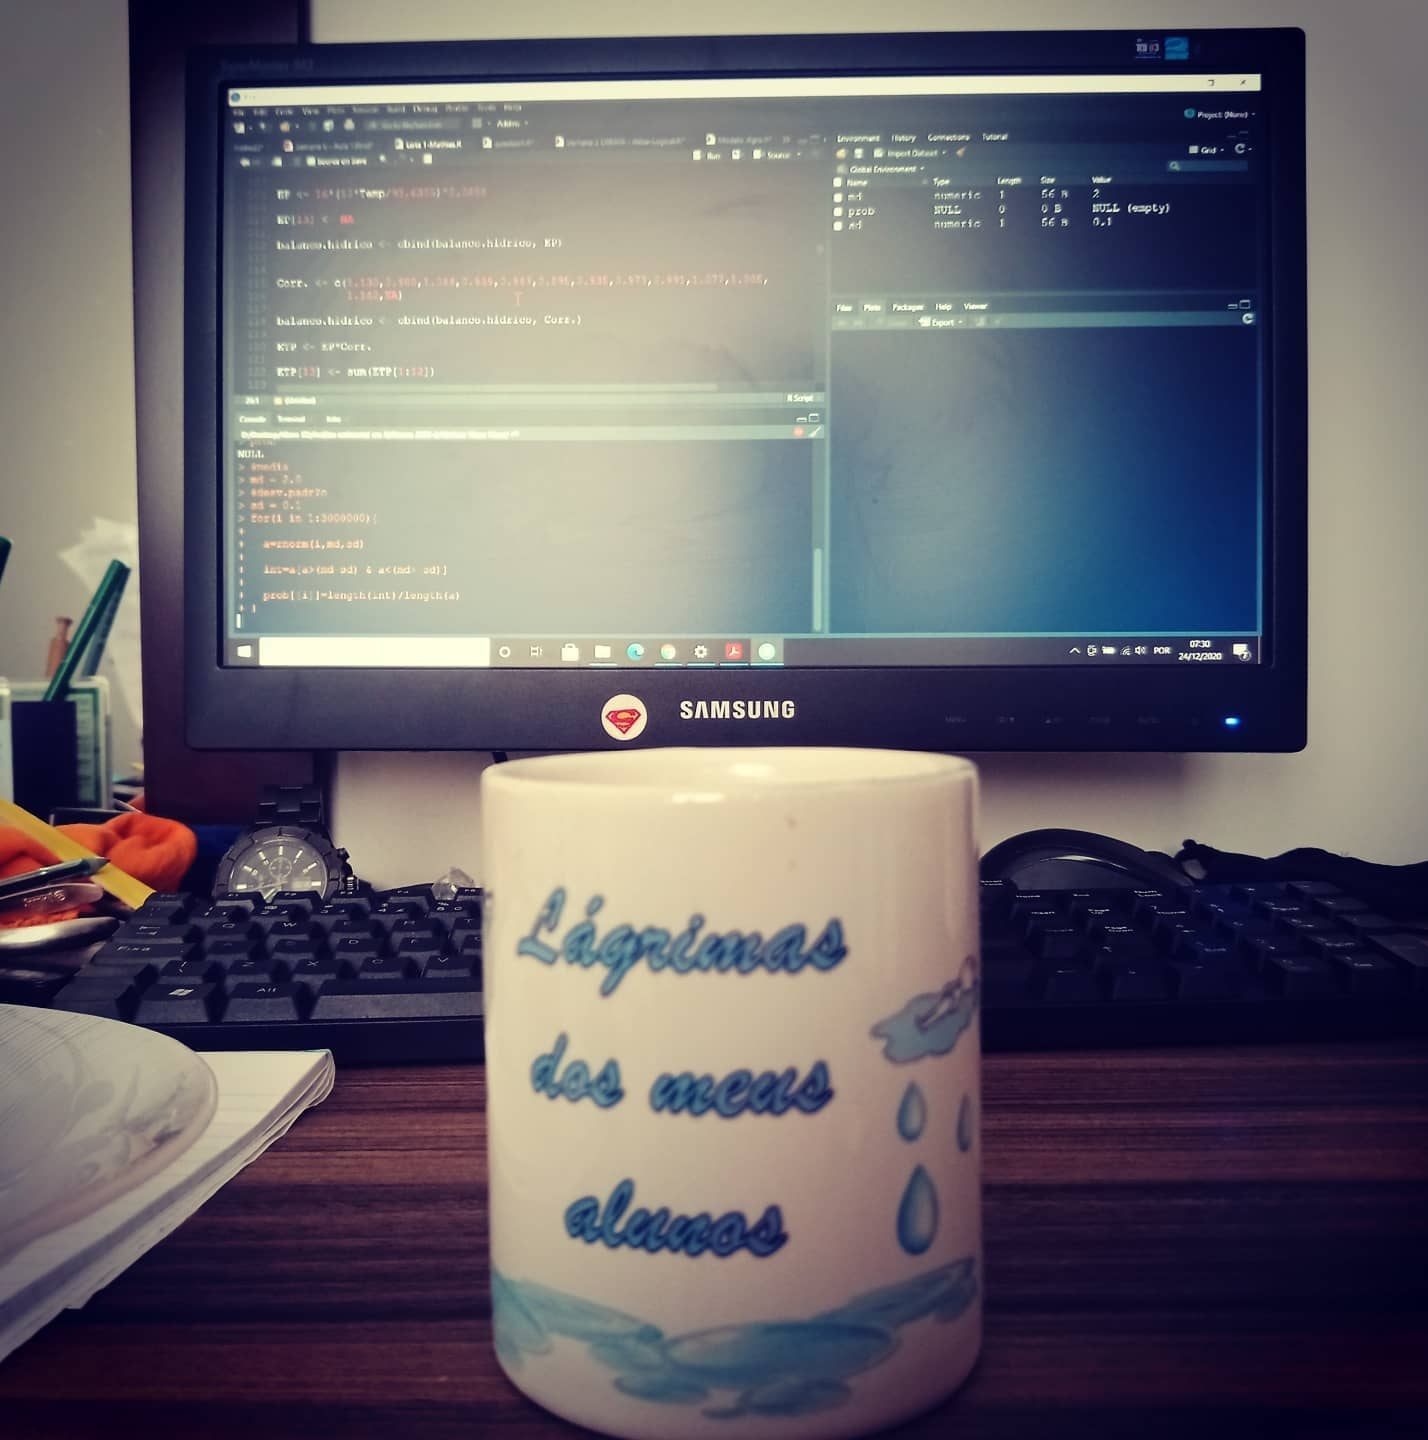
\includegraphics[width=0.7\textwidth,height=0.7\textheight]{J:/ENG 792/ENG_792-AVDR/ENG.792-AVDR/Cap_1_Vespera_de_Natal.jpg}
\caption{Véspera de Natal 2020}\label{id}
}
\end{figure}

\href{https://www.youtube.com/watch?v=N8E4s8yAoX4\&ab_channel=MassacrationOficial}{Let's ride to Metal Land!}

Não se sintam pressionados ou intimidados, façam as perguntas que quiserem. Eu também não sei tudo, o R é uma ferramenta que está em constante desenvolvimento tornando impossível acompanhar cada novidade. Caso eu não saiba uma resposta não tenho problemas em dizer que não sei, mas vou me esforçar para buscar a resposta.

Por isso:

\begin{itemize}
\item
  Vamos aprender e tentar nos divertir;
\item
  Pensei nesse curso como uma forma de lutar contra a ``dor'' que senti quando comecei a trabalhar no R sozinho;
\item
  Então sou um usuário e não um programador;
\item
  A verdade é que o R tem uma curva de aprendizado muito íngreme que uma vez vencido o primeiro obstáculo as coisas deslancham;
\item
  Vamos trabalhar de maneira que esse curso atenda superficialmente suas demandas e que te habilitem a se virarem sozinhos;
\item
  Então vamos seguir passo-a-passo para um aprendizado gradual com vários exemplos;
\item
  Tudo que você aprender em determinando momento não será descartado, você deverá guardar aquele conhecimento para utilização em próximo trabalho ou tarefa;
\item
  Ou ainda, este conhecimento inicial será utilizado para sedimentar o caminho para um próximo passo;
\item
  Aplicar o máximo possível nosso conhecimento a problemas reais, do mundo real.
\end{itemize}

Para finalizar gostaria de deixar algumas coisas claras.

\begin{itemize}
\item
  Este curso conta com vasto material encontrado em artigos, livros, blogs especializados, grupos de discussões e etc. Desta forma, caso encontre por aí algo que ofertei em aula não precisa me chamar de picareta. Provavelmente foi tirado de lá mesmo.
\item
  O curso funciona como um \textbf{\emph{How to}}. Não teremos tempo de nos aprofundar nas teorias dos assuntos aqui apresentados (nem é a intenção), por isso, vou mostrar o \textbf{``que é''}, \textbf{``como usar''} e \textbf{``como fazer''}.
\item
  Ao término de cada aula será mostrada uma bibliografia básica sobre o conteúdo. Como são conteúdos diversificados, acho melhor separar as bibliografias por aula.
\end{itemize}

\hypertarget{sobre}{%
\subsection{Sobre}\label{sobre}}

Este é um material de apoio compilado e criado para os alunos da disciplina \textbf{ENG 792 - Análise e visualização de dados com R (RStudio)}.

Importante mencionar que o conteúdo aqui apresentado é um compilado de vários anos de materiais estudados disponíveis \emph{online} ou em livros e artigos especialzados. Desta forma, caso identifique algum conteúdo apresentado aqui que não esteja devidamente referenciado fique à vontade para solicitar os devidos créditos aos autores originais. Não tenho a intenção de ter crédito que não é meu.

\hypertarget{utilizauxe7uxe3o}{%
\subsection{Utilização}\label{utilizauxe7uxe3o}}

Cada capítulo é referente ao conteúdo de mais ou menos uma semana de curso. Cada semama trata de um assunto diferente e complementar ao conteúdo da semana anterior.
Desta forma, fique livre para ir e vir no conteúdo caso algo não esteja claro o suficiente.

\begin{itemize}
\tightlist
\item
  Teremos aulas gravadas e aulas síncronas através de alguma plataforma.\\
\item
  Apenas os alunos matriculados na disciplina terão acesso ao conteúdo gravado.\\
\item
  A distribuição e/ou compartilhamento do conteúdo gravado por qualquer meio é proibido.
\end{itemize}

\hypertarget{cuxf3digos-e-dados}{%
\subsection{Códigos e Dados}\label{cuxf3digos-e-dados}}

Todo o material necessário para acompanhar a disciplina será oferecido via \href{https://github.com/Jacksonmrod/ENG-792}{github}. Os códigos com alguma explicação neste material online (explicação completa nas aulas) e os dados onde forem possíveis de serem armazenados.

\hypertarget{cronograma-de-aulas}{%
\subsection{Cronograma de aulas}\label{cronograma-de-aulas}}

As aulas serão ofertadas por material gravado e presencial às quintas e sextas entre 14:00 e 15:30.

\begin{longtable}[]{@{}
  >{\centering\arraybackslash}p{(\columnwidth - 2\tabcolsep) * \real{0.12}}
  >{\centering\arraybackslash}p{(\columnwidth - 2\tabcolsep) * \real{0.88}}@{}}
\toprule
Semana & Conteúdo \\
\midrule
\endhead
1.1 & Apresentação do Conteúdo e Instalação do R \\
1.2 & Funcionamento do R, tipo e estrutura dos objetos \\
2.1 & Manipulação de dados 1 \\
2.2 & Manipulação de dados 2, testes lógicos e simbolos, condicionais e interações \\
3.1 & Pacotes e Funções \\
3.2 & Entrando/Importando dados. definição de diretórios \\
4.1 & Produção gráfica com Rbase \\
4.2 & Produção gráfica com ggplot 2 \\
5.1 & Elementos de estatística básica 1 (Est. Descritiva, Med. Tend. Central, Medi. de variabilidade) \\
5.2 & Elementos de estatítica básica 2 (Dife. Entre médias, T-Student, Teste F, Testes de normalidade) \\
6.1 & Elementos de estatítica básica 3 (ANOVA, delineamento, comparaçõe múltiplas, Regressão, Resíduos, Homocedasticidade, Normalidade dos resíduos, regressão múltipla, superfície de resposta) \\
7.1 & Análise Multivariada (Análise de agrupamento, medidas de (dis)similaridade, métodos de conexão, número de clusters, produção de dendogramas, árvores de decisão) \\
7.2 & Métodos de Ordenação (Ana. Componentes Principais, Análise Canônica, Análise de fatores, Análise de Mahalanobis) \\
8 - 15 & Será preenchido em breve \\
\bottomrule
\end{longtable}

\hypertarget{muxe9todos-de-avaliauxe7uxe3o}{%
\subsection{Métodos de avaliação}\label{muxe9todos-de-avaliauxe7uxe3o}}

\begin{itemize}
\tightlist
\item
  Faremos pelo menos 3 listas de exercícios distribuídas pelo semestre.\\
\item
  O trabalho final será a confecção de um atrabalho autoral com o conteúdo do curso que poderá ser feito em grupo (isso será definido ainda em conversa com vocês). Este trabalho será apresentado na forma de seminário ao término do curso.
\end{itemize}

\hypertarget{vamos-ao-que-interesa}{%
\chapter{Vamos ao que interesa}\label{vamos-ao-que-interesa}}

\hypertarget{conhecendo-o-r}{%
\section{Conhecendo o R}\label{conhecendo-o-r}}

\hypertarget{o-que-uxe9-o-r}{%
\subsection{O que é o R?}\label{o-que-uxe9-o-r}}

É uma linguagem de programação voltada para resolução de problemas estatísticos, tratamento e visualização de dados.

Para \citet{RogerPeng2020RPro} essa resposta é simples, ``\emph{R é um dialeto do S}''.

De acordo com \citet{perlin2018processamento} \emph{O código base do R foi inicialmente criado no laboratório da Bell/ AT\& T por John Chambers e seus colegas, com base na linguagem S. Esse código foi reaproveitado por dois acadêmicos, Ross Ihaka e Robert Gentleman, resultando na plataforma de programação que temos hoje. Para os curiosos, o nome R foi escolhido devido ao compartilhamento da primeira letra do nome de seus criadores.}


\includegraphics[width=0.7\textwidth,height=0.7\textheight]{J:/ENG 792/ENG_792-AVDR/ENG.792-AVDR/Cap_1_Ross_Robert R.jpg}

O R está em constante desenvolvimento por um grupo chamado \href{https://www.r-project.org/}{R Team Core} e conta com colaboração gratuita de centenas de milhares de usuários e desenvolvedores ao redor do mundo.
Por isso, atualmente o R é utilizado por diversas áreas do conhecimento variando das ciências humanas até exatas, naquelas ciências que poderíamos imaginar pouco ou nada relacionadas. Por isso não se limite a procurar informações apenas no seu nicho, abra sua mente e busque aprender de outras ciências também. Eu, particularmente, busco muita coisa na econometria. Embora presente em todo tipo de livro sobre R, esta citação acima (\citet{perlin2018processamento}) é de um livro de econometria. Veremos mais conteúdos desse material em breve.

R é um software livre de análise de dados (não só estatística) que funciona em diversos sistemas operacionais: GNU Linux, MicrosoftWindows, Mac OS X e outros.

O aprendizado do R é difícil no início devido à necessidade de se adaptar à sua lógica de funcionamento, se acostumar com a estrutura dos seus documentos de ajuda e memorizar alguns comandos básicos.

\begin{Shaded}
\begin{Highlighting}[]
\NormalTok{eq }\OtherTok{=} \ControlFlowTok{function}\NormalTok{(x)\{x}\SpecialCharTok{*}\NormalTok{x\}}
\FunctionTok{plot}\NormalTok{(}\FunctionTok{eq}\NormalTok{(}\DecValTok{1}\SpecialCharTok{:}\DecValTok{1000}\NormalTok{), }\AttributeTok{type=}\StringTok{"l"}\NormalTok{,}\AttributeTok{lwd=}\DecValTok{3}\NormalTok{,}\AttributeTok{col=}\StringTok{"red"}\NormalTok{, }\AttributeTok{xaxt=}\StringTok{"n"}\NormalTok{, }\AttributeTok{yaxt=}\StringTok{"n"}\NormalTok{, }\AttributeTok{xlab=}\StringTok{"Tempo"}\NormalTok{, }\AttributeTok{ylab=}\StringTok{"Aprendizado"}\NormalTok{, }\AttributeTok{main=}\StringTok{"Curva de Aprendizado"}\NormalTok{)}
\end{Highlighting}
\end{Shaded}

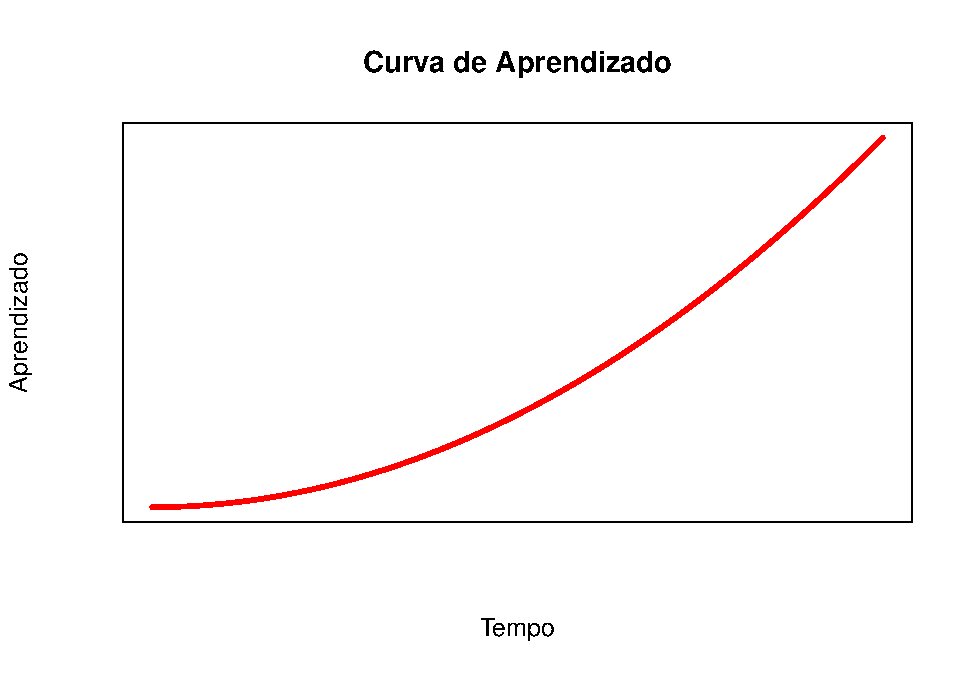
\includegraphics{ENG_792-AVDR_files/figure-latex/CurvaR-1.pdf}

É preciso bastante perseverança e motivação para aprender os comandos básicos, e disposição para ler as páginas de ajuda e os manuais.
Entretanto, depois de um certo tempo, ele possibilita que se trabalhe com grande produtividade e, o que é mais importante, eficácia e independência.

Leia também sobre o \href{https://www.r-bloggers.com/2021/07/the-myth-of-the-r-learning-curve/}{mito da curva de aprendizado do R}.

\hypertarget{instalauxe7uxe3o-do-r}{%
\subsection{Instalação do R}\label{instalauxe7uxe3o-do-r}}

O \textbf{R} é um software gratuito para análises estatísticas e além. Pode ser baixado de \href{https://www.r-project.org/}{The R Project for Statistical Computing}.

Clique em \textbf{download R}.\\
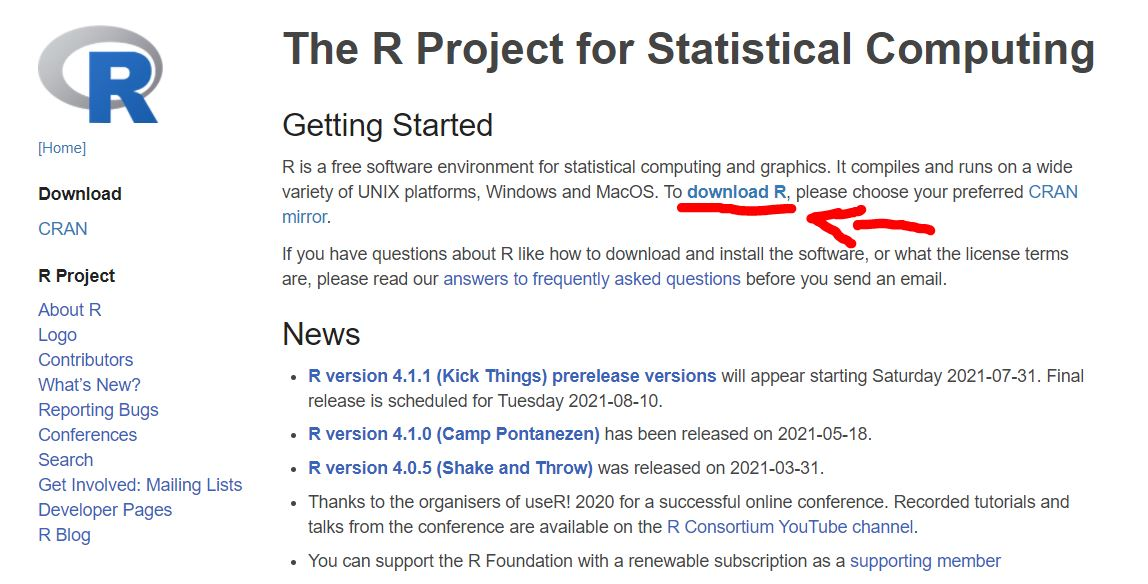
\includegraphics[width=0.9\textwidth,height=0.9\textheight]{J:/ENG 792/ENG_792-AVDR/ENG.792-AVDR/Cap_1_Pagina_R.jpg}

Escolha o \emph{``espelho''}.Escolha o mais próximo de você.\\

\includegraphics[width=0.9\textwidth,height=0.9\textheight]{J:/ENG 792/ENG_792-AVDR/ENG.792-AVDR/Cap_1_Pagina_R_MIrror.jpg}

Escolha o seu sistema operacional. Caso você seja usuário de windows clique em \textbf{Download R for Windows} em seguinda em \textbf{install R for the first time} e finalmente em \textbf{Download R 4.1.0 for Windows}. Veja que no momento que este tutorial foi feito a versão mais recente é a 4.1.0. No vídeo abaixo a versão é uma anterior, mas a lógica é a mesma.\\
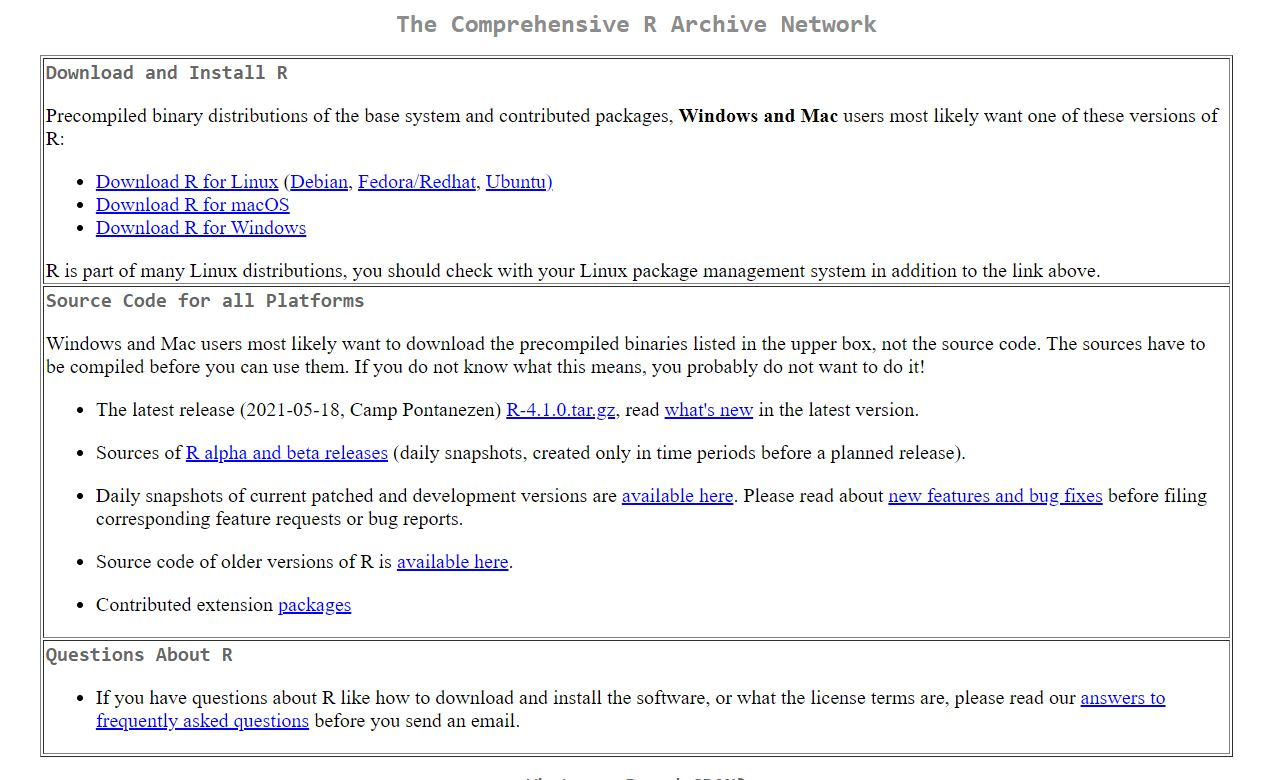
\includegraphics[width=0.9\textwidth,height=0.9\textheight]{J:/ENG 792/ENG_792-AVDR/ENG.792-AVDR/Cap_1_Pagina_R_sistema_operacional.jpg}

Assista este conteúdo em \textbf{Cap 1 - Instalação do R no Windows} no \href{https://www2.cead.ufv.br/sistemas/pvanet/geral/login.php}{PVANet}.

Eu não tenho um sistema operacional de cada para mostrar a instalação, por isso deixo este vídeo para \href{https://www.youtube.com/watch?v=np2-FIgzpTg\&ab_channel=AutoDeeDucks}{instalação no linux} e este para \href{https://www.youtube.com/watch?v=LanBozXJjOk\&ab_channel=DataSciencewithTom}{instalação no mac}. Caso você não consiga instalar me procure.

\hypertarget{primeiro-contato}{%
\subsection{Primeiro contato}\label{primeiro-contato}}

Assista este conteúdo em \textbf{Cap 1 - Primeiro contato} no \href{https://www2.cead.ufv.br/sistemas/pvanet/geral/login.php}{PVANet}.


\includegraphics[width=0.5\textwidth,height=0.5\textheight]{J:/ENG 792/ENG_792-AVDR/ENG.792-AVDR/Cap_1_ET-dedo.jpg}

Temos 1 arquivo \textbf{Cap\_1\_P2-Mispriced-Diamonds.csv} \href{https://www2.cead.ufv.br/sistemas/pvanet/geral/login.php}{PVANet} no PVANet com mais de 50.000 linhas referentes a transações de venda de diamantes dividida em 3 colunas \emph{clarity}, \emph{carat} e \emph{price}. Quanto mais claro mais caro, certo? Ou há sub ou super valorização? Vamos investigar se essa relação é verdadeira como sugerido em \href{https://ecapitaladvisors.com/blog/finding-mispriced-diamonds/}{ecapitaladvisors}.

Abaixo vamos apenas dar uma olhada no potencial de análise e produção gráfica do R. Não precisa se preocupar se não conseguir fazer tudo funcionar. Vamos aos poucos aprender cada comando apresentado.

\begin{Shaded}
\begin{Highlighting}[]
\NormalTok{mydata}\OtherTok{\textless{}{-}}\FunctionTok{read.csv}\NormalTok{(}\StringTok{"J:/ENG 792/ENG\_792{-}AVDR/ENG.792{-}AVDR/Cap\_1\_P2{-}Mispriced{-}Diamonds.csv"}\NormalTok{)}

\FunctionTok{library}\NormalTok{(}\StringTok{"ggplot2"}\NormalTok{)}
\FunctionTok{ggplot}\NormalTok{(}\AttributeTok{data=}\NormalTok{mydata, }\FunctionTok{aes}\NormalTok{(}\AttributeTok{x=}\NormalTok{carat, }\AttributeTok{y=}\NormalTok{price))}\SpecialCharTok{+} 
  \FunctionTok{geom\_point}\NormalTok{()}
\end{Highlighting}
\end{Shaded}

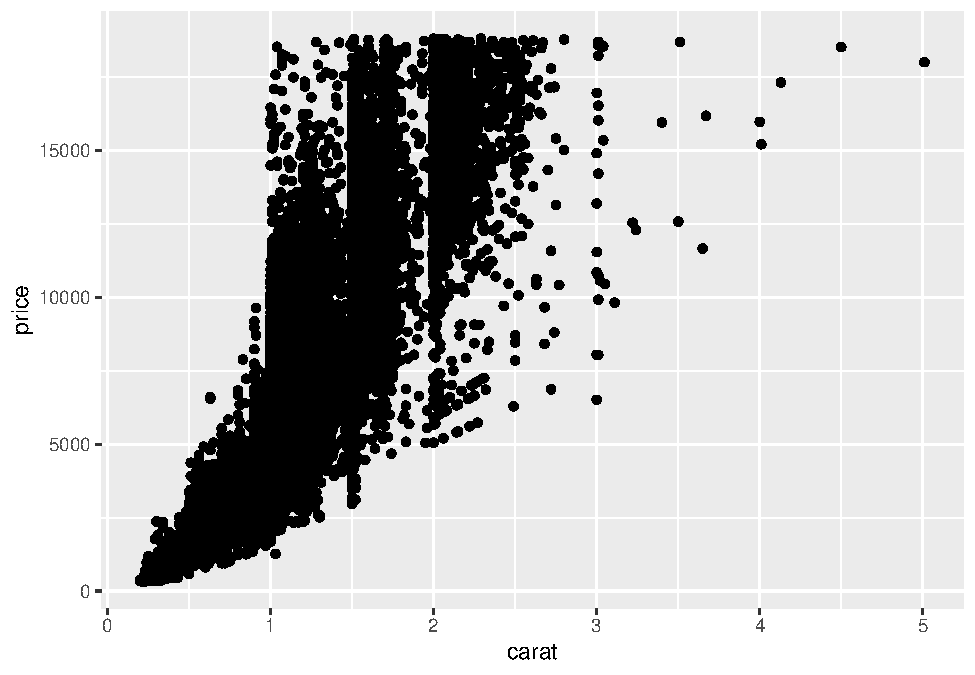
\includegraphics{ENG_792-AVDR_files/figure-latex/Exemplo_1-1.pdf}

Faz algum sentido. Mas está difícil de visualizar então vamos fazer um tratamento, vamos atribuir cores de acordo com a classificação do atributo \emph{clarity}.

\begin{Shaded}
\begin{Highlighting}[]
\FunctionTok{ggplot}\NormalTok{(}\AttributeTok{data=}\NormalTok{mydata, }\FunctionTok{aes}\NormalTok{(}\AttributeTok{x=}\NormalTok{carat, }\AttributeTok{y=}\NormalTok{price, }\AttributeTok{colour=}\NormalTok{clarity))}\SpecialCharTok{+} 
  \FunctionTok{geom\_point}\NormalTok{()}
\end{Highlighting}
\end{Shaded}

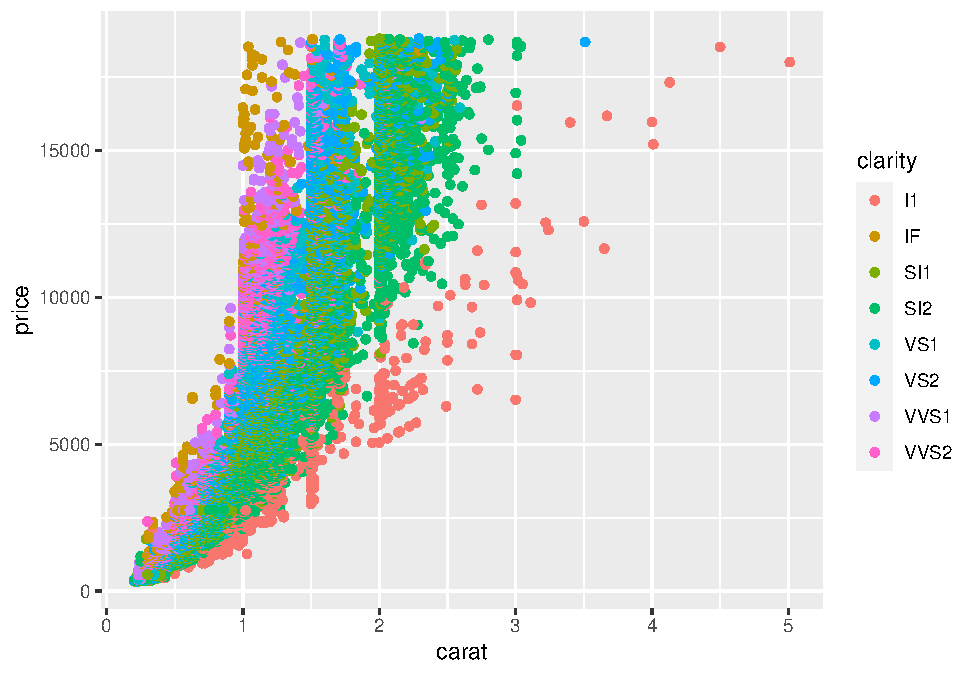
\includegraphics{ENG_792-AVDR_files/figure-latex/Exemplo_1.2-1.pdf}

Os pontos estão sobrepostos impossibilitando a visualização. Vamos mexer na transparência.

\begin{Shaded}
\begin{Highlighting}[]
\FunctionTok{ggplot}\NormalTok{(}\AttributeTok{data=}\NormalTok{mydata,}
       \FunctionTok{aes}\NormalTok{(}\AttributeTok{x=}\NormalTok{carat, }\AttributeTok{y=}\NormalTok{price, }\AttributeTok{colour=}\NormalTok{clarity))}\SpecialCharTok{+}
\FunctionTok{geom\_point}\NormalTok{(}\AttributeTok{alpha=}\FloatTok{0.1}\NormalTok{) }
\end{Highlighting}
\end{Shaded}

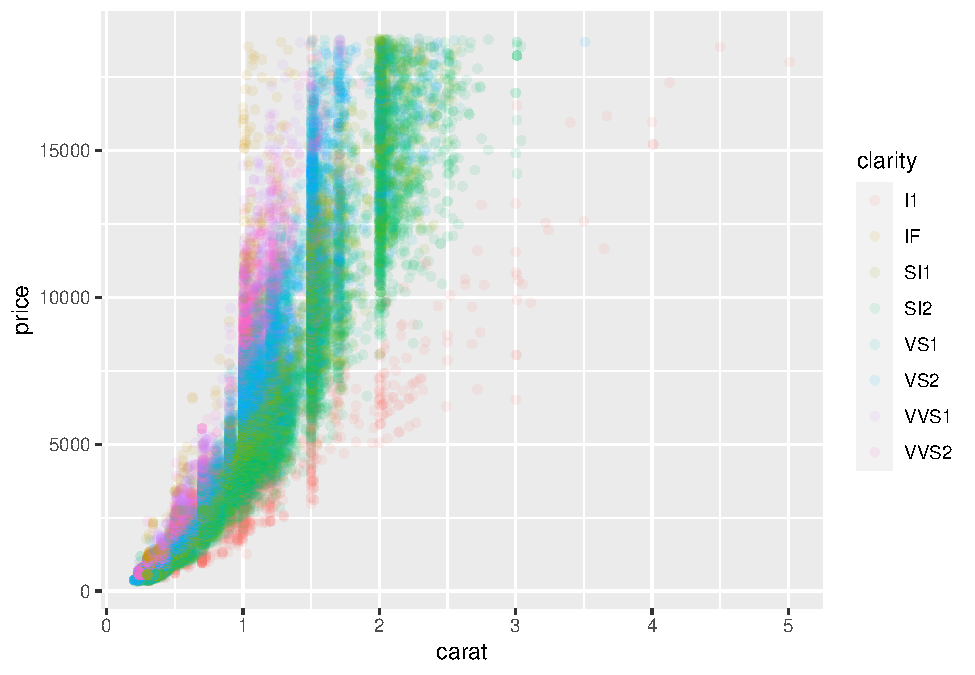
\includegraphics{ENG_792-AVDR_files/figure-latex/Exemplo_1.3-1.pdf}

Temos pontos que não são estatisticamente significantes à direita. Vamos nos livrar dos pontos não significativos, aqueles que são \emph{carat} menores que 2.5.

Vamos também adicionar algumas linhas através dos dados para avaliar o comportamento das variáveis em conjunto.

\textbf{brown} é a melhor claridade, vejam que temos mispricing onde as linhas se cruzam.

\begin{Shaded}
\begin{Highlighting}[]
\FunctionTok{ggplot}\NormalTok{(}\AttributeTok{data=}\NormalTok{mydata[mydata}\SpecialCharTok{$}\NormalTok{carat}\SpecialCharTok{\textless{}}\FloatTok{2.5}\NormalTok{,],}
       \FunctionTok{aes}\NormalTok{(}\AttributeTok{x=}\NormalTok{carat, }\AttributeTok{y=}\NormalTok{price, }\AttributeTok{colour=}\NormalTok{clarity))}\SpecialCharTok{+}
\FunctionTok{geom\_point}\NormalTok{(}\AttributeTok{alpha=}\FloatTok{0.1}\NormalTok{) }\SpecialCharTok{+}
  \FunctionTok{geom\_smooth}\NormalTok{()}
\end{Highlighting}
\end{Shaded}

\begin{verbatim}
## `geom_smooth()` using method = 'gam' and formula 'y ~ s(x, bs = "cs")'
\end{verbatim}

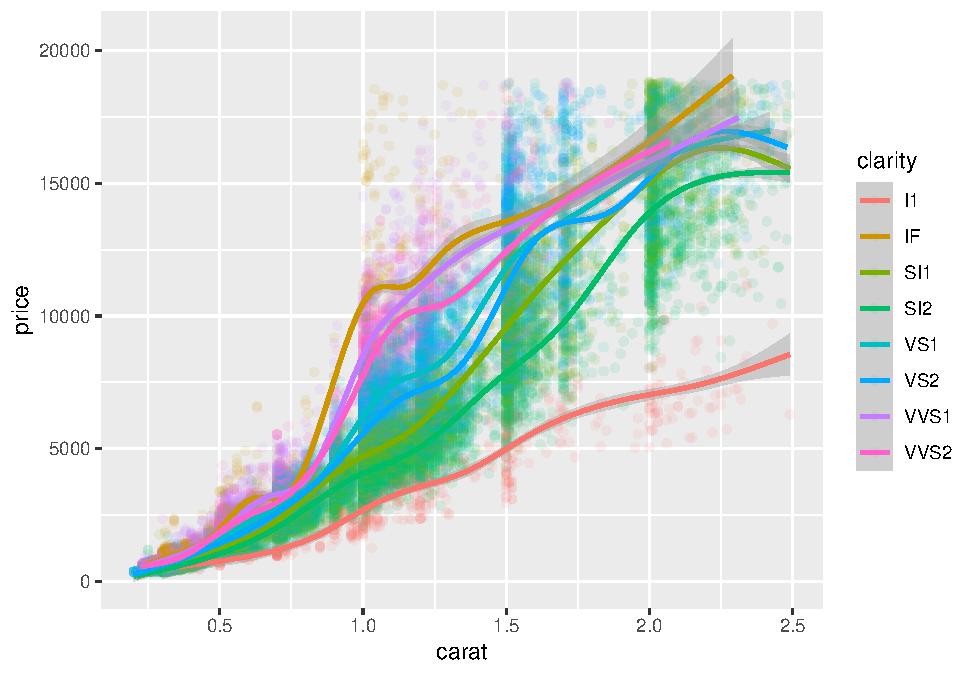
\includegraphics{ENG_792-AVDR_files/figure-latex/Exemplo_1.4-1.pdf}

\textbf{Vamos agora reproduzir um ourto exemplo muito legal do pacote \href{https://www.rayshader.com/}{rayshader}.}

Executando o código abaixo você produzirá uma Modelo Digital do Terreno em 3D em uma janela \textbf{pop up}.

\begin{Shaded}
\begin{Highlighting}[]
\FunctionTok{library}\NormalTok{(rayrender)}
\FunctionTok{library}\NormalTok{(rayshader)}
\FunctionTok{library}\NormalTok{(magick)}

\CommentTok{\#Vamos carregar o mapa com o pacote raster.}
\NormalTok{loadzip }\OtherTok{=} \FunctionTok{tempfile}\NormalTok{() }
\FunctionTok{download.file}\NormalTok{(}\StringTok{"https://tylermw.com/data/dem\_01.tif.zip"}\NormalTok{, loadzip)}
\NormalTok{localtif }\OtherTok{=}\NormalTok{ raster}\SpecialCharTok{::}\FunctionTok{raster}\NormalTok{(}\FunctionTok{unzip}\NormalTok{(loadzip, }\StringTok{"dem\_01.tif"}\NormalTok{))}
\FunctionTok{unlink}\NormalTok{(loadzip)}

\CommentTok{\# convertê{-}lo para matriz:}
\NormalTok{elmat }\OtherTok{=} \FunctionTok{raster\_to\_matrix}\NormalTok{(localtif)}

\CommentTok{\#Usar uma outra textura do rayshader}
\NormalTok{elmat }\SpecialCharTok{\%\textgreater{}\%}
  \FunctionTok{sphere\_shade}\NormalTok{(}\AttributeTok{texture =} \StringTok{"desert"}\NormalTok{) }\SpecialCharTok{\%\textgreater{}\%}
  \FunctionTok{add\_water}\NormalTok{(}\FunctionTok{detect\_water}\NormalTok{(elmat), }\AttributeTok{color =} \StringTok{"desert"}\NormalTok{) }\SpecialCharTok{\%\textgreater{}\%}
  \FunctionTok{plot\_3d}\NormalTok{(elmat, }\AttributeTok{zscale =} \DecValTok{10}\NormalTok{, }\AttributeTok{fov =} \DecValTok{0}\NormalTok{, }\AttributeTok{theta =} \DecValTok{60}\NormalTok{, }\AttributeTok{zoom =} \FloatTok{0.75}\NormalTok{, }\AttributeTok{phi =} \DecValTok{45}\NormalTok{, }\AttributeTok{windowsize =} \FunctionTok{c}\NormalTok{(}\DecValTok{1000}\NormalTok{, }\DecValTok{800}\NormalTok{))}
\end{Highlighting}
\end{Shaded}


\includegraphics{J:/ENG 792/ENG_792-AVDR/ENG.792-AVDR/Cap_1_rayshader.jpeg}

Agora vamos adicionar mais algumas infromações como escala e indicador de norte.

\begin{Shaded}
\begin{Highlighting}[]
\FunctionTok{render\_scalebar}\NormalTok{(}\AttributeTok{limits=}\FunctionTok{c}\NormalTok{(}\DecValTok{0}\NormalTok{, }\DecValTok{5}\NormalTok{, }\DecValTok{10}\NormalTok{),}\AttributeTok{label\_unit =} \StringTok{"km"}\NormalTok{,}\AttributeTok{position =} \StringTok{"W"}\NormalTok{, }\AttributeTok{y=}\DecValTok{50}\NormalTok{,}\AttributeTok{scale\_length =} \FunctionTok{c}\NormalTok{(}\FloatTok{0.33}\NormalTok{,}\DecValTok{1}\NormalTok{))}

\FunctionTok{render\_compass}\NormalTok{(}\AttributeTok{position =} \StringTok{"E"}\NormalTok{)}
\FunctionTok{Sys.sleep}\NormalTok{(}\FloatTok{0.2}\NormalTok{)}
\FunctionTok{render\_highquality}\NormalTok{(}\AttributeTok{samples=}\DecValTok{200}\NormalTok{, }\AttributeTok{scale\_text\_size =} \DecValTok{24}\NormalTok{,}\AttributeTok{clear=}\ConstantTok{TRUE}\NormalTok{)}
\end{Highlighting}
\end{Shaded}

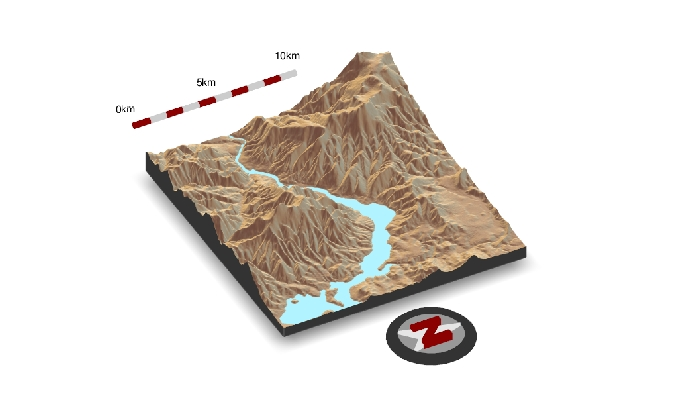
\includegraphics[width=1.2\textwidth,height=1.2\textheight]{J:/ENG 792/ENG_792-AVDR/ENG.792-AVDR/Cap_1_rayshader2.jpeg}

\hypertarget{como-r-funciona}{%
\section{Como R funciona}\label{como-r-funciona}}

Assista este conteúdo em \textbf{Cap 1 - Como R Funciona} no \href{https://www2.cead.ufv.br/sistemas/pvanet/geral/login.php}{PVANet}.

Diferentemente de outras linguagens, todos os comandos escritos são diretamente executados, desta forma o R não precisa de um compilador para executar os comandos como Fortran. Por isso, torna-se uma linguagem muito mais amigável e acessível para não programadores.

A linguagem é muito intuitiva (quase uma sintaxe lógica). Por exemplo uma regressão linear pode ser executada como \emph{lm(x\textasciitilde y)} ( \emph{\emph{lm}} vem de \emph{\emph{linear model}}). Como no exemplo do modelo linear acima, sempre que formos executar um comando temos que seguir da seguinte forma \emph{\emph{função(dados e demais ajustes ou parâmetros)}}, ou seja chame a função e coloque o resto dentro de parênteses.

Tudo que é executado pelo R fica armazenado na memória ativa (RAM) do computador na forma de objetos que possuem um nome. Os objetos, que variam em tipos e estruturas, podem ser funções criadas pelo próprio usuário, dados criados ou importados de uma memória, expressões e etc. Antes de entrarmos em detalhes sobre funções ou expressões, vamos nos ater aos objetos enquanto tipo e, na sequência, suas estruturas.

Dica de livro de cabeceira sobre R \citet{melloandpeternelli2013}.

Antes de avançarmos para os objetos é necessário fazer algumas recomendações e ressalvas.

Para criar um objeto qualquer podemos utilizar \textbf{\textless-} ou \textbf{=}. As boas práticas recomendam o uso de \textbf{\textless-} para evitar confusão já que o sinal \textbf{=} tem outras funções.

Um objeto é criado da seguinte forma \textbf{nome\_do\_objeto \textless- atribuição}.

\begin{Shaded}
\begin{Highlighting}[]
\NormalTok{nome\_do\_objeto }\OtherTok{\textless{}{-}} \StringTok{"atribuição"}
\NormalTok{nome\_do\_objeto}
\end{Highlighting}
\end{Shaded}

\begin{verbatim}
## [1] "atribuição"
\end{verbatim}

Contudo, evitem nomes longos, que comecem com numerais ou caracteres especiais ou letras maiúsculas (R é case-sensitive).
Caso sua linha de comando esteja ficando longa demais opte por quebrar a linha veremos isso mais adiante).

\hypertarget{tipos-de-objetos-mode-ou-type}{%
\subsection{\texorpdfstring{Tipos de objetos (\emph{mode} ou \emph{type})}{Tipos de objetos (mode ou type)}}\label{tipos-de-objetos-mode-ou-type}}

Os objetos no R podem ser do tipo \emph{lógico}, \emph{inteiro}, \emph{simples}, \emph{dupla}, \emph{complexo}, \emph{função} ou \emph{caractere}.

\begin{tabular}{l|l|l}
\hline
mode() & Armazenamento & Exemplo\\
\hline
logical & lógico & TRUE or FALSE\\
\hline
numeric & inteiro, simples ou dupla & Números 1, 3.14, 2e-308 etc\\
\hline
complex & complexo & 3+2i\\
\hline
function & função & Soma<-function(...)\\
\hline
name & caractere & média\\
\hline
\end{tabular}

\textbf{Tabela 1:} Tipos de modos para objetos no R.

\begin{Shaded}
\begin{Highlighting}[]
\CommentTok{\#logical}
\NormalTok{q1 }\OtherTok{\textless{}{-}}\NormalTok{T}
\FunctionTok{mode}\NormalTok{(q1);}\FunctionTok{typeof}\NormalTok{(q1)}
\end{Highlighting}
\end{Shaded}

\begin{verbatim}
## [1] "logical"
\end{verbatim}

\begin{verbatim}
## [1] "logical"
\end{verbatim}

\begin{Shaded}
\begin{Highlighting}[]
\NormalTok{q2 }\OtherTok{\textless{}{-}} \ConstantTok{FALSE} \CommentTok{\#pode ser a palavra toda mas em maiúsculas }
\FunctionTok{mode}\NormalTok{(q2);}\FunctionTok{typeof}\NormalTok{(q2)}
\end{Highlighting}
\end{Shaded}

\begin{verbatim}
## [1] "logical"
\end{verbatim}

\begin{verbatim}
## [1] "logical"
\end{verbatim}

\begin{Shaded}
\begin{Highlighting}[]
\CommentTok{\#integer}
\NormalTok{x}\OtherTok{\textless{}{-}}\NormalTok{2L }\CommentTok{\#L garante que 2 será integer}
\FunctionTok{mode}\NormalTok{(x);}\FunctionTok{typeof}\NormalTok{(x)}
\end{Highlighting}
\end{Shaded}

\begin{verbatim}
## [1] "numeric"
\end{verbatim}

\begin{verbatim}
## [1] "integer"
\end{verbatim}

\begin{Shaded}
\begin{Highlighting}[]
\CommentTok{\#double}
\NormalTok{y}\OtherTok{\textless{}{-}}\FloatTok{2.5}
\FunctionTok{mode}\NormalTok{(y);}\FunctionTok{typeof}\NormalTok{(y)}
\end{Highlighting}
\end{Shaded}

\begin{verbatim}
## [1] "numeric"
\end{verbatim}

\begin{verbatim}
## [1] "double"
\end{verbatim}

\begin{Shaded}
\begin{Highlighting}[]
\CommentTok{\#Complex}
\NormalTok{z}\OtherTok{\textless{}{-}}\DecValTok{3}\SpecialCharTok{+}\NormalTok{2i}
\FunctionTok{mode}\NormalTok{(z);}\FunctionTok{typeof}\NormalTok{(z)}
\end{Highlighting}
\end{Shaded}

\begin{verbatim}
## [1] "complex"
\end{verbatim}

\begin{verbatim}
## [1] "complex"
\end{verbatim}

\begin{Shaded}
\begin{Highlighting}[]
\CommentTok{\#function}
\NormalTok{Soma}\OtherTok{\textless{}{-}}\ControlFlowTok{function}\NormalTok{(x,y)\{}
\NormalTok{  x}\SpecialCharTok{+}\NormalTok{y}
\NormalTok{\}}
\FunctionTok{mode}\NormalTok{(Soma);}\FunctionTok{typeof}\NormalTok{(Soma)}
\end{Highlighting}
\end{Shaded}

\begin{verbatim}
## [1] "function"
\end{verbatim}

\begin{verbatim}
## [1] "closure"
\end{verbatim}

\begin{Shaded}
\begin{Highlighting}[]
\CommentTok{\#Character}
\NormalTok{a }\OtherTok{\textless{}{-}}\StringTok{"h"} \CommentTok{\#Para colocar uma letra em uma variável é preciso colocar entre "")}
\FunctionTok{mode}\NormalTok{(a);}\FunctionTok{typeof}\NormalTok{(a)}
\end{Highlighting}
\end{Shaded}

\begin{verbatim}
## [1] "character"
\end{verbatim}

\begin{verbatim}
## [1] "character"
\end{verbatim}

\begin{Shaded}
\begin{Highlighting}[]
\NormalTok{média}\OtherTok{\textless{}{-}}\StringTok{"média"}
\FunctionTok{mode}\NormalTok{(a);}\FunctionTok{typeof}\NormalTok{(a)}
\end{Highlighting}
\end{Shaded}

\begin{verbatim}
## [1] "character"
\end{verbatim}

\begin{verbatim}
## [1] "character"
\end{verbatim}

Saber as diferenças entre os diversos objetos é importante para uma exploração mais adequada dos dados, utilização eficiente de funções ou operações lógicas, artiméticas, estatísticas e etc.

Veja que no caso acima em \emph{integer} (x \textless- 2L) optamos por adicionar ``L'' após o número 2, pois o R por padrão decide onde e como aloca/aloja/armazena um operador. A informação será preferencialmente salva como \emph{double} e isso faz sentido caso você queira mais adiante realizar operações com números decimais ou realizar operações que resultem em números decimais.

No entanto, caso queira saber que tipo de dado está manipulando você pode ``perguntar'' utilizando \emph{is.} seguido da designação do tipo de dados quer testar ( \emph{integer}, \emph{numeric}, \emph{double} e etc) e teremos uma resposta lógica.

\begin{Shaded}
\begin{Highlighting}[]
\FunctionTok{is.double}\NormalTok{(x) }
\end{Highlighting}
\end{Shaded}

\begin{verbatim}
## [1] FALSE
\end{verbatim}

Caso você deseje que sua variável seja de um tipo específico, você pode transformá-la utilizando \emph{as.} seguido da designação desejada ( \emph{integer}, \emph{numeric}, \emph{double} e etc).

\begin{Shaded}
\begin{Highlighting}[]
\NormalTok{x}\OtherTok{\textless{}{-}}\FunctionTok{as.double}\NormalTok{(x)}
\FunctionTok{is.double}\NormalTok{(x)}
\end{Highlighting}
\end{Shaded}

\begin{verbatim}
## [1] TRUE
\end{verbatim}

Cada tipo de dado é associado com um teste e uma função de conversão conforme a tabela 2.

\begin{tabular}{l|l|l}
\hline
Tipo & Teste & Função de conversão\\
\hline
character & is.character & as.character\\
\hline
complex & is.complex & as.complex\\
\hline
double & is.double & as.double\\
\hline
expression & is.expression & as.expression\\
\hline
integer & is.integer & as.integer\\
\hline
list & is.list & as.list\\
\hline
logical & is.logical & as.logical\\
\hline
numeric & is.numeric & as.numeric\\
\hline
single & is.single & as.single\\
\hline
raw & is.raw & as.raw\\
\hline
Date & is.Date & as.Date\\
\hline
\end{tabular}

\textbf{Tabela 2:} Tipos de dados, teste e modos de conversão.

\hypertarget{estrutura-do-objetos-class}{%
\subsection{\texorpdfstring{Estrutura do objetos (\emph{class})}{Estrutura do objetos (class)}}\label{estrutura-do-objetos-class}}

As informações armazenadas em objetos no R podem ser organizadas em diferentes estruturas ou classes.

\begin{itemize}
\tightlist
\item
  No R existe uma grande variedade de classes de objetos, e sempre surgindo mais. No entanto, há classes de objetos que são mais comuns em situações em que estamos manipulando bases de dados, seja ela já existente, ou quando estamos criando com coleta usando técnicas de webscraping, por exemplo. São elas: interger, numeric, character, factor, matrix, data.frame e list. Uma coisa importante, no R não precisamos declarar qual classe vai ser o objeto unidimensional como em outras linguagem, embora possamos fazer isso, pois, o R aloca o objeto automaticamente em uma classe a partir do seu conteúdo. \citet{MeirelesandSilva2018}
\end{itemize}

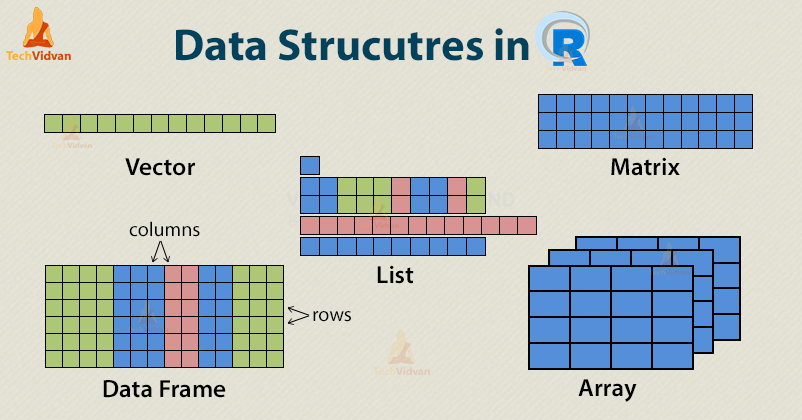
\includegraphics[width=0.5\textwidth,height=0.5\textheight]{J:/ENG 792/ENG_792-AVDR/ENG.792-AVDR/Cap_1_R_data_strucutres.jpg}

\textbf{Figura 1:} Estrutura de dados no R. Fonte: \href{https://techvidvan.com/tutorials/r-data-structures/}{techvidvan}

\begin{tabular}{l|l|l}
\hline
Objeto & modes & descrição\\
\hline
vector & numeric, character, complex ou logical & Com um ou  mais elementos\\
\hline
factor & numeric ou character & Vetor que representa dados categóricos\\
\hline
matriz & numeric, character, complex ou logical & Um array de duas dimensões\\
\hline
array & numeric, character, complex ou logical & Pode conter um, duas ou mais dimensões\\
\hline
data frame & numeric, character, complex ou logical & Um array de duas dimenões que permite colunas de diferentes tipos dem mesmo objeto\\
\hline
list & numeric, character, complex, logical, function, expression, ... & Objeto que permite combinar diferentes estruturtas de dados num único objeto\\
\hline
\end{tabular}

\textbf{Tabela 3:} Características dos tipos de objetos.

\hypertarget{vetores-vectors}{%
\subsubsection{\texorpdfstring{Vetores (\emph{Vectors})}{Vetores (Vectors)}}\label{vetores-vectors}}

Vetores são os tipos de objetos mais comuns no R. Um vetor é composto de uma informação ou uma séries de informações ( \emph{arrays} ) unidimensionais que podem conter informaçõs numéricas, caracteres ou dados lógicos.

Mesmo quando digitamos apenas um único elemento ele se torna um vetor de comprimento um (1).

\emph{Vetores com Apenas 1 elemento}

\begin{Shaded}
\begin{Highlighting}[]
\NormalTok{esquerdo}\OtherTok{\textless{}{-}}\NormalTok{(}\StringTok{"direito"}\NormalTok{) }\CommentTok{\# O objeto "esquerdo" recebe a palavra "direito"}
\NormalTok{esquerdo }\CommentTok{\#execute o arquivo e veja seu conteúdo}
\end{Highlighting}
\end{Shaded}

\begin{verbatim}
## [1] "direito"
\end{verbatim}

\begin{Shaded}
\begin{Highlighting}[]
\NormalTok{direito}\OtherTok{=}\FunctionTok{c}\NormalTok{(}\StringTok{"esquerdo"}\NormalTok{) }\CommentTok{\#Outra maneira de criar objeto  }
\FunctionTok{print}\NormalTok{(direito) }\CommentTok{\#Outra forma de executar o conteúdo}
\end{Highlighting}
\end{Shaded}

\begin{verbatim}
## [1] "esquerdo"
\end{verbatim}

\begin{Shaded}
\begin{Highlighting}[]
\NormalTok{b}\OtherTok{=}\NormalTok{(}\DecValTok{10}\NormalTok{) }\CommentTok{\# O objeto "b" recebe o número 10}
\NormalTok{b}
\end{Highlighting}
\end{Shaded}

\begin{verbatim}
## [1] 10
\end{verbatim}

\begin{Shaded}
\begin{Highlighting}[]
\NormalTok{(}\FloatTok{15.23}\NormalTok{)}\OtherTok{{-}\textgreater{}}\NormalTok{c }\CommentTok{\# O objeto "c" recebe o número 15.23}
\NormalTok{c}
\end{Highlighting}
\end{Shaded}

\begin{verbatim}
## [1] 15.23
\end{verbatim}

Vetores com múltiplos elementos.

\begin{Shaded}
\begin{Highlighting}[]
\NormalTok{d}\OtherTok{\textless{}{-}}\NormalTok{(}\DecValTok{0}\SpecialCharTok{:}\DecValTok{10}\NormalTok{) }\CommentTok{\# Criando uma sequência de 0 até 10}
\NormalTok{d}
\end{Highlighting}
\end{Shaded}

\begin{verbatim}
##  [1]  0  1  2  3  4  5  6  7  8  9 10
\end{verbatim}

\begin{Shaded}
\begin{Highlighting}[]
\NormalTok{e}\OtherTok{\textless{}{-}}\FloatTok{10.5}\SpecialCharTok{:}\FloatTok{20.5} \CommentTok{\# criando uma sequência de 10.5 até 20.5}
\NormalTok{e}
\end{Highlighting}
\end{Shaded}

\begin{verbatim}
##  [1] 10.5 11.5 12.5 13.5 14.5 15.5 16.5 17.5 18.5 19.5 20.5
\end{verbatim}

\begin{Shaded}
\begin{Highlighting}[]
\NormalTok{f}\OtherTok{\textless{}{-}}\NormalTok{(}\FloatTok{10.6}\SpecialCharTok{:}\FloatTok{20.3}\NormalTok{) }\CommentTok{\# O último elemento é descartado por nãos e encaixar na sequência}
\NormalTok{f}
\end{Highlighting}
\end{Shaded}

\begin{verbatim}
##  [1] 10.6 11.6 12.6 13.6 14.6 15.6 16.6 17.6 18.6 19.6
\end{verbatim}

Podemos utilizar também a função \emph{seq} para gerar uma sequêncaio de dados.

\emph{\emph{seq(from = 1, to = 1, by = ((to - from)/(length.out - 1)),length.out = NULL, along.with = NULL, \ldots)}}

\begin{Shaded}
\begin{Highlighting}[]
\NormalTok{g}\OtherTok{\textless{}{-}}\FunctionTok{seq}\NormalTok{(}\DecValTok{0}\NormalTok{,}\DecValTok{10}\NormalTok{,}\FloatTok{0.5}\NormalTok{) }\CommentTok{\# O objeto "g" recebe a sequência de 0 até 10 a cada 0.5}
\NormalTok{g}
\end{Highlighting}
\end{Shaded}

\begin{verbatim}
##  [1]  0.0  0.5  1.0  1.5  2.0  2.5  3.0  3.5  4.0  4.5  5.0  5.5  6.0  6.5  7.0
## [16]  7.5  8.0  8.5  9.0  9.5 10.0
\end{verbatim}

\begin{Shaded}
\begin{Highlighting}[]
\NormalTok{h}\OtherTok{\textless{}{-}}\FunctionTok{seq}\NormalTok{(}\AttributeTok{from=}\DecValTok{10}\NormalTok{,}\AttributeTok{to=}\DecValTok{20}\NormalTok{,}\AttributeTok{length.out=}\DecValTok{50}\NormalTok{) }\CommentTok{\# O objeto "h" recebe a sequência de 0 até 10 que é do compriumento 50, ou seja, há 50 número de 10 até 20}
\NormalTok{h}
\end{Highlighting}
\end{Shaded}

\begin{verbatim}
##  [1] 10.00000 10.20408 10.40816 10.61224 10.81633 11.02041 11.22449 11.42857
##  [9] 11.63265 11.83673 12.04082 12.24490 12.44898 12.65306 12.85714 13.06122
## [17] 13.26531 13.46939 13.67347 13.87755 14.08163 14.28571 14.48980 14.69388
## [25] 14.89796 15.10204 15.30612 15.51020 15.71429 15.91837 16.12245 16.32653
## [33] 16.53061 16.73469 16.93878 17.14286 17.34694 17.55102 17.75510 17.95918
## [41] 18.16327 18.36735 18.57143 18.77551 18.97959 19.18367 19.38776 19.59184
## [49] 19.79592 20.00000
\end{verbatim}

Experimente também a função \emph{rep()}.

\emph{\emph{rep(x, times = 1, length.out = NA, each = 1)}}

\begin{Shaded}
\begin{Highlighting}[]
\NormalTok{i}\OtherTok{\textless{}{-}}\FunctionTok{rep}\NormalTok{(}\DecValTok{0}\NormalTok{,}\DecValTok{10}\NormalTok{) }\CommentTok{\# O objeto "i" recebe 10 números 1}
\NormalTok{i}
\end{Highlighting}
\end{Shaded}

\begin{verbatim}
##  [1] 0 0 0 0 0 0 0 0 0 0
\end{verbatim}

\begin{Shaded}
\begin{Highlighting}[]
\NormalTok{j}\OtherTok{\textless{}{-}}\FunctionTok{rep}\NormalTok{(}\FunctionTok{c}\NormalTok{(}\DecValTok{1}\SpecialCharTok{:}\DecValTok{3}\NormalTok{),}\DecValTok{10}\NormalTok{) }\CommentTok{\# O objeto "j" recebe 10 vezes a sequência 1, 2 e 3}
\NormalTok{j}
\end{Highlighting}
\end{Shaded}

\begin{verbatim}
##  [1] 1 2 3 1 2 3 1 2 3 1 2 3 1 2 3 1 2 3 1 2 3 1 2 3 1 2 3 1 2 3
\end{verbatim}

\textbf{Um Vetor só pode conter informações de um único tipo!}

\begin{Shaded}
\begin{Highlighting}[]
\NormalTok{k}\OtherTok{\textless{}{-}}\FunctionTok{c}\NormalTok{(}\DecValTok{0}\NormalTok{,}\DecValTok{1}\NormalTok{,}\DecValTok{2}\NormalTok{,}\DecValTok{3}\NormalTok{,}\DecValTok{4}\NormalTok{, }\StringTok{"A"}\NormalTok{) }\CommentTok{\# O objeto "k" é do tipo character por causa de "A"}
\FunctionTok{typeof}\NormalTok{(k);}\FunctionTok{mode}\NormalTok{(k)}
\end{Highlighting}
\end{Shaded}

\begin{verbatim}
## [1] "character"
\end{verbatim}

\begin{verbatim}
## [1] "character"
\end{verbatim}

\begin{Shaded}
\begin{Highlighting}[]
\NormalTok{l}\OtherTok{\textless{}{-}}\FunctionTok{c}\NormalTok{(}\DecValTok{0}\NormalTok{,}\DecValTok{1}\NormalTok{,}\DecValTok{2}\NormalTok{,}\DecValTok{3}\NormalTok{,}\DecValTok{4}\NormalTok{) }\CommentTok{\# O objeto "l" é do tipo numérico}
\FunctionTok{typeof}\NormalTok{(l);}\FunctionTok{mode}\NormalTok{(l)}
\end{Highlighting}
\end{Shaded}

\begin{verbatim}
## [1] "double"
\end{verbatim}

\begin{verbatim}
## [1] "numeric"
\end{verbatim}

\hypertarget{fatores-factors}{%
\subsubsection{\texorpdfstring{Fatores (\emph{Factors})}{Fatores (Factors)}}\label{fatores-factors}}

Os fatores são vetores em que os elementos pertencem a uma ou mais categorias temáticas.
As variáveis aleatórias podem ser divididas em contínuas e categóricas.

\begin{itemize}
\tightlist
\item
  As contínuas podem ser medidas nas escalas: relacional e intervalar.
\item
  As categóricas nas escalas: nominal e ordinal.
\end{itemize}

No R, as variáveis categóricas medidas nas escalas nominal e ordinal são chamados fatores.
A função \emph{factor()} armazena os valores categóricos como um vetor de inteiros {[}1..k{]} e um vetor interno de \emph{strings} referentes ao nomes.
\emph{Em outras palavras, um \textbf{factor} é um \textbf{vetor} objeto usado para especificar uma classsificação discreta (agrupamento) dos componentes de outros vetores de mesmo tamanho.}

\emph{\emph{factor(x = character(), levels, labels = levels,exclude = NA, ordered = is.ordered(x), nmax = NA)}}

ou

\emph{\emph{gl(n, k, length = n X k, labels = seq\_len(n), ordered = FALSE)}}

\begin{Shaded}
\begin{Highlighting}[]
\NormalTok{m}\OtherTok{\textless{}{-}}\FunctionTok{factor}\NormalTok{(}\FunctionTok{c}\NormalTok{(}\StringTok{"H"}\NormalTok{,}\StringTok{"H"}\NormalTok{,}\StringTok{"H"}\NormalTok{,}\StringTok{"M"}\NormalTok{,}\StringTok{"M"}\NormalTok{)) }\CommentTok{\# O objeto "k" recebe 3 H\textquotesingle{}s e 2 M\textquotesingle{}s}
\NormalTok{m}
\end{Highlighting}
\end{Shaded}

\begin{verbatim}
## [1] H H H M M
## Levels: H M
\end{verbatim}

\begin{Shaded}
\begin{Highlighting}[]
\FunctionTok{as.integer}\NormalTok{(m)}
\end{Highlighting}
\end{Shaded}

\begin{verbatim}
## [1] 1 1 1 2 2
\end{verbatim}

\begin{Shaded}
\begin{Highlighting}[]
\NormalTok{n}\OtherTok{\textless{}{-}}\FunctionTok{gl}\NormalTok{(}\AttributeTok{n=}\DecValTok{2}\NormalTok{,}\AttributeTok{k=}\DecValTok{3}\NormalTok{,}\AttributeTok{labels=}\FunctionTok{c}\NormalTok{(}\StringTok{"M"}\NormalTok{,}\StringTok{"F"}\NormalTok{)) }
\NormalTok{n}
\end{Highlighting}
\end{Shaded}

\begin{verbatim}
## [1] M M M F F F
## Levels: M F
\end{verbatim}

Podemos verificar os níveis de um fator usando o comando \emph{levels()}.

\begin{Shaded}
\begin{Highlighting}[]
\FunctionTok{levels}\NormalTok{(m)}
\end{Highlighting}
\end{Shaded}

\begin{verbatim}
## [1] "H" "M"
\end{verbatim}

\begin{Shaded}
\begin{Highlighting}[]
\FunctionTok{levels}\NormalTok{(n)}
\end{Highlighting}
\end{Shaded}

\begin{verbatim}
## [1] "M" "F"
\end{verbatim}

\hypertarget{matriz-matrix}{%
\subsubsection{\texorpdfstring{Matriz (\emph{Matrix})}{Matriz (Matrix)}}\label{matriz-matrix}}

É o tipo de dado mais comum que encontramos do dia a dia. A maioria dos dados que analisamos estão organizados em matrizes que são dados combinados em 2 dimensões (linhas e colunas).
Existem várias maneiras de criar uma matriz como utilizando o comando \emph{matrix()}.

\emph{\emph{matrix(data = NA, nrow = 1, ncol = 1, byrow = FALSE,dimnames = NULL)}}

Assim como os vetores, as matrizes só aceitam dados do mesmo tipo.

\begin{Shaded}
\begin{Highlighting}[]
\NormalTok{o}\OtherTok{\textless{}{-}}\DecValTok{1}\SpecialCharTok{:}\DecValTok{10} \CommentTok{\# cria um vetor de 1 a 10}
\NormalTok{o\_matriz1}\OtherTok{\textless{}{-}}\FunctionTok{matrix}\NormalTok{(o,}\AttributeTok{ncol=}\DecValTok{5}\NormalTok{)}\CommentTok{\# Organiza o vetor "o" e 5 colunas}
\NormalTok{o\_matriz1}
\end{Highlighting}
\end{Shaded}

\begin{verbatim}
##      [,1] [,2] [,3] [,4] [,5]
## [1,]    1    3    5    7    9
## [2,]    2    4    6    8   10
\end{verbatim}

\begin{Shaded}
\begin{Highlighting}[]
\NormalTok{o\_matriz2}\OtherTok{\textless{}{-}}\FunctionTok{matrix}\NormalTok{(o,}\AttributeTok{nrow=}\DecValTok{5}\NormalTok{)}\CommentTok{\# Organiza o vetor "o" e 5 linhas}
\NormalTok{o\_matriz2}
\end{Highlighting}
\end{Shaded}

\begin{verbatim}
##      [,1] [,2]
## [1,]    1    6
## [2,]    2    7
## [3,]    3    8
## [4,]    4    9
## [5,]    5   10
\end{verbatim}

Podemos utilizar também o argumento \emph{byrow=}, que, diferente do exemplo acima, preenche a tabela por linha.

\begin{Shaded}
\begin{Highlighting}[]
\NormalTok{p}\OtherTok{\textless{}{-}}\DecValTok{1}\SpecialCharTok{:}\DecValTok{10} \CommentTok{\# cria um vetor de 1 a 10}
\NormalTok{p\_matriz1}\OtherTok{\textless{}{-}}\FunctionTok{matrix}\NormalTok{(o,}\AttributeTok{nrow=}\DecValTok{5}\NormalTok{,}\AttributeTok{byrow=}\NormalTok{T)}\CommentTok{\# Organiza o vetor "o" e 5 colunas}
\NormalTok{p\_matriz1; o\_matriz2 }\CommentTok{\# compare os 2 modos}
\end{Highlighting}
\end{Shaded}

\begin{verbatim}
##      [,1] [,2]
## [1,]    1    2
## [2,]    3    4
## [3,]    5    6
## [4,]    7    8
## [5,]    9   10
\end{verbatim}

\begin{verbatim}
##      [,1] [,2]
## [1,]    1    6
## [2,]    2    7
## [3,]    3    8
## [4,]    4    9
## [5,]    5   10
\end{verbatim}

As dimensões de uma matriz podem ser acessadas através do comando \emph{dim()}:

\begin{Shaded}
\begin{Highlighting}[]
\FunctionTok{dim}\NormalTok{(o\_matriz1);}\FunctionTok{dim}\NormalTok{(o\_matriz2) }\CommentTok{\# Leia o o resultado como linha e coluna}
\end{Highlighting}
\end{Shaded}

\begin{verbatim}
## [1] 2 5
\end{verbatim}

\begin{verbatim}
## [1] 5 2
\end{verbatim}

Também é interessante usar o comando \emph{summary()}.

\begin{Shaded}
\begin{Highlighting}[]
\FunctionTok{summary}\NormalTok{(o\_matriz1);}\FunctionTok{summary}\NormalTok{(o\_matriz2) }\CommentTok{\# Mostra informações por coluna}
\end{Highlighting}
\end{Shaded}

\begin{verbatim}
##        V1             V2             V3             V4             V5       
##  Min.   :1.00   Min.   :3.00   Min.   :5.00   Min.   :7.00   Min.   : 9.00  
##  1st Qu.:1.25   1st Qu.:3.25   1st Qu.:5.25   1st Qu.:7.25   1st Qu.: 9.25  
##  Median :1.50   Median :3.50   Median :5.50   Median :7.50   Median : 9.50  
##  Mean   :1.50   Mean   :3.50   Mean   :5.50   Mean   :7.50   Mean   : 9.50  
##  3rd Qu.:1.75   3rd Qu.:3.75   3rd Qu.:5.75   3rd Qu.:7.75   3rd Qu.: 9.75  
##  Max.   :2.00   Max.   :4.00   Max.   :6.00   Max.   :8.00   Max.   :10.00
\end{verbatim}

\begin{verbatim}
##        V1          V2    
##  Min.   :1   Min.   : 6  
##  1st Qu.:2   1st Qu.: 7  
##  Median :3   Median : 8  
##  Mean   :3   Mean   : 8  
##  3rd Qu.:4   3rd Qu.: 9  
##  Max.   :5   Max.   :10
\end{verbatim}

Outras formas de construir matrizes é juntando objetos existentes através dos comandos \emph{cbind()} e \emph{rbind()} que concatenam objetos por colunas e linhas, respectivamente.

Vamos juntar as matrizes já criadas.

\begin{Shaded}
\begin{Highlighting}[]
\NormalTok{o\_matriz3}\OtherTok{\textless{}{-}}\FunctionTok{rbind}\NormalTok{(o\_matriz1,o\_matriz1) }\CommentTok{\# concatena por linhas (row)}
\NormalTok{o\_matriz3}
\end{Highlighting}
\end{Shaded}

\begin{verbatim}
##      [,1] [,2] [,3] [,4] [,5]
## [1,]    1    3    5    7    9
## [2,]    2    4    6    8   10
## [3,]    1    3    5    7    9
## [4,]    2    4    6    8   10
\end{verbatim}

\begin{Shaded}
\begin{Highlighting}[]
\NormalTok{o\_matriz4}\OtherTok{\textless{}{-}}\FunctionTok{cbind}\NormalTok{(o\_matriz2,o\_matriz2) }\CommentTok{\# concatena por colunas (column)}
\NormalTok{o\_matriz4}
\end{Highlighting}
\end{Shaded}

\begin{verbatim}
##      [,1] [,2] [,3] [,4]
## [1,]    1    6    1    6
## [2,]    2    7    2    7
## [3,]    3    8    3    8
## [4,]    4    9    4    9
## [5,]    5   10    5   10
\end{verbatim}

\hypertarget{array}{%
\subsubsection{Array}\label{array}}

O array é um conjunto de matrizes ou vetores que podem ter qualquer número de dimensões. Estas dimensões podem receber nomes.
Podemos criar \emph{arrays} atribuindo dimensções a um vetor com o comando \emph{dim()} ou usando \emph{array()}.

\emph{\emph{array(data = NA, dim = length(data), dimnames = NULL)}}

\begin{Shaded}
\begin{Highlighting}[]
\NormalTok{q\_array}\OtherTok{\textless{}{-}}\DecValTok{1}\SpecialCharTok{:}\DecValTok{12} \CommentTok{\# cria um vetor}
\FunctionTok{dim}\NormalTok{(q\_array)}\OtherTok{\textless{}{-}}\FunctionTok{c}\NormalTok{(}\DecValTok{2}\NormalTok{,}\DecValTok{3}\NormalTok{,}\DecValTok{2}\NormalTok{) }\CommentTok{\# atribuindo 3 dimensões a q\_array}
\NormalTok{q\_array}
\end{Highlighting}
\end{Shaded}

\begin{verbatim}
## , , 1
## 
##      [,1] [,2] [,3]
## [1,]    1    3    5
## [2,]    2    4    6
## 
## , , 2
## 
##      [,1] [,2] [,3]
## [1,]    7    9   11
## [2,]    8   10   12
\end{verbatim}

\begin{Shaded}
\begin{Highlighting}[]
\NormalTok{r\_array}\OtherTok{\textless{}{-}}\FunctionTok{array}\NormalTok{(}\DecValTok{1}\SpecialCharTok{:}\DecValTok{12}\NormalTok{,}\FunctionTok{c}\NormalTok{(}\DecValTok{2}\NormalTok{,}\DecValTok{3}\NormalTok{,}\DecValTok{2}\NormalTok{)) }\CommentTok{\# cria um array de 3 dimensões}
\NormalTok{r\_array}
\end{Highlighting}
\end{Shaded}

\begin{verbatim}
## , , 1
## 
##      [,1] [,2] [,3]
## [1,]    1    3    5
## [2,]    2    4    6
## 
## , , 2
## 
##      [,1] [,2] [,3]
## [1,]    7    9   11
## [2,]    8   10   12
\end{verbatim}

\hypertarget{data-frame}{%
\subsubsection{Data Frame}\label{data-frame}}

Tão comum quanto a matriz, o data frame também um modo bidimensional de organização dos dados (linhas e colunas) que, diferentemente da matriz, permite objetos de tipos diferentes (character, numeric, logical e etc) sejam armazenados.
Normalmente, nos data frames temos nas linhas as observações e nas colunas temos as variáveis.
No entanto, é importante que cada coluna tenha o mesmo tamanho.

\emph{\emph{data.frame(\ldots, row.names = NULL, check.rows = FALSE,check.names = TRUE, fix.empty.names = TRUE,stringsAsFactors = default.stringsAsFactors())}}

\begin{table}
\centering\begingroup\fontsize{11.5}{13.5}\selectfont

\begin{tabular}{l|l|l|l|l|l|l|l|l|l|l}
\hline
Equipes & Jogos & Vitórias & Empates & Derrotas & Gols Pró & Gols Contra & Pontos & Saldo de Gols & Aprov  & Destino\\
\hline
Flamengo & 38 & 28 & 6 & 4 & 86 & 37 & 90 & 49 & 79 & Libertadores\\
\hline
Santos & 38 & 22 & 8 & 8 & 60 & 33 & 74 & 27 & 65 & Libertadores\\
\hline
Palmeiras & 38 & 21 & 11 & 6 & 61 & 32 & 74 & 29 & 65 & Libertadores\\
\hline
Grêmio & 38 & 19 & 8 & 11 & 64 & 39 & 65 & 25 & 57 & Libertadores\\
\hline
Athletico Paranaense & 38 & 18 & 10 & 10 & 51 & 32 & 64 & 19 & 56 & Libertadores\\
\hline
Sao Paulo & 38 & 17 & 12 & 9 & 39 & 30 & 63 & 9 & 55 & Libertadores\\
\hline
Internacional & 38 & 16 & 9 & 13 & 44 & 39 & 57 & 5 & 5 & Libertadores\\
\hline
Corinthians & 38 & 14 & 14 & 10 & 42 & 34 & 56 & 8 & 49 & Libertadores\\
\hline
Fortaleza & 38 & 15 & 8 & 15 & 50 & 49 & 53 & 1 & 46 & Sulamericana\\
\hline
Goiás & 38 & 15 & 7 & 16 & 46 & 64 & 52 & -18 & 46 & Sulamericana\\
\hline
Bahia & 38 & 12 & 13 & 13 & 44 & 43 & 49 & 1 & 43 & Sulamericana\\
\hline
Vasco da Gama & 38 & 12 & 13 & 13 & 39 & 45 & 49 & -6 & 43 & Sulamericana\\
\hline
Atlético Mineiro & 38 & 13 & 9 & 16 & 45 & 49 & 48 & -4 & 42 & Sulamericana\\
\hline
Fluminense & 38 & 12 & 10 & 16 & 38 & 46 & 46 & -8 & 4 & Sulamericana\\
\hline
Botafogo & 38 & 13 & 4 & 21 & 31 & 45 & 43 & -14 & 38 & NA\\
\hline
Ceará & 38 & 10 & 9 & 19 & 36 & 41 & 39 & -5 & 34 & NA\\
\hline
Cruzeiro & 38 & 7 & 15 & 16 & 27 & 46 & 36 & -19 & 32 & Rebaixado\\
\hline
CSA & 38 & 8 & 8 & 22 & 24 & 58 & 32 & -34 & 28 & Rebaixado\\
\hline
Chapecoense & 38 & 7 & 11 & 20 & 31 & 52 & 32 & -21 & 28 & Rebaixado\\
\hline
Avaí & 38 & 3 & 11 & 24 & 18 & 62 & 20 & -44 & 18 & Rebaixado\\
\hline
\end{tabular}
\endgroup{}
\end{table}

\textbf{Tabela 3:} Data frame do resultados final do Campeonato Brasileiro de 2019.

\begin{Shaded}
\begin{Highlighting}[]
\NormalTok{Nome}\OtherTok{\textless{}{-}}\FunctionTok{c}\NormalTok{(}\StringTok{"A"}\NormalTok{, }\StringTok{"B"}\NormalTok{, }\StringTok{"C"}\NormalTok{)}
\NormalTok{Idade}\OtherTok{\textless{}{-}}\FunctionTok{c}\NormalTok{(}\DecValTok{25}\NormalTok{, }\DecValTok{32}\NormalTok{, }\DecValTok{28}\NormalTok{)}
\NormalTok{Sexo}\OtherTok{\textless{}{-}}\FunctionTok{c}\NormalTok{(}\StringTok{"M"}\NormalTok{,}\StringTok{"M"}\NormalTok{, }\StringTok{"F"}\NormalTok{)}
\NormalTok{Nome;Idade;Sexo}
\end{Highlighting}
\end{Shaded}

\begin{verbatim}
## [1] "A" "B" "C"
\end{verbatim}

\begin{verbatim}
## [1] 25 32 28
\end{verbatim}

\begin{verbatim}
## [1] "M" "M" "F"
\end{verbatim}

\begin{Shaded}
\begin{Highlighting}[]
\NormalTok{Ficha}\OtherTok{\textless{}{-}}\FunctionTok{data.frame}\NormalTok{(Nome,Idade,Sexo)}

\FunctionTok{attributes}\NormalTok{(Ficha) }\CommentTok{\# exibe os atributos do data frame}
\end{Highlighting}
\end{Shaded}

\begin{verbatim}
## $names
## [1] "Nome"  "Idade" "Sexo" 
## 
## $class
## [1] "data.frame"
## 
## $row.names
## [1] 1 2 3
\end{verbatim}

\begin{tabular}{l|c|c}
\hline
Nome & Idade & Sexo\\
\hline
A & 25 & M\\
\hline
B & 32 & M\\
\hline
C & 28 & F\\
\hline
\end{tabular}

\textbf{Tabela 4:} Tabela com dados fictícios.

\hypertarget{lista-list}{%
\subsubsection{\texorpdfstring{Lista (\emph{list})}{Lista (list)}}\label{lista-list}}

\emph{List} permite combinar diferentes estruturas de dados em um mesmo objeto, ou seja, \emph{vetores}, \emph{matrizes}, \emph{arrays}, \emph{data.frames} e até outras listas.
As listas são construídas utilizando o comando \emph{list()}.

Os componentes da lista são criados da mesma maneira como para \emph{data.frame}.
\textbf{list(\ldots)}

\begin{Shaded}
\begin{Highlighting}[]
\NormalTok{Nome}\OtherTok{\textless{}{-}}\FunctionTok{c}\NormalTok{(}\StringTok{"A"}\NormalTok{)}
\NormalTok{Idade}\OtherTok{\textless{}{-}}\FunctionTok{c}\NormalTok{(}\DecValTok{25}\NormalTok{)}
\NormalTok{Sexo}\OtherTok{\textless{}{-}}\FunctionTok{c}\NormalTok{(}\StringTok{"M"}\NormalTok{)}
\NormalTok{Notas}\OtherTok{\textless{}{-}}\FunctionTok{c}\NormalTok{(}\DecValTok{55}\NormalTok{,}\DecValTok{42}\NormalTok{,}\DecValTok{50}\NormalTok{,}\DecValTok{35}\NormalTok{)}
\NormalTok{Nome;Idade;Sexo;Notas}
\end{Highlighting}
\end{Shaded}

\begin{verbatim}
## [1] "A"
\end{verbatim}

\begin{verbatim}
## [1] 25
\end{verbatim}

\begin{verbatim}
## [1] "M"
\end{verbatim}

\begin{verbatim}
## [1] 55 42 50 35
\end{verbatim}

\begin{Shaded}
\begin{Highlighting}[]
\NormalTok{Desempenho}\OtherTok{\textless{}{-}}\FunctionTok{list}\NormalTok{(}\AttributeTok{nome=}\StringTok{"A"}\NormalTok{, }\AttributeTok{idade=}\DecValTok{25}\NormalTok{, }\AttributeTok{Sexo=}\StringTok{"M"}\NormalTok{,}\AttributeTok{Notas=}\FunctionTok{c}\NormalTok{(}\DecValTok{55}\NormalTok{,}\DecValTok{42}\NormalTok{,}\DecValTok{50}\NormalTok{,}\DecValTok{35}\NormalTok{))}
\NormalTok{Desempenho}
\end{Highlighting}
\end{Shaded}

\begin{verbatim}
## $nome
## [1] "A"
## 
## $idade
## [1] 25
## 
## $Sexo
## [1] "M"
## 
## $Notas
## [1] 55 42 50 35
\end{verbatim}

\begin{Shaded}
\begin{Highlighting}[]
\FunctionTok{is.list}\NormalTok{(Desempenho)}
\end{Highlighting}
\end{Shaded}

\begin{verbatim}
## [1] TRUE
\end{verbatim}

Existem também alguns comandos/funções que mostram resultados como listas.

\begin{Shaded}
\begin{Highlighting}[]
\NormalTok{s}\OtherTok{\textless{}{-}}\FunctionTok{c}\NormalTok{(}\DecValTok{1}\SpecialCharTok{:}\DecValTok{30}\NormalTok{)}
\NormalTok{t}\OtherTok{\textless{}{-}}\FunctionTok{c}\NormalTok{(}\DecValTok{30}\SpecialCharTok{:}\DecValTok{59}\NormalTok{)}

\NormalTok{teste.t}\OtherTok{\textless{}{-}}\FunctionTok{t.test}\NormalTok{(s,t, }\AttributeTok{var.equal =}\NormalTok{ T) }\CommentTok{\# calcula o test t para 2 amostras de variâncias iguais}
\NormalTok{teste.t}
\end{Highlighting}
\end{Shaded}

\begin{verbatim}
## 
##  Two Sample t-test
## 
## data:  s and t
## t = -12.758, df = 58, p-value < 2.2e-16
## alternative hypothesis: true difference in means is not equal to 0
## 95 percent confidence interval:
##  -33.54996 -24.45004
## sample estimates:
## mean of x mean of y 
##      15.5      44.5
\end{verbatim}

\begin{Shaded}
\begin{Highlighting}[]
\FunctionTok{is.list}\NormalTok{(teste.t);}\FunctionTok{mode}\NormalTok{(teste.t)}
\end{Highlighting}
\end{Shaded}

\begin{verbatim}
## [1] TRUE
\end{verbatim}

\begin{verbatim}
## [1] "list"
\end{verbatim}

Para finalizar por hoje preste atenção no seu \emph{Global Environment}.
Veja que há uma grande quantidade de objetos lá. Agora execute o comando abaixo:

\begin{Shaded}
\begin{Highlighting}[]
\FunctionTok{rm}\NormalTok{(Desempenho)}

\FunctionTok{rm}\NormalTok{(}\AttributeTok{list=}\FunctionTok{ls}\NormalTok{())}
\end{Highlighting}
\end{Shaded}

Voilà! Sumiu tudo.

\hypertarget{acessando-e-manipulauxe7uxe3o-de-dados}{%
\chapter{Acessando e manipulação de dados}\label{acessando-e-manipulauxe7uxe3o-de-dados}}

\hypertarget{organizauxe7uxe3o}{%
\section{Organização}\label{organizauxe7uxe3o}}

Como mencionado anteriormente, \texttt{vector} é uma das principais estruturas do \textbf{R}. Um vetor é uma sequência de elementos (1\ldots n) do mesmo tipo organizados tal qual livros em uma prateleira.\\
No caso abaixo temos um vetor numérico que pode ser \texttt{integer} ou \texttt{double}.

\begin{Shaded}
\begin{Highlighting}[]
\NormalTok{a}\OtherTok{\textless{}{-}}\FunctionTok{c}\NormalTok{(}\DecValTok{25}\NormalTok{,}\DecValTok{17}\NormalTok{,}\DecValTok{55}\NormalTok{,}\DecValTok{3}\NormalTok{,}\DecValTok{12}\NormalTok{,}\DecValTok{315}\NormalTok{,}\DecValTok{10}\NormalTok{,}\DecValTok{2}\NormalTok{,}\DecValTok{3}\NormalTok{,}\DecValTok{11}\NormalTok{)}
\NormalTok{a}
\end{Highlighting}
\end{Shaded}

\begin{verbatim}
##  [1]  25  17  55   3  12 315  10   2   3  11
\end{verbatim}

\begin{longtable}[]{@{}ccccccccccc@{}}
\toprule
Posição & 1 & 2 & 3 & 4 & 5 & 6 & 7 & 8 & 9 & 10 \\
\midrule
\endhead
Elementos & 25 & 17 & 55 & 3 & 12 & 315 & 10 & 2 & 3 & 11 \\
\bottomrule
\end{longtable}

Um vetor também pode armazernar caracteres. Neste caso eles devem estar entre aspas duplas \texttt{("")}.

\begin{Shaded}
\begin{Highlighting}[]
\NormalTok{b}\OtherTok{\textless{}{-}}\FunctionTok{c}\NormalTok{(}\StringTok{"Z"}\NormalTok{,}\StringTok{"f"}\NormalTok{, }\StringTok{"7"}\NormalTok{,}\StringTok{"2a"}\NormalTok{,}\StringTok{"Yes"}\NormalTok{,}\StringTok{"A"}\NormalTok{,}\StringTok{"Ab"}\NormalTok{)}
\NormalTok{b;}\FunctionTok{typeof}\NormalTok{(b)}
\end{Highlighting}
\end{Shaded}

\begin{verbatim}
## [1] "Z"   "f"   "7"   "2a"  "Yes" "A"   "Ab"
\end{verbatim}

\begin{verbatim}
## [1] "character"
\end{verbatim}

Embora tenhamos o número \emph{7} entre os nossos elementos do vetor acima, por estar entre aspas o número \emph{7} não é \texttt{numéric}, mas caractere.\\
Lembrem-se que um \texttt{vector} é um banco de dados da mesmo tipo Logo, se você colocar um número \emph{7} dentro dele, o \textbf{R} vai automaticamente convertê-lo em caractere independente de estar entre \texttt{""} ou não.

\begin{longtable}[]{@{}cccccccc@{}}
\toprule
Posição & 1 & 2 & 3 & 4 & 5 & 6 & 7 \\
\midrule
\endhead
Elementos & ``Z'' & ``f'' & ``7'' & ``2a'' & ``Yes'' & ``A'' & ``Ab'' \\
\bottomrule
\end{longtable}

Mesmo que você tenha apenas um único numeral ele será armazenado como vector, vector de \textbf{comprimento = 1}.
Então um único número ou um único caractere será um vector.

\begin{Shaded}
\begin{Highlighting}[]
\NormalTok{c}\OtherTok{\textless{}{-}}\NormalTok{(}\DecValTok{1}\NormalTok{)}
\NormalTok{c;}\FunctionTok{typeof}\NormalTok{(c);}\FunctionTok{is.vector}\NormalTok{(c)}
\end{Highlighting}
\end{Shaded}

\begin{verbatim}
## [1] 1
\end{verbatim}

\begin{verbatim}
## [1] "double"
\end{verbatim}

\begin{verbatim}
## [1] TRUE
\end{verbatim}

\begin{longtable}[]{@{}cc@{}}
\toprule
Posição & 1 \\
\midrule
\endhead
Elemento & ``1'' \\
\bottomrule
\end{longtable}

Entender a posição de cada elemento dentro de um \texttt{vector} é crucial! Saber a posição correta onde determinado(s) elemento(s) está(estão) facilita em muito nossa limpeza, nosso tratamento e demais passos para uma eficiente manipulação dos dados.

\begin{Shaded}
\begin{Highlighting}[]
\FunctionTok{seq}\NormalTok{(}\DecValTok{100}\NormalTok{,}\DecValTok{50}\NormalTok{,}\SpecialCharTok{{-}}\DecValTok{1}\NormalTok{)}
\end{Highlighting}
\end{Shaded}

\begin{verbatim}
##  [1] 100  99  98  97  96  95  94  93  92  91  90  89  88  87  86  85  84  83  82
## [20]  81  80  79  78  77  76  75  74  73  72  71  70  69  68  67  66  65  64  63
## [39]  62  61  60  59  58  57  56  55  54  53  52  51  50
\end{verbatim}

Atenção para os números dentro dos colchetes \texttt{{[}1{]}\ {[}17{]}\ {[}33{]}\ {[}49{]}}. Como mencionado em aulas passadas, eles, os colchetes, indicam a posição de determinados elementos dentro de um banco de dados.\\
Especificamente o \texttt{{[}1{]}} informa que o número \emph{100} é o primeiro elemento, \texttt{{[}17{]}} informa que o número \emph{84} é o vigésimo elemento, \texttt{{[}33{]}} informa que o número \emph{68} é o trigésimo nono elemento, \texttt{{[}49{]}} informa que o número \emph{52} é o trigésimo nono elemento.

\hypertarget{usando---subscribing-ou-indexing}{%
\subsection{Usando {[} {]} - Subscribing ou indexing}\label{usando---subscribing-ou-indexing}}

\hypertarget{vetores}{%
\subsubsection{Vetores}\label{vetores}}

Podemos extrapolar esta ideia de utilização de \texttt{{[}{]}} para acessar informações dentros dos objetos que criamos ou importamos.

\begin{Shaded}
\begin{Highlighting}[]
\NormalTok{d}\OtherTok{\textless{}{-}}\FunctionTok{c}\NormalTok{(}\StringTok{"a"}\NormalTok{,}\StringTok{"b"}\NormalTok{,}\StringTok{"c"}\NormalTok{,}\StringTok{"d"}\NormalTok{,}\StringTok{"e"}\NormalTok{)}
\NormalTok{d}
\end{Highlighting}
\end{Shaded}

\begin{verbatim}
## [1] "a" "b" "c" "d" "e"
\end{verbatim}

\begin{longtable}[]{@{}cccccc@{}}
\toprule
Posição & 1 & 2 & 3 & 4 & 5 \\
\midrule
\endhead
Elementos & ``a'' & ``b'' & ``c'' & ``d'' & ``e'' \\
\bottomrule
\end{longtable}

No \texttt{vector\ d} temos cada um dos elementos em sua respectiva posição. Para acessar um elemento específico podemos inserir o número refere à sua posição dentro de \texttt{{[}{]}}.\\
Por exemplo:

\begin{Shaded}
\begin{Highlighting}[]
\NormalTok{d[}\DecValTok{1}\NormalTok{]}
\end{Highlighting}
\end{Shaded}

\begin{verbatim}
## [1] "a"
\end{verbatim}

\begin{Shaded}
\begin{Highlighting}[]
\NormalTok{d[}\DecValTok{2}\NormalTok{]}
\end{Highlighting}
\end{Shaded}

\begin{verbatim}
## [1] "b"
\end{verbatim}

\begin{Shaded}
\begin{Highlighting}[]
\NormalTok{d[}\DecValTok{3}\NormalTok{]}
\end{Highlighting}
\end{Shaded}

\begin{verbatim}
## [1] "c"
\end{verbatim}

\begin{Shaded}
\begin{Highlighting}[]
\NormalTok{d[}\DecValTok{4}\NormalTok{]}
\end{Highlighting}
\end{Shaded}

\begin{verbatim}
## [1] "d"
\end{verbatim}

\begin{Shaded}
\begin{Highlighting}[]
\NormalTok{d[}\DecValTok{5}\NormalTok{]}
\end{Highlighting}
\end{Shaded}

\begin{verbatim}
## [1] "e"
\end{verbatim}

Importante saber que \texttt{{[}{]}} é muito versátil.

\begin{Shaded}
\begin{Highlighting}[]
\NormalTok{d[}\SpecialCharTok{{-}}\DecValTok{1}\NormalTok{] }\CommentTok{\# Acessa todos elementos exceto o primeiro}
\end{Highlighting}
\end{Shaded}

\begin{verbatim}
## [1] "b" "c" "d" "e"
\end{verbatim}

\begin{Shaded}
\begin{Highlighting}[]
\NormalTok{d1}\OtherTok{\textless{}{-}}\NormalTok{d[}\DecValTok{3}\NormalTok{] }\CommentTok{\# Atribuir o(s) elemento(s) de um vetor a outro vetor, ou criar um novo objeto de elementos já de objetos já existentes}
\NormalTok{d1}
\end{Highlighting}
\end{Shaded}

\begin{verbatim}
## [1] "c"
\end{verbatim}

\begin{Shaded}
\begin{Highlighting}[]
\NormalTok{d[}\DecValTok{1}\SpecialCharTok{:}\DecValTok{3}\NormalTok{] }\CommentTok{\# Acessar um intervalo de elementos}
\end{Highlighting}
\end{Shaded}

\begin{verbatim}
## [1] "a" "b" "c"
\end{verbatim}

\begin{Shaded}
\begin{Highlighting}[]
\NormalTok{d[}\DecValTok{3}\SpecialCharTok{:}\DecValTok{5}\NormalTok{]}
\end{Highlighting}
\end{Shaded}

\begin{verbatim}
## [1] "c" "d" "e"
\end{verbatim}

\begin{Shaded}
\begin{Highlighting}[]
\NormalTok{d[}\FunctionTok{c}\NormalTok{(}\DecValTok{1}\NormalTok{,}\DecValTok{3}\SpecialCharTok{:}\DecValTok{5}\NormalTok{)] }\CommentTok{\# Acessar utilizando combinações}
\end{Highlighting}
\end{Shaded}

\begin{verbatim}
## [1] "a" "c" "d" "e"
\end{verbatim}

\begin{Shaded}
\begin{Highlighting}[]
\NormalTok{d[}\FunctionTok{c}\NormalTok{(}\SpecialCharTok{{-}}\DecValTok{2}\NormalTok{,}\SpecialCharTok{{-}}\DecValTok{4}\NormalTok{)] }\CommentTok{\# Exceto o segundo e quanto elementos}
\end{Highlighting}
\end{Shaded}

\begin{verbatim}
## [1] "a" "c" "e"
\end{verbatim}

\begin{Shaded}
\begin{Highlighting}[]
\NormalTok{d[}\SpecialCharTok{{-}}\DecValTok{3}\SpecialCharTok{:{-}}\DecValTok{5}\NormalTok{] }\CommentTok{\# Exceto o intervalo entre 3 e 5}
\end{Highlighting}
\end{Shaded}

\begin{verbatim}
## [1] "a" "b"
\end{verbatim}

Vamos dar mais uma olhada na importância do \texttt{{[}{]}}.

Considere os seguintes vetores.

\begin{longtable}[]{@{}ccccccccccc@{}}
\toprule
Posição & 1 & 2 & 3 & 4 & 5 & 6 & 7 & 8 & 9 & 10 \\
\midrule
\endhead
Elemento & 50 & 34 & 11 & 7 & 24 & 631 & 20 & 4 & 7 & 21 \\
\bottomrule
\end{longtable}

\begin{longtable}[]{@{}ccccccccccc@{}}
\toprule
Posição & 1 & 2 & 3 & 4 & 5 & 6 & 7 & 8 & 9 & 10 \\
\midrule
\endhead
Elemento & 100 & 2 & 56 & 12 & 0 & 65 & 93 & 10 & 244 & 1 \\
\bottomrule
\end{longtable}

Vamos somar os dois vetores e observe que são adicionados o primeiro elemento com primeiro elemento, segundo elemento com segundo elemento e assim por diante.\\
Em algumas outras linguagens se você quiser fazer esse procedimento, você vai provavelmente usar um \texttt{loop}. Mas em \textbf{R} você pode simplesmente adicioná-los. Esse é o motivo do \textbf{R} ser linguagem vetorizada. Você pode testar qualquer método matemático (\texttt{soma,\ divisão,\ booleana,\ lógica}).

\begin{Shaded}
\begin{Highlighting}[]
\NormalTok{e}\OtherTok{\textless{}{-}}\FunctionTok{c}\NormalTok{(}\DecValTok{50}\NormalTok{,}\DecValTok{34}\NormalTok{,}\DecValTok{11}\NormalTok{,}\DecValTok{7}\NormalTok{,}\DecValTok{24}\NormalTok{,}\DecValTok{631}\NormalTok{,}\DecValTok{20}\NormalTok{,}\DecValTok{4}\NormalTok{,}\DecValTok{7}\NormalTok{,}\DecValTok{21}\NormalTok{)}

\NormalTok{f}\OtherTok{\textless{}{-}}\FunctionTok{c}\NormalTok{(}\DecValTok{100}\NormalTok{,}\DecValTok{2}\NormalTok{,}\DecValTok{56}\NormalTok{,}\DecValTok{12}\NormalTok{,}\DecValTok{0}\NormalTok{,}\DecValTok{65}\NormalTok{,}\DecValTok{93}\NormalTok{,}\DecValTok{10}\NormalTok{,}\DecValTok{244}\NormalTok{,}\DecValTok{1}\NormalTok{)}

\NormalTok{e;f}
\end{Highlighting}
\end{Shaded}

\begin{verbatim}
##  [1]  50  34  11   7  24 631  20   4   7  21
\end{verbatim}

\begin{verbatim}
##  [1] 100   2  56  12   0  65  93  10 244   1
\end{verbatim}

\begin{Shaded}
\begin{Highlighting}[]
\NormalTok{e}\SpecialCharTok{+}\NormalTok{f}
\end{Highlighting}
\end{Shaded}

\begin{verbatim}
##  [1] 150  36  67  19  24 696 113  14 251  22
\end{verbatim}

Neste caso funcionou tudo perfeitamente, pois nossos vetores são do mesmo tamanho.\\
No entanto, caso tenhamos vetores de tamanho diferentes o \textbf{R} vai fazer um procedimento chamado \emph{\emph{recycling of vector}}. O \textbf{R} vai fazer com que os dois vetores se encaixarem no mesmo tamanho caso sejam múltiplos. Basicamente, o \textbf{R} vai copiar os elementos do começo do vetor menor e adicionar ao seu fim até que fiqque do mesmo tamanho do outro vetor para, então, fazer a operação.

\begin{longtable}[]{@{}cccccc@{}}
\toprule
Posição & 1 & 2 & 3 & 4 & 5 \\
\midrule
\endhead
Elemento & 50 & 34 & 11 & 7 & 24 \\
\bottomrule
\end{longtable}

\begin{longtable}[]{@{}ccccccccccc@{}}
\toprule
Posição & 1 & 2 & 3 & 4 & 5 & 6 & 7 & 8 & 9 & 10 \\
\midrule
\endhead
Elemento & 100 & 2 & 56 & 12 & 0 & 65 & 93 & 10 & 244 & 1 \\
\bottomrule
\end{longtable}

\begin{Shaded}
\begin{Highlighting}[]
\NormalTok{h}\OtherTok{\textless{}{-}}\FunctionTok{c}\NormalTok{( }\DecValTok{50}\NormalTok{,}\DecValTok{34}\NormalTok{,}\DecValTok{11}\NormalTok{, }\DecValTok{7}\NormalTok{,}\DecValTok{24}\NormalTok{)}

\NormalTok{i}\OtherTok{\textless{}{-}}\FunctionTok{c}\NormalTok{(}\DecValTok{100}\NormalTok{, }\DecValTok{2}\NormalTok{,}\DecValTok{56}\NormalTok{,}\DecValTok{12}\NormalTok{, }\DecValTok{0}\NormalTok{,}\DecValTok{65}\NormalTok{,}\DecValTok{93}\NormalTok{,}\DecValTok{10}\NormalTok{,}\DecValTok{244}\NormalTok{,}\DecValTok{1}\NormalTok{)}

\NormalTok{h}\SpecialCharTok{+}\NormalTok{i}
\end{Highlighting}
\end{Shaded}

\begin{verbatim}
##  [1] 150  36  67  19  24 115 127  21 251  25
\end{verbatim}

\begin{Shaded}
\begin{Highlighting}[]
\NormalTok{h;i}
\end{Highlighting}
\end{Shaded}

\begin{verbatim}
## [1] 50 34 11  7 24
\end{verbatim}

\begin{verbatim}
##  [1] 100   2  56  12   0  65  93  10 244   1
\end{verbatim}

\begin{Shaded}
\begin{Highlighting}[]
\NormalTok{h}\SpecialCharTok{+}\NormalTok{i}
\end{Highlighting}
\end{Shaded}

\begin{verbatim}
##  [1] 150  36  67  19  24 115 127  21 251  25
\end{verbatim}

E se não forem múltiplos?\\
Nesse caso vamos ter uma aviso, em que o \textbf{R} ao fazer o preenchimento dos valores faltantes vai querer saber se está certo o que estamos fazendo e emitindo um \texttt{warning}.

\begin{Shaded}
\begin{Highlighting}[]
\NormalTok{j}\OtherTok{\textless{}{-}}\FunctionTok{c}\NormalTok{(}\DecValTok{50}\NormalTok{,}\DecValTok{34}\NormalTok{,}\DecValTok{11}\NormalTok{,}\DecValTok{7}\NormalTok{,}\DecValTok{24}\NormalTok{,}\DecValTok{631}\NormalTok{)}
\NormalTok{k}\OtherTok{\textless{}{-}}\FunctionTok{c}\NormalTok{(}\DecValTok{100}\NormalTok{,}\DecValTok{2}\NormalTok{,}\DecValTok{56}\NormalTok{,}\DecValTok{12}\NormalTok{,}\DecValTok{0}\NormalTok{,}\DecValTok{65}\NormalTok{,}\DecValTok{93}\NormalTok{,}\DecValTok{10}\NormalTok{,}\DecValTok{244}\NormalTok{,}\DecValTok{1}\NormalTok{)}
\NormalTok{j}\SpecialCharTok{+}\NormalTok{k}
\end{Highlighting}
\end{Shaded}

\begin{verbatim}
## Warning in j + k: comprimento do objeto maior não é múltiplo do comprimento do
## objeto menor
\end{verbatim}

\begin{verbatim}
##  [1] 150  36  67  19  24 696 143  44 255   8
\end{verbatim}

\hypertarget{matrizes}{%
\subsubsection{Matrizes}\label{matrizes}}

Da mesma forma que utilizamos \texttt{{[}\ {]}} para acessar elementos específicos em um vetor, estes podem ser utilizados para acessar elementos de matrizes.\\
Lembrando que as matrizes possuem duas dimensões e que as dimensões são organizadas na sequência de linhas e colunas.

\begin{Shaded}
\begin{Highlighting}[]
\NormalTok{l}\OtherTok{\textless{}{-}}\FunctionTok{cbind}\NormalTok{(}\FunctionTok{matrix}\NormalTok{(}\DecValTok{14}\SpecialCharTok{:}\DecValTok{1}\NormalTok{, }\AttributeTok{ncol=}\DecValTok{2}\NormalTok{),}\FunctionTok{matrix}\NormalTok{(}\DecValTok{1}\SpecialCharTok{:}\DecValTok{14}\NormalTok{, }\AttributeTok{ncol=}\DecValTok{2}\NormalTok{))}
\NormalTok{l}
\end{Highlighting}
\end{Shaded}

\begin{verbatim}
##      [,1] [,2] [,3] [,4]
## [1,]   14    7    1    8
## [2,]   13    6    2    9
## [3,]   12    5    3   10
## [4,]   11    4    4   11
## [5,]   10    3    5   12
## [6,]    9    2    6   13
## [7,]    8    1    7   14
\end{verbatim}

As linhas e colunas \texttt{{[}linhas,\ colunas{]}} são numeradas sequencialmente \texttt{{[}x...n,y{]}} e \texttt{{[}x,y...n{]}}.\\
Podemos desta forma selecionar uma ou várias linhas e colunas de uma só vez. Para isto basta apenas numerar a linhas ou coluna requerida.

\begin{Shaded}
\begin{Highlighting}[]
\NormalTok{l[}\DecValTok{1}\NormalTok{,] }\CommentTok{\# Apenas a primeira linhas}
\end{Highlighting}
\end{Shaded}

\begin{verbatim}
## [1] 14  7  1  8
\end{verbatim}

\begin{Shaded}
\begin{Highlighting}[]
\NormalTok{l[,}\DecValTok{1}\NormalTok{] }\CommentTok{\# Apenas a primeira coluna}
\end{Highlighting}
\end{Shaded}

\begin{verbatim}
## [1] 14 13 12 11 10  9  8
\end{verbatim}

\begin{Shaded}
\begin{Highlighting}[]
\NormalTok{l[}\DecValTok{1}\SpecialCharTok{:}\DecValTok{3}\NormalTok{,] }\CommentTok{\# O intervalo de linhas entre 1 a 3}
\end{Highlighting}
\end{Shaded}

\begin{verbatim}
##      [,1] [,2] [,3] [,4]
## [1,]   14    7    1    8
## [2,]   13    6    2    9
## [3,]   12    5    3   10
\end{verbatim}

\begin{Shaded}
\begin{Highlighting}[]
\NormalTok{l[,}\DecValTok{1}\SpecialCharTok{:}\DecValTok{3}\NormalTok{] }\CommentTok{\# O intervalo de colunas entre 1 e 3}
\end{Highlighting}
\end{Shaded}

\begin{verbatim}
##      [,1] [,2] [,3]
## [1,]   14    7    1
## [2,]   13    6    2
## [3,]   12    5    3
## [4,]   11    4    4
## [5,]   10    3    5
## [6,]    9    2    6
## [7,]    8    1    7
\end{verbatim}

\begin{Shaded}
\begin{Highlighting}[]
\NormalTok{l[}\SpecialCharTok{{-}}\DecValTok{3}\NormalTok{,] }\CommentTok{\# Exceto a terceira linha}
\end{Highlighting}
\end{Shaded}

\begin{verbatim}
##      [,1] [,2] [,3] [,4]
## [1,]   14    7    1    8
## [2,]   13    6    2    9
## [3,]   11    4    4   11
## [4,]   10    3    5   12
## [5,]    9    2    6   13
## [6,]    8    1    7   14
\end{verbatim}

\begin{Shaded}
\begin{Highlighting}[]
\NormalTok{l[,}\SpecialCharTok{{-}}\DecValTok{3}\NormalTok{] }\CommentTok{\# Exceto a terceira coluna}
\end{Highlighting}
\end{Shaded}

\begin{verbatim}
##      [,1] [,2] [,3]
## [1,]   14    7    8
## [2,]   13    6    9
## [3,]   12    5   10
## [4,]   11    4   11
## [5,]   10    3   12
## [6,]    9    2   13
## [7,]    8    1   14
\end{verbatim}

\begin{Shaded}
\begin{Highlighting}[]
\NormalTok{l[}\SpecialCharTok{{-}}\DecValTok{1}\SpecialCharTok{:{-}}\DecValTok{3}\NormalTok{,] }\CommentTok{\# Exceto o intervalo de linhas entre 1 a 3}
\end{Highlighting}
\end{Shaded}

\begin{verbatim}
##      [,1] [,2] [,3] [,4]
## [1,]   11    4    4   11
## [2,]   10    3    5   12
## [3,]    9    2    6   13
## [4,]    8    1    7   14
\end{verbatim}

\begin{Shaded}
\begin{Highlighting}[]
\NormalTok{l[,}\SpecialCharTok{{-}}\DecValTok{1}\SpecialCharTok{:{-}}\DecValTok{3}\NormalTok{] }\CommentTok{\# Exceto o intervalo de colunas entre 1 e 3}
\end{Highlighting}
\end{Shaded}

\begin{verbatim}
## [1]  8  9 10 11 12 13 14
\end{verbatim}

Podemos também acessar elementos específicos de uma matriz definindo o ``endereço'' do elemento nas linhas e colunas.

\begin{Shaded}
\begin{Highlighting}[]
\NormalTok{l[}\DecValTok{2}\NormalTok{,}\DecValTok{3}\NormalTok{] }\CommentTok{\# Acessa apenas o elemento do cruzamento da linha 2 e coluna 3}
\end{Highlighting}
\end{Shaded}

\begin{verbatim}
## [1] 2
\end{verbatim}

Para facilitar a manipulação das matrizes podemos nomear as linas e colunas. Para isso podemos utilizar as funções \texttt{colnames()} e \texttt{rownames()}.

\begin{Shaded}
\begin{Highlighting}[]
\FunctionTok{nrow}\NormalTok{(l) }\CommentTok{\# Retorna o número de linhas}
\end{Highlighting}
\end{Shaded}

\begin{verbatim}
## [1] 7
\end{verbatim}

\begin{Shaded}
\begin{Highlighting}[]
\FunctionTok{ncol}\NormalTok{(l) }\CommentTok{\# Retorna o número de colunas}
\end{Highlighting}
\end{Shaded}

\begin{verbatim}
## [1] 4
\end{verbatim}

\begin{Shaded}
\begin{Highlighting}[]
\FunctionTok{dim}\NormalTok{(l) }\CommentTok{\# Retorna as dimnesões (n° de linas e colunas)}
\end{Highlighting}
\end{Shaded}

\begin{verbatim}
## [1] 7 4
\end{verbatim}

\begin{Shaded}
\begin{Highlighting}[]
\NormalTok{l}
\end{Highlighting}
\end{Shaded}

\begin{verbatim}
##      [,1] [,2] [,3] [,4]
## [1,]   14    7    1    8
## [2,]   13    6    2    9
## [3,]   12    5    3   10
## [4,]   11    4    4   11
## [5,]   10    3    5   12
## [6,]    9    2    6   13
## [7,]    8    1    7   14
\end{verbatim}

\begin{Shaded}
\begin{Highlighting}[]
\FunctionTok{rownames}\NormalTok{(l)}\OtherTok{\textless{}{-}}\NormalTok{letters[}\DecValTok{1}\SpecialCharTok{:}\DecValTok{7}\NormalTok{] }\CommentTok{\# Atribui 7 letras minúsculas sequenciais de "a" até "g" como nomes das linhas}
\NormalTok{l}
\end{Highlighting}
\end{Shaded}

\begin{verbatim}
##   [,1] [,2] [,3] [,4]
## a   14    7    1    8
## b   13    6    2    9
## c   12    5    3   10
## d   11    4    4   11
## e   10    3    5   12
## f    9    2    6   13
## g    8    1    7   14
\end{verbatim}

\begin{Shaded}
\begin{Highlighting}[]
\FunctionTok{colnames}\NormalTok{(l)}\OtherTok{\textless{}{-}}\NormalTok{LETTERS[}\DecValTok{1}\SpecialCharTok{:}\FunctionTok{ncol}\NormalTok{(l)] }\CommentTok{\# Atribui letras maiúsculas sequenciais obedecendo o número de colunas como nomes das colunas}
\NormalTok{l}
\end{Highlighting}
\end{Shaded}

\begin{verbatim}
##    A B C  D
## a 14 7 1  8
## b 13 6 2  9
## c 12 5 3 10
## d 11 4 4 11
## e 10 3 5 12
## f  9 2 6 13
## g  8 1 7 14
\end{verbatim}

Agora podemos acessar via nomes das linhas e colunas também.

\begin{Shaded}
\begin{Highlighting}[]
\NormalTok{l[}\StringTok{"a"}\NormalTok{,] }\CommentTok{\# Apenas a primeira linhas}
\end{Highlighting}
\end{Shaded}

\begin{verbatim}
##  A  B  C  D 
## 14  7  1  8
\end{verbatim}

\begin{Shaded}
\begin{Highlighting}[]
\NormalTok{l[,}\StringTok{"A"}\NormalTok{] }\CommentTok{\# Apenas a primeira coluna}
\end{Highlighting}
\end{Shaded}

\begin{verbatim}
##  a  b  c  d  e  f  g 
## 14 13 12 11 10  9  8
\end{verbatim}

\begin{Shaded}
\begin{Highlighting}[]
\NormalTok{l[letters[}\DecValTok{1}\SpecialCharTok{:}\DecValTok{3}\NormalTok{],] }\CommentTok{\# O intervalo de linhas entre "a" a "c"}
\end{Highlighting}
\end{Shaded}

\begin{verbatim}
##    A B C  D
## a 14 7 1  8
## b 13 6 2  9
## c 12 5 3 10
\end{verbatim}

\begin{Shaded}
\begin{Highlighting}[]
\NormalTok{l[,LETTERS[}\DecValTok{1}\SpecialCharTok{:}\DecValTok{3}\NormalTok{]] }\CommentTok{\# O intervalo de colunas entre "A" e "C"}
\end{Highlighting}
\end{Shaded}

\begin{verbatim}
##    A B C
## a 14 7 1
## b 13 6 2
## c 12 5 3
## d 11 4 4
## e 10 3 5
## f  9 2 6
## g  8 1 7
\end{verbatim}

\begin{Shaded}
\begin{Highlighting}[]
\NormalTok{l[}\FunctionTok{c}\NormalTok{(}\StringTok{"a"}\NormalTok{,}\StringTok{"c"}\NormalTok{,}\StringTok{"d"}\NormalTok{),] }\CommentTok{\# Seleciona as linhas "a", "c" e "d"}
\end{Highlighting}
\end{Shaded}

\begin{verbatim}
##    A B C  D
## a 14 7 1  8
## c 12 5 3 10
## d 11 4 4 11
\end{verbatim}

\begin{Shaded}
\begin{Highlighting}[]
\NormalTok{l[,}\FunctionTok{c}\NormalTok{(}\StringTok{"A"}\NormalTok{,}\StringTok{"C"}\NormalTok{,}\StringTok{"D"}\NormalTok{)] }\CommentTok{\# Seleciona as colunas "a", "c" e "d"}
\end{Highlighting}
\end{Shaded}

\begin{verbatim}
##    A C  D
## a 14 1  8
## b 13 2  9
## c 12 3 10
## d 11 4 11
## e 10 5 12
## f  9 6 13
## g  8 7 14
\end{verbatim}

\hypertarget{arrays}{%
\subsubsection{Arrays}\label{arrays}}

Sendo muito similares aos vetores e matrizes, os arrays podem ter \emph{n} dimensões.

\begin{Shaded}
\begin{Highlighting}[]
\NormalTok{m}\OtherTok{\textless{}{-}}\DecValTok{1}\SpecialCharTok{:}\DecValTok{24}
\FunctionTok{dim}\NormalTok{(m)}\OtherTok{\textless{}{-}}\FunctionTok{c}\NormalTok{(}\DecValTok{4}\NormalTok{,}\DecValTok{3}\NormalTok{,}\DecValTok{2}\NormalTok{)}
\NormalTok{m}
\end{Highlighting}
\end{Shaded}

\begin{verbatim}
## , , 1
## 
##      [,1] [,2] [,3]
## [1,]    1    5    9
## [2,]    2    6   10
## [3,]    3    7   11
## [4,]    4    8   12
## 
## , , 2
## 
##      [,1] [,2] [,3]
## [1,]   13   17   21
## [2,]   14   18   22
## [3,]   15   19   23
## [4,]   16   20   24
\end{verbatim}

\begin{Shaded}
\begin{Highlighting}[]
\CommentTok{\# ou}

\NormalTok{m}\OtherTok{\textless{}{-}}\FunctionTok{array}\NormalTok{(}\DecValTok{1}\SpecialCharTok{:}\DecValTok{24}\NormalTok{,}\FunctionTok{c}\NormalTok{(}\DecValTok{4}\NormalTok{,}\DecValTok{3}\NormalTok{,}\DecValTok{2}\NormalTok{))}
\NormalTok{m}
\end{Highlighting}
\end{Shaded}

\begin{verbatim}
## , , 1
## 
##      [,1] [,2] [,3]
## [1,]    1    5    9
## [2,]    2    6   10
## [3,]    3    7   11
## [4,]    4    8   12
## 
## , , 2
## 
##      [,1] [,2] [,3]
## [1,]   13   17   21
## [2,]   14   18   22
## [3,]   15   19   23
## [4,]   16   20   24
\end{verbatim}

\begin{Shaded}
\begin{Highlighting}[]
\NormalTok{m[}\DecValTok{1}\NormalTok{,,] }\CommentTok{\# Retorna as primeiras linhas do array}
\end{Highlighting}
\end{Shaded}

\begin{verbatim}
##      [,1] [,2]
## [1,]    1   13
## [2,]    5   17
## [3,]    9   21
\end{verbatim}

\begin{Shaded}
\begin{Highlighting}[]
\NormalTok{m[,}\DecValTok{2}\NormalTok{,] }\CommentTok{\# Retorna as segundas colunas do array}
\end{Highlighting}
\end{Shaded}

\begin{verbatim}
##      [,1] [,2]
## [1,]    5   17
## [2,]    6   18
## [3,]    7   19
## [4,]    8   20
\end{verbatim}

\begin{Shaded}
\begin{Highlighting}[]
\NormalTok{m[}\DecValTok{1}\NormalTok{,}\DecValTok{2}\NormalTok{,] }\CommentTok{\# Retorna as intersecções entre as primeiras linhas com as segundas colunas}
\end{Highlighting}
\end{Shaded}

\begin{verbatim}
## [1]  5 17
\end{verbatim}

\begin{Shaded}
\begin{Highlighting}[]
\NormalTok{m[}\DecValTok{1}\NormalTok{,}\DecValTok{2}\NormalTok{,}\DecValTok{2}\NormalTok{] }\CommentTok{\# Retorna as intersecções entre a primeira linha com segunda coluna da sugunda camada}
\end{Highlighting}
\end{Shaded}

\begin{verbatim}
## [1] 17
\end{verbatim}

\hypertarget{data-frame-1}{%
\subsubsection{Data Frame}\label{data-frame-1}}

Sendo semelhantes às \texttt{matrizes}, os \texttt{data\ frames} pode serm acessados pelo número das linhas ou colunas.

\begin{Shaded}
\begin{Highlighting}[]
\NormalTok{Equipes}\OtherTok{\textless{}{-}}\FunctionTok{c}\NormalTok{(}\StringTok{"Flamengo"}\NormalTok{,  }\StringTok{"Santos"}\NormalTok{,   }\StringTok{"Palmeiras"}\NormalTok{,    }\StringTok{"Grêmio"}\NormalTok{,   }\StringTok{"Athletico Paranaense"}\NormalTok{, }\StringTok{"Săo Paulo"}\NormalTok{,    }\StringTok{"Internacional"}\NormalTok{,    }\StringTok{"Corinthians"}\NormalTok{,  }\StringTok{"Fortaleza"}\NormalTok{,    }\StringTok{"Goiás"}\NormalTok{,    }\StringTok{"Bahia"}\NormalTok{,    }\StringTok{"Vasco da Gama"}\NormalTok{,    }\StringTok{"Atlético Mineiro"}\NormalTok{, }\StringTok{"Fluminense"}\NormalTok{,   }\StringTok{"Botafogo"}\NormalTok{, }\StringTok{"Ceará"}\NormalTok{,    }\StringTok{"Cruzeiro"}\NormalTok{, }\StringTok{"CSA"}\NormalTok{,  }\StringTok{"Chapecoense"}\NormalTok{,  }\StringTok{"Avaí"}\NormalTok{)}
\NormalTok{Jogos}\OtherTok{\textless{}{-}}\FunctionTok{c}\NormalTok{(}\StringTok{"38"}\NormalTok{,  }\StringTok{"38"}\NormalTok{,   }\StringTok{"38"}\NormalTok{,   }\StringTok{"38"}\NormalTok{,   }\StringTok{"38"}\NormalTok{,   }\StringTok{"38"}\NormalTok{,   }\StringTok{"38"}\NormalTok{,   }\StringTok{"38"}\NormalTok{,   }\StringTok{"38"}\NormalTok{,   }\StringTok{"38"}\NormalTok{,   }\StringTok{"38"}\NormalTok{,   }\StringTok{"38"}\NormalTok{,   }\StringTok{"38"}\NormalTok{,   }\StringTok{"38"}\NormalTok{,   }\StringTok{"38"}\NormalTok{,   }\StringTok{"38"}\NormalTok{,   }\StringTok{"38"}\NormalTok{,   }\StringTok{"38"}\NormalTok{,   }\StringTok{"38"}\NormalTok{,   }\StringTok{"38"}\NormalTok{)}
\NormalTok{Vitórias}\OtherTok{\textless{}{-}}\FunctionTok{c}\NormalTok{(}\StringTok{"28"}\NormalTok{,   }\StringTok{"22"}\NormalTok{,   }\StringTok{"21"}\NormalTok{,   }\StringTok{"19"}\NormalTok{,   }\StringTok{"18"}\NormalTok{,   }\StringTok{"17"}\NormalTok{,   }\StringTok{"16"}\NormalTok{,   }\StringTok{"14"}\NormalTok{,   }\StringTok{"15"}\NormalTok{,   }\StringTok{"15"}\NormalTok{,   }\StringTok{"12"}\NormalTok{,   }\StringTok{"12"}\NormalTok{,   }\StringTok{"13"}\NormalTok{,   }\StringTok{"12"}\NormalTok{,   }\StringTok{"13"}\NormalTok{,   }\StringTok{"10"}\NormalTok{,   }\StringTok{"7"}\NormalTok{,    }\StringTok{"8"}\NormalTok{,    }\StringTok{"7"}\NormalTok{,    }\StringTok{"3"}\NormalTok{)}
\NormalTok{Empates}\OtherTok{\textless{}{-}}\FunctionTok{c}\NormalTok{(}\StringTok{"6"}\NormalTok{, }\StringTok{"8"}\NormalTok{,    }\StringTok{"11"}\NormalTok{,   }\StringTok{"8"}\NormalTok{,    }\StringTok{"10"}\NormalTok{,   }\StringTok{"12"}\NormalTok{,   }\StringTok{"9"}\NormalTok{,    }\StringTok{"14"}\NormalTok{,   }\StringTok{"8"}\NormalTok{,    }\StringTok{"7"}\NormalTok{,    }\StringTok{"13"}\NormalTok{,   }\StringTok{"13"}\NormalTok{,   }\StringTok{"9"}\NormalTok{,    }\StringTok{"10"}\NormalTok{,   }\StringTok{"4"}\NormalTok{,    }\StringTok{"9"}\NormalTok{,    }\StringTok{"15"}\NormalTok{,   }\StringTok{"8"}\NormalTok{,    }\StringTok{"11"}\NormalTok{,   }\StringTok{"11"}\NormalTok{)}
\NormalTok{Derrotas}\OtherTok{\textless{}{-}}\FunctionTok{c}\NormalTok{(}\StringTok{"4"}\NormalTok{,    }\StringTok{"8"}\NormalTok{,    }\StringTok{"6"}\NormalTok{,    }\StringTok{"11"}\NormalTok{,   }\StringTok{"10"}\NormalTok{,   }\StringTok{"9"}\NormalTok{,    }\StringTok{"13"}\NormalTok{,   }\StringTok{"10"}\NormalTok{,   }\StringTok{"15"}\NormalTok{,   }\StringTok{"16"}\NormalTok{,   }\StringTok{"13"}\NormalTok{,   }\StringTok{"13"}\NormalTok{,   }\StringTok{"16"}\NormalTok{,   }\StringTok{"16"}\NormalTok{,   }\StringTok{"21"}\NormalTok{,   }\StringTok{"19"}\NormalTok{,   }\StringTok{"16"}\NormalTok{,   }\StringTok{"22"}\NormalTok{,   }\StringTok{"20"}\NormalTok{,   }\StringTok{"24"}\NormalTok{)}
\NormalTok{Gols.Pró}\OtherTok{\textless{}{-}}\FunctionTok{c}\NormalTok{(}\StringTok{"86"}\NormalTok{,   }\StringTok{"60"}\NormalTok{,   }\StringTok{"61"}\NormalTok{,   }\StringTok{"64"}\NormalTok{,   }\StringTok{"51"}\NormalTok{,   }\StringTok{"39"}\NormalTok{,   }\StringTok{"44"}\NormalTok{,   }\StringTok{"42"}\NormalTok{,   }\StringTok{"50"}\NormalTok{,   }\StringTok{"46"}\NormalTok{,   }\StringTok{"44"}\NormalTok{,   }\StringTok{"39"}\NormalTok{,   }\StringTok{"45"}\NormalTok{,   }\StringTok{"38"}\NormalTok{,   }\StringTok{"31"}\NormalTok{,   }\StringTok{"36"}\NormalTok{,   }\StringTok{"27"}\NormalTok{,   }\StringTok{"24"}\NormalTok{,   }\StringTok{"31"}\NormalTok{,   }\StringTok{"18"}\NormalTok{)}
\NormalTok{Gols.Contra}\OtherTok{\textless{}{-}}\FunctionTok{c}\NormalTok{(}\StringTok{"37"}\NormalTok{,    }\StringTok{"33"}\NormalTok{,   }\StringTok{"32"}\NormalTok{,   }\StringTok{"39"}\NormalTok{,   }\StringTok{"32"}\NormalTok{,   }\StringTok{"30"}\NormalTok{,   }\StringTok{"39"}\NormalTok{,   }\StringTok{"34"}\NormalTok{,   }\StringTok{"49"}\NormalTok{,   }\StringTok{"64"}\NormalTok{,   }\StringTok{"43"}\NormalTok{,   }\StringTok{"45"}\NormalTok{,   }\StringTok{"49"}\NormalTok{,   }\StringTok{"46"}\NormalTok{,   }\StringTok{"45"}\NormalTok{,   }\StringTok{"41"}\NormalTok{,   }\StringTok{"46"}\NormalTok{,   }\StringTok{"58"}\NormalTok{,   }\StringTok{"52"}\NormalTok{,   }\StringTok{"62"}\NormalTok{)}
\NormalTok{Pontos}\OtherTok{\textless{}{-}}\FunctionTok{c}\NormalTok{(}\StringTok{"90"}\NormalTok{, }\StringTok{"74"}\NormalTok{,   }\StringTok{"74"}\NormalTok{,   }\StringTok{"65"}\NormalTok{,   }\StringTok{"64"}\NormalTok{,   }\StringTok{"63"}\NormalTok{,   }\StringTok{"57"}\NormalTok{,   }\StringTok{"56"}\NormalTok{,   }\StringTok{"53"}\NormalTok{,   }\StringTok{"52"}\NormalTok{,   }\StringTok{"49"}\NormalTok{,   }\StringTok{"49"}\NormalTok{,   }\StringTok{"48"}\NormalTok{,   }\StringTok{"46"}\NormalTok{,   }\StringTok{"43"}\NormalTok{,   }\StringTok{"39"}\NormalTok{,   }\StringTok{"36"}\NormalTok{,   }\StringTok{"32"}\NormalTok{,   }\StringTok{"32"}\NormalTok{,   }\StringTok{"20"}\NormalTok{)}
\NormalTok{Saldo.de.Gols}\OtherTok{\textless{}{-}}\FunctionTok{c}\NormalTok{(}\StringTok{"49"}\NormalTok{,  }\StringTok{"27"}\NormalTok{,   }\StringTok{"29"}\NormalTok{,   }\StringTok{"25"}\NormalTok{,   }\StringTok{"19"}\NormalTok{,   }\StringTok{"9"}\NormalTok{,    }\StringTok{"5"}\NormalTok{,    }\StringTok{"8"}\NormalTok{,    }\StringTok{"1"}\NormalTok{,    }\StringTok{"{-}18"}\NormalTok{,  }\StringTok{"1"}\NormalTok{,    }\StringTok{"{-}6"}\NormalTok{,   }\StringTok{"{-}4"}\NormalTok{,   }\StringTok{"{-}8"}\NormalTok{,   }\StringTok{"{-}14"}\NormalTok{,  }\StringTok{"{-}5"}\NormalTok{,   }\StringTok{"{-}19"}\NormalTok{,  }\StringTok{"{-}34"}\NormalTok{,  }\StringTok{"{-}21"}\NormalTok{,  }\StringTok{"{-}44"}\NormalTok{)}
\NormalTok{Aprov.}\OtherTok{\textless{}{-}}\FunctionTok{c}\NormalTok{(}\StringTok{"79"}\NormalTok{, }\StringTok{"65"}\NormalTok{,   }\StringTok{"65"}\NormalTok{,   }\StringTok{"57"}\NormalTok{,   }\StringTok{"56"}\NormalTok{,   }\StringTok{"55"}\NormalTok{,   }\StringTok{"5"}\NormalTok{,    }\StringTok{"49"}\NormalTok{,   }\StringTok{"46"}\NormalTok{,   }\StringTok{"46"}\NormalTok{,   }\StringTok{"43"}\NormalTok{,   }\StringTok{"43"}\NormalTok{,   }\StringTok{"42"}\NormalTok{,   }\StringTok{"4"}\NormalTok{,    }\StringTok{"38"}\NormalTok{,   }\StringTok{"34"}\NormalTok{,   }\StringTok{"32"}\NormalTok{,   }\StringTok{"28"}\NormalTok{,   }\StringTok{"28"}\NormalTok{,   }\StringTok{"18"}\NormalTok{)}
\NormalTok{Destino}\OtherTok{\textless{}{-}}\FunctionTok{c}\NormalTok{(}\StringTok{"Libertadores"}\NormalTok{,  }\StringTok{"Libertadores"}\NormalTok{, }\StringTok{"Libertadores"}\NormalTok{, }\StringTok{"Libertadores"}\NormalTok{, }\StringTok{"Libertadores"}\NormalTok{, }\StringTok{"Libertadores"}\NormalTok{, }\StringTok{"Libertadores"}\NormalTok{, }\StringTok{"Libertadores"}\NormalTok{, }\StringTok{"Sulamericana"}\NormalTok{, }\StringTok{"Sulamericana"}\NormalTok{, }\StringTok{"Sulamericana"}\NormalTok{, }\StringTok{"Sulamericana"}\NormalTok{, }\StringTok{"Sulamericana"}\NormalTok{, }\StringTok{"Sulamericana"}\NormalTok{, }\StringTok{"NA"}\NormalTok{,   }\StringTok{"NA"}\NormalTok{,   }\StringTok{"Rebaixado"}\NormalTok{,    }\StringTok{"Rebaixado"}\NormalTok{,    }\StringTok{"Rebaixado"}\NormalTok{,    }\StringTok{"Rebaixado"}\NormalTok{)}

\NormalTok{Campeonato.Brasileiro}\FloatTok{.2019}\OtherTok{\textless{}{-}}\FunctionTok{as.data.frame}\NormalTok{(}\FunctionTok{cbind}\NormalTok{(Equipes,Jogos,Vitórias,Empates,Derrotas,Gols.Pró,Gols.Contra,Pontos,Saldo.de.Gols, Aprov., Destino))}
\end{Highlighting}
\end{Shaded}

\begin{tabular}{l|l|l|l|l|l|l|l|l|l|l}
\hline
Equipes & Jogos & Vitórias & Empates & Derrotas & Gols Pró & Gols Contra & Pontos & Saldo de Gols & Aprov  & Destino\\
\hline
Flamengo & 38 & 28 & 6 & 4 & 86 & 37 & 90 & 49 & 79 & Libertadores\\
\hline
Santos & 38 & 22 & 8 & 8 & 60 & 33 & 74 & 27 & 65 & Libertadores\\
\hline
Palmeiras & 38 & 21 & 11 & 6 & 61 & 32 & 74 & 29 & 65 & Libertadores\\
\hline
Grêmio & 38 & 19 & 8 & 11 & 64 & 39 & 65 & 25 & 57 & Libertadores\\
\hline
Athletico Paranaense & 38 & 18 & 10 & 10 & 51 & 32 & 64 & 19 & 56 & Libertadores\\
\hline
Sao Paulo & 38 & 17 & 12 & 9 & 39 & 30 & 63 & 9 & 55 & Libertadores\\
\hline
Internacional & 38 & 16 & 9 & 13 & 44 & 39 & 57 & 5 & 5 & Libertadores\\
\hline
Corinthians & 38 & 14 & 14 & 10 & 42 & 34 & 56 & 8 & 49 & Libertadores\\
\hline
Fortaleza & 38 & 15 & 8 & 15 & 50 & 49 & 53 & 1 & 46 & Sulamericana\\
\hline
Goiás & 38 & 15 & 7 & 16 & 46 & 64 & 52 & -18 & 46 & Sulamericana\\
\hline
Bahia & 38 & 12 & 13 & 13 & 44 & 43 & 49 & 1 & 43 & Sulamericana\\
\hline
Vasco da Gama & 38 & 12 & 13 & 13 & 39 & 45 & 49 & -6 & 43 & Sulamericana\\
\hline
Atlético Mineiro & 38 & 13 & 9 & 16 & 45 & 49 & 48 & -4 & 42 & Sulamericana\\
\hline
Fluminense & 38 & 12 & 10 & 16 & 38 & 46 & 46 & -8 & 4 & Sulamericana\\
\hline
Botafogo & 38 & 13 & 4 & 21 & 31 & 45 & 43 & -14 & 38 & NA\\
\hline
Ceará & 38 & 10 & 9 & 19 & 36 & 41 & 39 & -5 & 34 & NA\\
\hline
Cruzeiro & 38 & 7 & 15 & 16 & 27 & 46 & 36 & -19 & 32 & Rebaixado\\
\hline
CSA & 38 & 8 & 8 & 22 & 24 & 58 & 32 & -34 & 28 & Rebaixado\\
\hline
Chapecoense & 38 & 7 & 11 & 20 & 31 & 52 & 32 & -21 & 28 & Rebaixado\\
\hline
Avaí & 38 & 3 & 11 & 24 & 18 & 62 & 20 & -44 & 18 & Rebaixado\\
\hline
\end{tabular}

\begin{Shaded}
\begin{Highlighting}[]
\NormalTok{Campeonato.Brasileiro}\FloatTok{.2019}\NormalTok{[}\DecValTok{1}\NormalTok{,] }\CommentTok{\# Retorna a primeira linha do data frame}
\end{Highlighting}
\end{Shaded}

\begin{verbatim}
##    Equipes Jogos Vitórias Empates Derrotas Gols.Pró Gols.Contra Pontos
## 1 Flamengo    38       28       6        4       86          37     90
##   Saldo.de.Gols Aprov.      Destino
## 1            49     79 Libertadores
\end{verbatim}

\begin{Shaded}
\begin{Highlighting}[]
\NormalTok{Campeonato.Brasileiro}\FloatTok{.2019}\NormalTok{[,}\DecValTok{1}\NormalTok{] }\CommentTok{\# Retorna a primeira coluna do data frame}
\end{Highlighting}
\end{Shaded}

\begin{verbatim}
##  [1] "Flamengo"             "Santos"               "Palmeiras"           
##  [4] "Grêmio"               "Athletico Paranaense" "Sao Paulo"           
##  [7] "Internacional"        "Corinthians"          "Fortaleza"           
## [10] "Goiás"                "Bahia"                "Vasco da Gama"       
## [13] "Atlético Mineiro"     "Fluminense"           "Botafogo"            
## [16] "Ceará"                "Cruzeiro"             "CSA"                 
## [19] "Chapecoense"          "Avaí"
\end{verbatim}

Todas as outras combinações utilizadas nas \texttt{matrizes} podem ser utilizadas aqui nos \texttt{data\ frames}.\\
No entanto, os data frames possuem uma outra ``vantagem'' sobre as matrizes. Além de armazenar elementos de diferentes tipos (\texttt{numeric,\ character,\ logical} e etc), eles também podemser acessados utilizando \texttt{\$}.

\begin{Shaded}
\begin{Highlighting}[]
\NormalTok{Campeonato.Brasileiro}\FloatTok{.2019}\SpecialCharTok{$}\NormalTok{Equipes }\CommentTok{\# Retorna os elementos da coluna "Equipes"}
\end{Highlighting}
\end{Shaded}

\begin{verbatim}
##  [1] "Flamengo"             "Santos"               "Palmeiras"           
##  [4] "Grêmio"               "Athletico Paranaense" "Sao Paulo"           
##  [7] "Internacional"        "Corinthians"          "Fortaleza"           
## [10] "Goiás"                "Bahia"                "Vasco da Gama"       
## [13] "Atlético Mineiro"     "Fluminense"           "Botafogo"            
## [16] "Ceará"                "Cruzeiro"             "CSA"                 
## [19] "Chapecoense"          "Avaí"
\end{verbatim}

\begin{Shaded}
\begin{Highlighting}[]
\NormalTok{Campeonato.Brasileiro}\FloatTok{.2019}\SpecialCharTok{$}\NormalTok{Vitórias }\CommentTok{\# Retorna os elementos da coluna "Vitórias"}
\end{Highlighting}
\end{Shaded}

\begin{verbatim}
##  [1] "28" "22" "21" "19" "18" "17" "16" "14" "15" "15" "12" "12" "13" "12" "13"
## [16] "10" "7"  "8"  "7"  "3"
\end{verbatim}

\begin{Shaded}
\begin{Highlighting}[]
\NormalTok{Campeonato.Brasileiro}\FloatTok{.2019}\SpecialCharTok{$}\NormalTok{Gols.Pró }\CommentTok{\# Retorna os elementos da coluna "Gols.Pró"}
\end{Highlighting}
\end{Shaded}

\begin{verbatim}
##  [1] "86" "60" "61" "64" "51" "39" "44" "42" "50" "46" "44" "39" "45" "38" "31"
## [16] "36" "27" "24" "31" "18"
\end{verbatim}

\begin{Shaded}
\begin{Highlighting}[]
\NormalTok{Campeonato.Brasileiro}\FloatTok{.2019}\SpecialCharTok{$}\NormalTok{Saldo.de.Gols }\CommentTok{\# Retorna os elementos da coluna "Saldo.de.Gols"}
\end{Highlighting}
\end{Shaded}

\begin{verbatim}
##  [1] "49"  "27"  "29"  "25"  "19"  "9"   "5"   "8"   "1"   "-18" "1"   "-6" 
## [13] "-4"  "-8"  "-14" "-5"  "-19" "-34" "-21" "-44"
\end{verbatim}

\begin{Shaded}
\begin{Highlighting}[]
\NormalTok{Campeonato.Brasileiro}\FloatTok{.2019}\SpecialCharTok{$}\NormalTok{Destino }\CommentTok{\# Retorna os elementos da coluna "Destino"}
\end{Highlighting}
\end{Shaded}

\begin{verbatim}
##  [1] "Libertadores" "Libertadores" "Libertadores" "Libertadores" "Libertadores"
##  [6] "Libertadores" "Libertadores" "Libertadores" "Sulamericana" "Sulamericana"
## [11] "Sulamericana" "Sulamericana" "Sulamericana" "Sulamericana" "NA"          
## [16] "NA"           "Rebaixado"    "Rebaixado"    "Rebaixado"    "Rebaixado"
\end{verbatim}

\begin{Shaded}
\begin{Highlighting}[]
\NormalTok{Campeonato.Brasileiro}\FloatTok{.2019}\SpecialCharTok{$}\NormalTok{Equipes[}\DecValTok{2}\NormalTok{] }\CommentTok{\# Retorna o segundo elemento da coluna "Nome"}
\end{Highlighting}
\end{Shaded}

\begin{verbatim}
## [1] "Santos"
\end{verbatim}

\begin{Shaded}
\begin{Highlighting}[]
\NormalTok{Campeonato.Brasileiro}\FloatTok{.2019}\SpecialCharTok{$}\NormalTok{Vitórias[}\DecValTok{5}\NormalTok{] }\CommentTok{\# Retorna o quinto elemento da coluna "Vitórias"}
\end{Highlighting}
\end{Shaded}

\begin{verbatim}
## [1] "18"
\end{verbatim}

\begin{Shaded}
\begin{Highlighting}[]
\NormalTok{Campeonato.Brasileiro}\FloatTok{.2019}\SpecialCharTok{$}\NormalTok{Gols.Pró[}\DecValTok{3}\NormalTok{] }\CommentTok{\# Retorna os elementos da coluna "Gols.Pró"}
\end{Highlighting}
\end{Shaded}

\begin{verbatim}
## [1] "61"
\end{verbatim}

\begin{Shaded}
\begin{Highlighting}[]
\NormalTok{Campeonato.Brasileiro}\FloatTok{.2019}\SpecialCharTok{$}\NormalTok{Saldo.de.Gols[}\DecValTok{1}\NormalTok{] }\CommentTok{\# Retorna os elementos da coluna "Nivel.deR"}
\end{Highlighting}
\end{Shaded}

\begin{verbatim}
## [1] "49"
\end{verbatim}

\begin{Shaded}
\begin{Highlighting}[]
\NormalTok{Campeonato.Brasileiro}\FloatTok{.2019}\SpecialCharTok{$}\NormalTok{Destino[}\DecValTok{10}\NormalTok{] }\CommentTok{\# Retorna os elementos da décima coluna "Destino"}
\end{Highlighting}
\end{Shaded}

\begin{verbatim}
## [1] "Sulamericana"
\end{verbatim}

Outra maneira de acessar informações pode através \texttt{{[}{]}}.

\begin{Shaded}
\begin{Highlighting}[]
\NormalTok{Campeonato.Brasileiro}\FloatTok{.2019}\NormalTok{[Campeonato.Brasileiro}\FloatTok{.2019}\SpecialCharTok{$}\NormalTok{Equipes}\SpecialCharTok{==}\StringTok{"Flamengo"}\NormalTok{,] }\CommentTok{\# Retorna apenas as informações da coluna "Equipes" que atendem o critério "Flamengo"}
\end{Highlighting}
\end{Shaded}

\begin{verbatim}
##    Equipes Jogos Vitórias Empates Derrotas Gols.Pró Gols.Contra Pontos
## 1 Flamengo    38       28       6        4       86          37     90
##   Saldo.de.Gols Aprov.      Destino
## 1            49     79 Libertadores
\end{verbatim}

\begin{Shaded}
\begin{Highlighting}[]
\FunctionTok{split}\NormalTok{(Campeonato.Brasileiro}\FloatTok{.2019}\NormalTok{,Destino) }\CommentTok{\# Retorna apenas as informações da coluna "Destino" que atendem o critério "Engenharia Agrícola"}
\end{Highlighting}
\end{Shaded}

\begin{verbatim}
## $Libertadores
##                Equipes Jogos Vitórias Empates Derrotas Gols.Pró Gols.Contra
## 1             Flamengo    38       28       6        4       86          37
## 2               Santos    38       22       8        8       60          33
## 3            Palmeiras    38       21      11        6       61          32
## 4               Grêmio    38       19       8       11       64          39
## 5 Athletico Paranaense    38       18      10       10       51          32
## 6            Sao Paulo    38       17      12        9       39          30
## 7        Internacional    38       16       9       13       44          39
## 8          Corinthians    38       14      14       10       42          34
##   Pontos Saldo.de.Gols Aprov.      Destino
## 1     90            49     79 Libertadores
## 2     74            27     65 Libertadores
## 3     74            29     65 Libertadores
## 4     65            25     57 Libertadores
## 5     64            19     56 Libertadores
## 6     63             9     55 Libertadores
## 7     57             5      5 Libertadores
## 8     56             8     49 Libertadores
## 
## $`NA`
##     Equipes Jogos Vitórias Empates Derrotas Gols.Pró Gols.Contra Pontos
## 15 Botafogo    38       13       4       21       31          45     43
## 16    Ceará    38       10       9       19       36          41     39
##    Saldo.de.Gols Aprov. Destino
## 15           -14     38      NA
## 16            -5     34      NA
## 
## $Rebaixado
##        Equipes Jogos Vitórias Empates Derrotas Gols.Pró Gols.Contra Pontos
## 17    Cruzeiro    38        7      15       16       27          46     36
## 18         CSA    38        8       8       22       24          58     32
## 19 Chapecoense    38        7      11       20       31          52     32
## 20        Avaí    38        3      11       24       18          62     20
##    Saldo.de.Gols Aprov.   Destino
## 17           -19     32 Rebaixado
## 18           -34     28 Rebaixado
## 19           -21     28 Rebaixado
## 20           -44     18 Rebaixado
## 
## $Sulamericana
##             Equipes Jogos Vitórias Empates Derrotas Gols.Pró Gols.Contra Pontos
## 9         Fortaleza    38       15       8       15       50          49     53
## 10            Goiás    38       15       7       16       46          64     52
## 11            Bahia    38       12      13       13       44          43     49
## 12    Vasco da Gama    38       12      13       13       39          45     49
## 13 Atlético Mineiro    38       13       9       16       45          49     48
## 14       Fluminense    38       12      10       16       38          46     46
##    Saldo.de.Gols Aprov.      Destino
## 9              1     46 Sulamericana
## 10           -18     46 Sulamericana
## 11             1     43 Sulamericana
## 12            -6     43 Sulamericana
## 13            -4     42 Sulamericana
## 14            -8      4 Sulamericana
\end{verbatim}

Alterando elementos dentro do \texttt{data\ frame}.

\begin{Shaded}
\begin{Highlighting}[]
\NormalTok{Campeonato.Brasileiro}\FloatTok{.2019}\SpecialCharTok{$}\NormalTok{Destino }\CommentTok{\# Retorna apenas as informações da coluna "Destino" }
\end{Highlighting}
\end{Shaded}

\begin{verbatim}
##  [1] "Libertadores" "Libertadores" "Libertadores" "Libertadores" "Libertadores"
##  [6] "Libertadores" "Libertadores" "Libertadores" "Sulamericana" "Sulamericana"
## [11] "Sulamericana" "Sulamericana" "Sulamericana" "Sulamericana" "NA"          
## [16] "NA"           "Rebaixado"    "Rebaixado"    "Rebaixado"    "Rebaixado"
\end{verbatim}

\begin{Shaded}
\begin{Highlighting}[]
\NormalTok{Campeonato.Brasileiro}\FloatTok{.2019}\SpecialCharTok{$}\NormalTok{Destino[Campeonato.Brasileiro}\FloatTok{.2019}\SpecialCharTok{$}\NormalTok{Destino}\SpecialCharTok{==}\StringTok{"NA"}\NormalTok{]}\OtherTok{\textless{}{-}}\StringTok{"Lugar Algum"} 

\CommentTok{\# Substitui "Libertadores" na coluna "Destino" por "Liberta".}
\end{Highlighting}
\end{Shaded}

Veja como ficou com a informação alterada.

\begin{tabular}{l|l|l|l|l|l|l|l|l|l|l}
\hline
Equipes & Jogos & Vitórias & Empates & Derrotas & Gols Pró & Gols Contra & Pontos & Saldo de Gols & Aprov  & Destino\\
\hline
Flamengo & 38 & 28 & 6 & 4 & 86 & 37 & 90 & 49 & 79 & Libertadores\\
\hline
Santos & 38 & 22 & 8 & 8 & 60 & 33 & 74 & 27 & 65 & Libertadores\\
\hline
Palmeiras & 38 & 21 & 11 & 6 & 61 & 32 & 74 & 29 & 65 & Libertadores\\
\hline
Grêmio & 38 & 19 & 8 & 11 & 64 & 39 & 65 & 25 & 57 & Libertadores\\
\hline
Athletico Paranaense & 38 & 18 & 10 & 10 & 51 & 32 & 64 & 19 & 56 & Libertadores\\
\hline
Sao Paulo & 38 & 17 & 12 & 9 & 39 & 30 & 63 & 9 & 55 & Libertadores\\
\hline
Internacional & 38 & 16 & 9 & 13 & 44 & 39 & 57 & 5 & 5 & Libertadores\\
\hline
Corinthians & 38 & 14 & 14 & 10 & 42 & 34 & 56 & 8 & 49 & Libertadores\\
\hline
Fortaleza & 38 & 15 & 8 & 15 & 50 & 49 & 53 & 1 & 46 & Sulamericana\\
\hline
Goiás & 38 & 15 & 7 & 16 & 46 & 64 & 52 & -18 & 46 & Sulamericana\\
\hline
Bahia & 38 & 12 & 13 & 13 & 44 & 43 & 49 & 1 & 43 & Sulamericana\\
\hline
Vasco da Gama & 38 & 12 & 13 & 13 & 39 & 45 & 49 & -6 & 43 & Sulamericana\\
\hline
Atlético Mineiro & 38 & 13 & 9 & 16 & 45 & 49 & 48 & -4 & 42 & Sulamericana\\
\hline
Fluminense & 38 & 12 & 10 & 16 & 38 & 46 & 46 & -8 & 4 & Sulamericana\\
\hline
Botafogo & 38 & 13 & 4 & 21 & 31 & 45 & 43 & -14 & 38 & Lugar Algum\\
\hline
Ceará & 38 & 10 & 9 & 19 & 36 & 41 & 39 & -5 & 34 & Lugar Algum\\
\hline
Cruzeiro & 38 & 7 & 15 & 16 & 27 & 46 & 36 & -19 & 32 & Rebaixado\\
\hline
CSA & 38 & 8 & 8 & 22 & 24 & 58 & 32 & -34 & 28 & Rebaixado\\
\hline
Chapecoense & 38 & 7 & 11 & 20 & 31 & 52 & 32 & -21 & 28 & Rebaixado\\
\hline
Avaí & 38 & 3 & 11 & 24 & 18 & 62 & 20 & -44 & 18 & Rebaixado\\
\hline
\end{tabular}

Vamos \sout{expurgar} remover o \emph{Vasco da Gama} da nossa lista.

\begin{Shaded}
\begin{Highlighting}[]
\NormalTok{Campeonato.Brasileiro}\FloatTok{.2019}\SpecialCharTok{$}\NormalTok{Equipes }\CommentTok{\# Retorna apenas as informações da coluna "Equipes" }
\end{Highlighting}
\end{Shaded}

\begin{verbatim}
##  [1] "Flamengo"             "Santos"               "Palmeiras"           
##  [4] "Grêmio"               "Athletico Paranaense" "Sao Paulo"           
##  [7] "Internacional"        "Corinthians"          "Fortaleza"           
## [10] "Goiás"                "Bahia"                "Vasco da Gama"       
## [13] "Atlético Mineiro"     "Fluminense"           "Botafogo"            
## [16] "Ceará"                "Cruzeiro"             "CSA"                 
## [19] "Chapecoense"          "Avaí"
\end{verbatim}

\begin{Shaded}
\begin{Highlighting}[]
\NormalTok{Campeonato.Brasileiro}\FloatTok{.2019}\NormalTok{[Campeonato.Brasileiro}\FloatTok{.2019}\SpecialCharTok{$}\NormalTok{Equipes}\SpecialCharTok{!=}\StringTok{"Vasco da Gama"}\NormalTok{,] }\CommentTok{\#Seleciona tudo exceto aquilo que for de "Grêmio"}
\end{Highlighting}
\end{Shaded}

\begin{verbatim}
##                 Equipes Jogos Vitórias Empates Derrotas Gols.Pró Gols.Contra
## 1              Flamengo    38       28       6        4       86          37
## 2                Santos    38       22       8        8       60          33
## 3             Palmeiras    38       21      11        6       61          32
## 4                Grêmio    38       19       8       11       64          39
## 5  Athletico Paranaense    38       18      10       10       51          32
## 6             Sao Paulo    38       17      12        9       39          30
## 7         Internacional    38       16       9       13       44          39
## 8           Corinthians    38       14      14       10       42          34
## 9             Fortaleza    38       15       8       15       50          49
## 10                Goiás    38       15       7       16       46          64
## 11                Bahia    38       12      13       13       44          43
## 13     Atlético Mineiro    38       13       9       16       45          49
## 14           Fluminense    38       12      10       16       38          46
## 15             Botafogo    38       13       4       21       31          45
## 16                Ceará    38       10       9       19       36          41
## 17             Cruzeiro    38        7      15       16       27          46
## 18                  CSA    38        8       8       22       24          58
## 19          Chapecoense    38        7      11       20       31          52
## 20                 Avaí    38        3      11       24       18          62
##    Pontos Saldo.de.Gols Aprov.      Destino
## 1      90            49     79 Libertadores
## 2      74            27     65 Libertadores
## 3      74            29     65 Libertadores
## 4      65            25     57 Libertadores
## 5      64            19     56 Libertadores
## 6      63             9     55 Libertadores
## 7      57             5      5 Libertadores
## 8      56             8     49 Libertadores
## 9      53             1     46 Sulamericana
## 10     52           -18     46 Sulamericana
## 11     49             1     43 Sulamericana
## 13     48            -4     42 Sulamericana
## 14     46            -8      4 Sulamericana
## 15     43           -14     38  Lugar Algum
## 16     39            -5     34  Lugar Algum
## 17     36           -19     32    Rebaixado
## 18     32           -34     28    Rebaixado
## 19     32           -21     28    Rebaixado
## 20     20           -44     18    Rebaixado
\end{verbatim}

\begin{tabular}{l|l|l|l|l|l|l|l|l|l|l}
\hline
Equipes & Jogos & Vitórias & Empates & Derrotas & Gols Pró & Gols Contra & Pontos & Saldo de Gols & Aprov  & Destino\\
\hline
Flamengo & 38 & 28 & 6 & 4 & 86 & 37 & 90 & 49 & 79 & Libertadores\\
\hline
Santos & 38 & 22 & 8 & 8 & 60 & 33 & 74 & 27 & 65 & Libertadores\\
\hline
Palmeiras & 38 & 21 & 11 & 6 & 61 & 32 & 74 & 29 & 65 & Libertadores\\
\hline
Grêmio & 38 & 19 & 8 & 11 & 64 & 39 & 65 & 25 & 57 & Libertadores\\
\hline
Athletico Paranaense & 38 & 18 & 10 & 10 & 51 & 32 & 64 & 19 & 56 & Libertadores\\
\hline
Sao Paulo & 38 & 17 & 12 & 9 & 39 & 30 & 63 & 9 & 55 & Libertadores\\
\hline
Internacional & 38 & 16 & 9 & 13 & 44 & 39 & 57 & 5 & 5 & Libertadores\\
\hline
Corinthians & 38 & 14 & 14 & 10 & 42 & 34 & 56 & 8 & 49 & Libertadores\\
\hline
Fortaleza & 38 & 15 & 8 & 15 & 50 & 49 & 53 & 1 & 46 & Sulamericana\\
\hline
Goiás & 38 & 15 & 7 & 16 & 46 & 64 & 52 & -18 & 46 & Sulamericana\\
\hline
Bahia & 38 & 12 & 13 & 13 & 44 & 43 & 49 & 1 & 43 & Sulamericana\\
\hline
Vasco da Gama & 38 & 12 & 13 & 13 & 39 & 45 & 49 & -6 & 43 & Sulamericana\\
\hline
Atlético Mineiro & 38 & 13 & 9 & 16 & 45 & 49 & 48 & -4 & 42 & Sulamericana\\
\hline
Fluminense & 38 & 12 & 10 & 16 & 38 & 46 & 46 & -8 & 4 & Sulamericana\\
\hline
Botafogo & 38 & 13 & 4 & 21 & 31 & 45 & 43 & -14 & 38 & Lugar Algum\\
\hline
Ceará & 38 & 10 & 9 & 19 & 36 & 41 & 39 & -5 & 34 & Lugar Algum\\
\hline
Cruzeiro & 38 & 7 & 15 & 16 & 27 & 46 & 36 & -19 & 32 & Rebaixado\\
\hline
CSA & 38 & 8 & 8 & 22 & 24 & 58 & 32 & -34 & 28 & Rebaixado\\
\hline
Chapecoense & 38 & 7 & 11 & 20 & 31 & 52 & 32 & -21 & 28 & Rebaixado\\
\hline
Avaí & 38 & 3 & 11 & 24 & 18 & 62 & 20 & -44 & 18 & Rebaixado\\
\hline
\end{tabular}

Atendendo a pedidos, vamos continuar brevemente com manipulação de dados em \texttt{data.frame}.

As funções \texttt{grep,\ grepl,\ regexpr,\ gregexpr\ e\ regexec} busca por elementos de um objeto que coincidem com um \emph{argumento padrão}.

\hypertarget{grep}{%
\subsection{grep()}\label{grep}}

\begin{Shaded}
\begin{Highlighting}[]
\FunctionTok{grep}\NormalTok{(}\StringTok{"Lugar Algum"}\NormalTok{, Campeonato.Brasileiro}\FloatTok{.2019}\SpecialCharTok{$}\NormalTok{Destino) }\CommentTok{\# retorna as posições de tudo no vetor Campeonato.Brasileiro.2019$Destino que coincide com Lugar Algum }
\end{Highlighting}
\end{Shaded}

\begin{verbatim}
## [1] 15 16
\end{verbatim}

\begin{Shaded}
\begin{Highlighting}[]
\FunctionTok{grep}\NormalTok{(}\StringTok{"Libetadores|Lugar Algum"}\NormalTok{, Campeonato.Brasileiro}\FloatTok{.2019}\SpecialCharTok{$}\NormalTok{Destino) }\CommentTok{\# retorna as posições de tudo no vetor Campeonato.Brasileiro.2019$Destino que coincide com Libetadores ou Lugar Algum}
\end{Highlighting}
\end{Shaded}

\begin{verbatim}
## [1] 15 16
\end{verbatim}

\begin{Shaded}
\begin{Highlighting}[]
\FunctionTok{grep}\NormalTok{(}\StringTok{"Lugar Algum"}\NormalTok{, Campeonato.Brasileiro}\FloatTok{.2019}\SpecialCharTok{$}\NormalTok{Destino) }\CommentTok{\# retorna as posições de tudo no vetor Campeonato.Brasileiro.2019$Destino que coincide com Lugar Algum }
\end{Highlighting}
\end{Shaded}

\begin{verbatim}
## [1] 15 16
\end{verbatim}

\begin{Shaded}
\begin{Highlighting}[]
\NormalTok{Campeonato.Brasileiro}\FloatTok{.2019}\SpecialCharTok{$}\NormalTok{Destino[}\DecValTok{15}\NormalTok{]}\OtherTok{\textless{}{-}}\StringTok{"lugar algum"} \CommentTok{\#Substitui a 15ª posição por lugar algum"}
\end{Highlighting}
\end{Shaded}

Execute o comando \texttt{grep}anteior novamente e veja as diferenças.

\begin{tabular}{l|l|l|l|l|l|l|l|l|l|l}
\hline
Equipes & Jogos & Vitórias & Empates & Derrotas & Gols.Pró & Gols.Contra & Pontos & Saldo.de.Gols & Aprov. & Destino\\
\hline
Flamengo & 38 & 28 & 6 & 4 & 86 & 37 & 90 & 49 & 79 & Libertadores\\
\hline
Santos & 38 & 22 & 8 & 8 & 60 & 33 & 74 & 27 & 65 & Libertadores\\
\hline
Palmeiras & 38 & 21 & 11 & 6 & 61 & 32 & 74 & 29 & 65 & Libertadores\\
\hline
Grêmio & 38 & 19 & 8 & 11 & 64 & 39 & 65 & 25 & 57 & Libertadores\\
\hline
Athletico Paranaense & 38 & 18 & 10 & 10 & 51 & 32 & 64 & 19 & 56 & Libertadores\\
\hline
Sao Paulo & 38 & 17 & 12 & 9 & 39 & 30 & 63 & 9 & 55 & Libertadores\\
\hline
Internacional & 38 & 16 & 9 & 13 & 44 & 39 & 57 & 5 & 5 & Libertadores\\
\hline
Corinthians & 38 & 14 & 14 & 10 & 42 & 34 & 56 & 8 & 49 & Libertadores\\
\hline
Fortaleza & 38 & 15 & 8 & 15 & 50 & 49 & 53 & 1 & 46 & Sulamericana\\
\hline
Goiás & 38 & 15 & 7 & 16 & 46 & 64 & 52 & -18 & 46 & Sulamericana\\
\hline
Bahia & 38 & 12 & 13 & 13 & 44 & 43 & 49 & 1 & 43 & Sulamericana\\
\hline
Vasco da Gama & 38 & 12 & 13 & 13 & 39 & 45 & 49 & -6 & 43 & Sulamericana\\
\hline
Atlético Mineiro & 38 & 13 & 9 & 16 & 45 & 49 & 48 & -4 & 42 & Sulamericana\\
\hline
Fluminense & 38 & 12 & 10 & 16 & 38 & 46 & 46 & -8 & 4 & Sulamericana\\
\hline
Botafogo & 38 & 13 & 4 & 21 & 31 & 45 & 43 & -14 & 38 & lugar algum\\
\hline
Ceará & 38 & 10 & 9 & 19 & 36 & 41 & 39 & -5 & 34 & Lugar Algum\\
\hline
Cruzeiro & 38 & 7 & 15 & 16 & 27 & 46 & 36 & -19 & 32 & Rebaixado\\
\hline
CSA & 38 & 8 & 8 & 22 & 24 & 58 & 32 & -34 & 28 & Rebaixado\\
\hline
Chapecoense & 38 & 7 & 11 & 20 & 31 & 52 & 32 & -21 & 28 & Rebaixado\\
\hline
Avaí & 38 & 3 & 11 & 24 & 18 & 62 & 20 & -44 & 18 & Rebaixado\\
\hline
\end{tabular}

\begin{Shaded}
\begin{Highlighting}[]
\FunctionTok{grep}\NormalTok{(}\StringTok{"[L l]ugar [A a]lgum"}\NormalTok{,Campeonato.Brasileiro}\FloatTok{.2019}\SpecialCharTok{$}\NormalTok{Destino) }\CommentTok{\# retorna as posições de tudo no vetor Alunos.Eng792$Curso que coincide com Nutrição ou nutrição}
\end{Highlighting}
\end{Shaded}

\begin{verbatim}
## [1] 15 16
\end{verbatim}

\begin{Shaded}
\begin{Highlighting}[]
\NormalTok{la }\OtherTok{\textless{}{-}}\FunctionTok{grep}\NormalTok{(}\StringTok{"lugar algum"}\NormalTok{, Campeonato.Brasileiro}\FloatTok{.2019}\SpecialCharTok{$}\NormalTok{Destino)}
\NormalTok{LA }\OtherTok{\textless{}{-}} \FunctionTok{grep}\NormalTok{(}\StringTok{"Lugar Algum"}\NormalTok{, Campeonato.Brasileiro}\FloatTok{.2019}\SpecialCharTok{$}\NormalTok{Destino)}
\FunctionTok{str}\NormalTok{(la);}\FunctionTok{str}\NormalTok{(LA) }\CommentTok{\# mostra a estrutura de um objeto}
\end{Highlighting}
\end{Shaded}

\begin{verbatim}
##  int 15
\end{verbatim}

\begin{verbatim}
##  int 16
\end{verbatim}

\begin{Shaded}
\begin{Highlighting}[]
\FunctionTok{setdiff}\NormalTok{(la, LA) }\CommentTok{\#Identifica a difença entre X e Y}
\end{Highlighting}
\end{Shaded}

\begin{verbatim}
## [1] 15
\end{verbatim}

\begin{Shaded}
\begin{Highlighting}[]
\FunctionTok{setdiff}\NormalTok{(LA, la) }
\end{Highlighting}
\end{Shaded}

\begin{verbatim}
## [1] 16
\end{verbatim}

\begin{Shaded}
\begin{Highlighting}[]
\NormalTok{Campeonato.Brasileiro}\FloatTok{.2019}\SpecialCharTok{$}\NormalTok{Equipes[}\DecValTok{1}\NormalTok{]}
\end{Highlighting}
\end{Shaded}

\begin{verbatim}
## [1] "Flamengo"
\end{verbatim}

\begin{Shaded}
\begin{Highlighting}[]
\FunctionTok{grep}\NormalTok{(}\StringTok{"Flamengo"}\NormalTok{, Campeonato.Brasileiro}\FloatTok{.2019}\SpecialCharTok{$}\NormalTok{Equipes, }\AttributeTok{value =} \ConstantTok{TRUE}\NormalTok{)}
\end{Highlighting}
\end{Shaded}

\begin{verbatim}
## [1] "Flamengo"
\end{verbatim}

\hypertarget{grepl}{%
\subsection{grepl()}\label{grepl}}

\begin{Shaded}
\begin{Highlighting}[]
\FunctionTok{grepl}\NormalTok{(}\StringTok{"Flamengo"}\NormalTok{, Campeonato.Brasileiro}\FloatTok{.2019}\SpecialCharTok{$}\NormalTok{Equipes) }\CommentTok{\# Retorna valores lógicos de acordo com o critério estabelecido}
\end{Highlighting}
\end{Shaded}

\begin{verbatim}
##  [1]  TRUE FALSE FALSE FALSE FALSE FALSE FALSE FALSE FALSE FALSE FALSE FALSE
## [13] FALSE FALSE FALSE FALSE FALSE FALSE FALSE FALSE
\end{verbatim}

\hypertarget{sub-e-gsub}{%
\subsection{sub() e gsub()}\label{sub-e-gsub}}

\begin{Shaded}
\begin{Highlighting}[]
\FunctionTok{sub}\NormalTok{(}\StringTok{"Fla"}\NormalTok{, }\StringTok{"fla"}\NormalTok{, Campeonato.Brasileiro}\FloatTok{.2019}\SpecialCharTok{$}\NormalTok{Equipes) }\CommentTok{\#Substitui Fla por fla naquilo que começa com Fla}
\end{Highlighting}
\end{Shaded}

\begin{verbatim}
##  [1] "flamengo"             "Santos"               "Palmeiras"           
##  [4] "Grêmio"               "Athletico Paranaense" "Sao Paulo"           
##  [7] "Internacional"        "Corinthians"          "Fortaleza"           
## [10] "Goiás"                "Bahia"                "Vasco da Gama"       
## [13] "Atlético Mineiro"     "Fluminense"           "Botafogo"            
## [16] "Ceará"                "Cruzeiro"             "CSA"                 
## [19] "Chapecoense"          "Avaí"
\end{verbatim}

\begin{Shaded}
\begin{Highlighting}[]
\FunctionTok{gsub}\NormalTok{(}\StringTok{"Atlé|Athle"}\NormalTok{, }\StringTok{"Atlé"}\NormalTok{, Campeonato.Brasileiro}\FloatTok{.2019}\SpecialCharTok{$}\NormalTok{Equipes) }\CommentTok{\#Substitui Atlé ou Athle por Atlé naquilo que contém com Atlé ou Athle}
\end{Highlighting}
\end{Shaded}

\begin{verbatim}
##  [1] "Flamengo"            "Santos"              "Palmeiras"          
##  [4] "Grêmio"              "Atlético Paranaense" "Sao Paulo"          
##  [7] "Internacional"       "Corinthians"         "Fortaleza"          
## [10] "Goiás"               "Bahia"               "Vasco da Gama"      
## [13] "Atlético Mineiro"    "Fluminense"          "Botafogo"           
## [16] "Ceará"               "Cruzeiro"            "CSA"                
## [19] "Chapecoense"         "Avaí"
\end{verbatim}

Alguns elementos especiais podem ser encontrados no \textbf{R} como: \textbf{Infinito positivo ou negativo (-Inf e Inf)}, elementos \textbf{``não número'' (NaN - Not a Number)} e \textbf{valores ausentes (NA, Not Available)}.

\begin{Shaded}
\begin{Highlighting}[]
\DecValTok{3}\SpecialCharTok{/}\DecValTok{0}
\end{Highlighting}
\end{Shaded}

\begin{verbatim}
## [1] Inf
\end{verbatim}

\begin{Shaded}
\begin{Highlighting}[]
\SpecialCharTok{{-}}\DecValTok{3}\SpecialCharTok{/}\DecValTok{0}
\end{Highlighting}
\end{Shaded}

\begin{verbatim}
## [1] -Inf
\end{verbatim}

\begin{Shaded}
\begin{Highlighting}[]
\NormalTok{x}\OtherTok{\textless{}{-}}\ConstantTok{Inf}\NormalTok{;x}
\end{Highlighting}
\end{Shaded}

\begin{verbatim}
## [1] Inf
\end{verbatim}

\begin{Shaded}
\begin{Highlighting}[]
\NormalTok{y}\OtherTok{\textless{}{-}}\NormalTok{(}\SpecialCharTok{{-}}\ConstantTok{Inf}\NormalTok{);y}
\end{Highlighting}
\end{Shaded}

\begin{verbatim}
## [1] -Inf
\end{verbatim}

\begin{Shaded}
\begin{Highlighting}[]
\DecValTok{0}\SpecialCharTok{/}\DecValTok{0}
\end{Highlighting}
\end{Shaded}

\begin{verbatim}
## [1] NaN
\end{verbatim}

\begin{Shaded}
\begin{Highlighting}[]
\ConstantTok{Inf}\SpecialCharTok{{-}}\ConstantTok{Inf}
\end{Highlighting}
\end{Shaded}

\begin{verbatim}
## [1] NaN
\end{verbatim}

\begin{Shaded}
\begin{Highlighting}[]
\NormalTok{Campeonato.Brasileiro}\FloatTok{.2019}\NormalTok{[Campeonato.Brasileiro}\FloatTok{.2019}\SpecialCharTok{\textless{}=}\DecValTok{10}\NormalTok{]}\OtherTok{\textless{}{-}}\ConstantTok{NA}
\end{Highlighting}
\end{Shaded}

\begin{tabular}{l|l|l|l|l|l|l|l|l|l|l}
\hline
Equipes & Jogos & Vitórias & Empates & Derrotas & Gols.Pró & Gols.Contra & Pontos & Saldo.de.Gols & Aprov. & Destino\\
\hline
Flamengo & 38 & 28 & 6 & 4 & 86 & 37 & 90 & 49 & 79 & Libertadores\\
\hline
Santos & 38 & 22 & 8 & 8 & 60 & 33 & 74 & 27 & 65 & Libertadores\\
\hline
Palmeiras & 38 & 21 & 11 & 6 & 61 & 32 & 74 & 29 & 65 & Libertadores\\
\hline
Grêmio & 38 & 19 & 8 & 11 & 64 & 39 & 65 & 25 & 57 & Libertadores\\
\hline
Athletico Paranaense & 38 & 18 & NA & NA & 51 & 32 & 64 & 19 & 56 & Libertadores\\
\hline
Sao Paulo & 38 & 17 & 12 & 9 & 39 & 30 & 63 & 9 & 55 & Libertadores\\
\hline
Internacional & 38 & 16 & 9 & 13 & 44 & 39 & 57 & 5 & 5 & Libertadores\\
\hline
Corinthians & 38 & 14 & 14 & NA & 42 & 34 & 56 & 8 & 49 & Libertadores\\
\hline
Fortaleza & 38 & 15 & 8 & 15 & 50 & 49 & 53 & NA & 46 & Sulamericana\\
\hline
Goiás & 38 & 15 & 7 & 16 & 46 & 64 & 52 & NA & 46 & Sulamericana\\
\hline
Bahia & 38 & 12 & 13 & 13 & 44 & 43 & 49 & NA & 43 & Sulamericana\\
\hline
Vasco da Gama & 38 & 12 & 13 & 13 & 39 & 45 & 49 & NA & 43 & Sulamericana\\
\hline
Atlético Mineiro & 38 & 13 & 9 & 16 & 45 & 49 & 48 & NA & 42 & Sulamericana\\
\hline
Fluminense & 38 & 12 & NA & 16 & 38 & 46 & 46 & NA & 4 & Sulamericana\\
\hline
Botafogo & 38 & 13 & 4 & 21 & 31 & 45 & 43 & NA & 38 & lugar algum\\
\hline
Ceará & 38 & NA & 9 & 19 & 36 & 41 & 39 & NA & 34 & Lugar Algum\\
\hline
Cruzeiro & 38 & 7 & 15 & 16 & 27 & 46 & 36 & NA & 32 & Rebaixado\\
\hline
CSA & 38 & 8 & 8 & 22 & 24 & 58 & 32 & NA & 28 & Rebaixado\\
\hline
Chapecoense & 38 & 7 & 11 & 20 & 31 & 52 & 32 & NA & 28 & Rebaixado\\
\hline
Avaí & 38 & 3 & 11 & 24 & 18 & 62 & 20 & NA & 18 & Rebaixado\\
\hline
\end{tabular}

\begin{Shaded}
\begin{Highlighting}[]
\FunctionTok{any}\NormalTok{(}\FunctionTok{is.na}\NormalTok{(Campeonato.Brasileiro}\FloatTok{.2019}\NormalTok{))}
\end{Highlighting}
\end{Shaded}

\begin{verbatim}
## [1] TRUE
\end{verbatim}

Identificando onde estão os valores que atendem critérios desejados.

\begin{Shaded}
\begin{Highlighting}[]
\FunctionTok{which}\NormalTok{(}\FunctionTok{is.na}\NormalTok{(Campeonato.Brasileiro}\FloatTok{.2019}\NormalTok{), }\AttributeTok{arr.ind=}\ConstantTok{TRUE}\NormalTok{)}
\end{Highlighting}
\end{Shaded}

\begin{verbatim}
##       row col
##  [1,]  16   3
##  [2,]   5   4
##  [3,]  14   4
##  [4,]   5   5
##  [5,]   8   5
##  [6,]   9   9
##  [7,]  10   9
##  [8,]  11   9
##  [9,]  12   9
## [10,]  13   9
## [11,]  14   9
## [12,]  15   9
## [13,]  16   9
## [14,]  17   9
## [15,]  18   9
## [16,]  19   9
## [17,]  20   9
\end{verbatim}

\begin{Shaded}
\begin{Highlighting}[]
\FunctionTok{which}\NormalTok{((Campeonato.Brasileiro}\FloatTok{.2019}\SpecialCharTok{\textless{}}\DecValTok{1}\NormalTok{), }\AttributeTok{arr.ind=}\ConstantTok{TRUE}\NormalTok{)}
\end{Highlighting}
\end{Shaded}

\begin{verbatim}
##      row col
\end{verbatim}

\hypertarget{operadores}{%
\section{Operadores}\label{operadores}}

O R tem vários operadores, tais quais outras linguagens, que nos permitem realizar procedimentos \emph{aritiméticos}, \emph{lógicos} ou \emph{relacionais}.

Os operadores aritméticos atuam em 2 elementos (\emph{x} e \emph{y}) e retorna respostas lógicas. Estes elementos, pos sua vez, podem ser de modo (\texttt{mode()}) numéricos ou complexos e também variáveis lógicas.

\begin{longtable}[]{@{}cc@{}}
\toprule
Símbolo & Operação \\
\midrule
\endhead
+ & adição \\
- & subtração \\
* & multiplicação \\
/ & divisão \\
\^{} & potência \\
\%\% & resto da divisão \\
\%/\% & divisão inteira \\
\bottomrule
\end{longtable}

\begin{Shaded}
\begin{Highlighting}[]
\NormalTok{x}\OtherTok{\textless{}{-}}\DecValTok{2}\NormalTok{;y}\OtherTok{\textless{}{-}}\DecValTok{3}

\NormalTok{x}\SpecialCharTok{+}\NormalTok{y}
\end{Highlighting}
\end{Shaded}

\begin{verbatim}
## [1] 5
\end{verbatim}

\begin{Shaded}
\begin{Highlighting}[]
\NormalTok{x}\SpecialCharTok{{-}}\NormalTok{y}
\end{Highlighting}
\end{Shaded}

\begin{verbatim}
## [1] -1
\end{verbatim}

\begin{Shaded}
\begin{Highlighting}[]
\NormalTok{x}\SpecialCharTok{*}\NormalTok{y}
\end{Highlighting}
\end{Shaded}

\begin{verbatim}
## [1] 6
\end{verbatim}

\begin{Shaded}
\begin{Highlighting}[]
\NormalTok{y}\SpecialCharTok{/}\NormalTok{x}
\end{Highlighting}
\end{Shaded}

\begin{verbatim}
## [1] 1.5
\end{verbatim}

\begin{Shaded}
\begin{Highlighting}[]
\NormalTok{y}\SpecialCharTok{\%/\%}\NormalTok{x}
\end{Highlighting}
\end{Shaded}

\begin{verbatim}
## [1] 1
\end{verbatim}

\begin{Shaded}
\begin{Highlighting}[]
\NormalTok{y}\SpecialCharTok{\%\%}\NormalTok{x}
\end{Highlighting}
\end{Shaded}

\begin{verbatim}
## [1] 1
\end{verbatim}

\begin{Shaded}
\begin{Highlighting}[]
\NormalTok{y}\SpecialCharTok{\^{}}\NormalTok{x}
\end{Highlighting}
\end{Shaded}

\begin{verbatim}
## [1] 9
\end{verbatim}

Os operadores de comparações atuam em cada elemento de 2 objetos sob comparação (fazendo o \emph{recycling} se necessário) retornando um objeto do mesmo tamanho.

\begin{longtable}[]{@{}cc@{}}
\toprule
Símbolo & Relação \\
\midrule
\endhead
\textless{} & menor que \\
\textgreater{} & maior que \\
\textless= & menor ou igual \\
\textgreater= & maior ou igual \\
== & igual \\
!= & diferente \\
\bottomrule
\end{longtable}

\begin{Shaded}
\begin{Highlighting}[]
\NormalTok{x}\OtherTok{\textless{}{-}}\DecValTok{1}\SpecialCharTok{:}\DecValTok{3}\NormalTok{;y}\OtherTok{\textless{}{-}}\DecValTok{1}\SpecialCharTok{:}\DecValTok{3}

\NormalTok{x}\SpecialCharTok{\textgreater{}}\NormalTok{y}
\end{Highlighting}
\end{Shaded}

\begin{verbatim}
## [1] FALSE FALSE FALSE
\end{verbatim}

\begin{Shaded}
\begin{Highlighting}[]
\NormalTok{x}\SpecialCharTok{\textless{}}\NormalTok{y}
\end{Highlighting}
\end{Shaded}

\begin{verbatim}
## [1] FALSE FALSE FALSE
\end{verbatim}

\begin{Shaded}
\begin{Highlighting}[]
\NormalTok{x}\SpecialCharTok{*}\NormalTok{y}
\end{Highlighting}
\end{Shaded}

\begin{verbatim}
## [1] 1 4 9
\end{verbatim}

\begin{Shaded}
\begin{Highlighting}[]
\NormalTok{y}\SpecialCharTok{\textgreater{}=}\NormalTok{x}
\end{Highlighting}
\end{Shaded}

\begin{verbatim}
## [1] TRUE TRUE TRUE
\end{verbatim}

\begin{Shaded}
\begin{Highlighting}[]
\NormalTok{y}\SpecialCharTok{\textless{}=}\NormalTok{x}
\end{Highlighting}
\end{Shaded}

\begin{verbatim}
## [1] TRUE TRUE TRUE
\end{verbatim}

\begin{Shaded}
\begin{Highlighting}[]
\NormalTok{y}\SpecialCharTok{==}\NormalTok{x}
\end{Highlighting}
\end{Shaded}

\begin{verbatim}
## [1] TRUE TRUE TRUE
\end{verbatim}

\begin{Shaded}
\begin{Highlighting}[]
\NormalTok{y}\SpecialCharTok{!=}\NormalTok{x}
\end{Highlighting}
\end{Shaded}

\begin{verbatim}
## [1] FALSE FALSE FALSE
\end{verbatim}

Caso queira comparar bancos de dados completos, por inteiro de uma vez só, utilize \texttt{identical(x,y)} e \texttt{all.equal(x,y)}.\\
\texttt{identical}faz uma comparação estrita da representação dos objetos e retorna como \texttt{TRUE} ou \texttt{FALSE}.\\
\texttt{all.equal} compara a \emph{``igualdade próxima''} e retorna TRUE ou mostra as diferenças.

\begin{Shaded}
\begin{Highlighting}[]
\NormalTok{x}\OtherTok{\textless{}{-}}\FloatTok{0.9}\NormalTok{;y}\OtherTok{\textless{}{-}}\FloatTok{0.9}
\FunctionTok{identical}\NormalTok{(x,y)}
\end{Highlighting}
\end{Shaded}

\begin{verbatim}
## [1] TRUE
\end{verbatim}

\begin{Shaded}
\begin{Highlighting}[]
\FunctionTok{identical}\NormalTok{(}\FloatTok{0.9}\NormalTok{, }\FloatTok{1.1} \SpecialCharTok{{-}} \FloatTok{0.2}\NormalTok{)}
\end{Highlighting}
\end{Shaded}

\begin{verbatim}
## [1] FALSE
\end{verbatim}

\begin{Shaded}
\begin{Highlighting}[]
\FunctionTok{all.equal}\NormalTok{(x,y)}
\end{Highlighting}
\end{Shaded}

\begin{verbatim}
## [1] TRUE
\end{verbatim}

\begin{Shaded}
\begin{Highlighting}[]
\FunctionTok{all.equal}\NormalTok{(}\FloatTok{0.9}\NormalTok{, }\FloatTok{1.1} \SpecialCharTok{{-}} \FloatTok{0.2}\NormalTok{, }\AttributeTok{tolerance =} \FloatTok{1e{-}16}\NormalTok{)}
\end{Highlighting}
\end{Shaded}

\begin{verbatim}
## [1] "Mean relative difference: 1.233581e-16"
\end{verbatim}

Operadores lógicos são utilizados para para testes lógicos entre 1 ou 2 objetos e retorna valores lógicos também.

\begin{longtable}[]{@{}cc@{}}
\toprule
Símbolo & Relação \\
\midrule
\endhead
! & Logical NOT \\
\& & Logical AND \\
& \\
or & Exclusive OR \\
\bottomrule
\end{longtable}

Lembrando que temos outro operadores \texttt{\$,\ @,\ {[},\ {[}{[},\ :,\ ?,\ \textless{}-,\ \textless{}\textless{}-,\ =,\ ::} que já começamos a manipular.

\begin{figure}
\centering
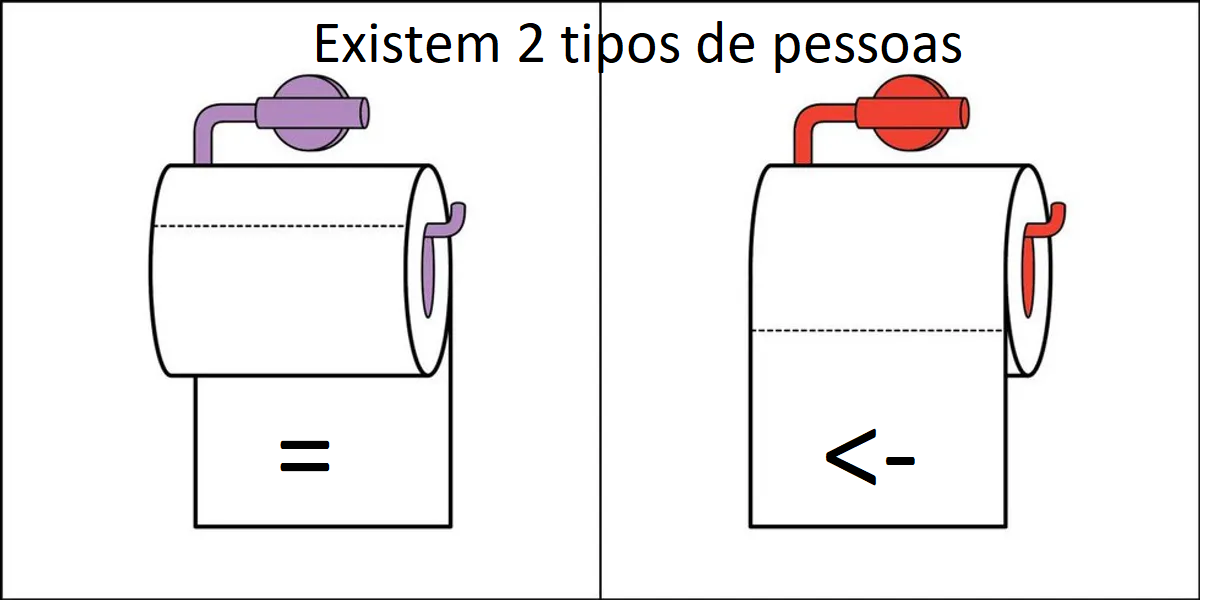
\includegraphics{J:/ENG 792/ENG_792-AVDR/ENG.792-AVDR/Cap_2_2.tipos.de.pessoas.png}
\caption{Existem dois tipos de pessoas: = \& \textless-}
\end{figure}

Com o passar do tempo vamos ``brincando'' com cada operador e, assim, assimilando o que cada uma faz.

\hypertarget{iterauxe7uxf5es}{%
\subsection{Iterações}\label{iterauxe7uxf5es}}

\hypertarget{while}{%
\subsubsection{while()}\label{while}}

Essa forma de \emph{loop} é menos comumente usada e potencialmente perigosa, uma vez que ela pode resultar em uma execução descontrolada. Por isso, em muitos casos iterações restritivas são mais adequadas.
A função \texttt{while()} requer uma condição testável que continuará a resultar em declarações subsequentes a serem executadas até o resultado do teste dar falso (FALSE).

Estrutura:
Começa com a palavra \emph{while} seguida por \emph{parênteses} e \emph{colchetes} \texttt{while()\{\}}
A segunda parte vai dentro de parênteses e diz respeito a uma \emph{expressão lógica} e a terceira parte, entre colchetes, o \emph{corpo do loop}.
\texttt{while(abc)\{xyz\}} \#Se abc for \emph{TRUE} ele vai executar o resto \{xyz\}. Depois volta para checar se (abc) continua \emph{TRUE} ou \emph{FALSE} para decidir se continua no loop ou parar.

\texttt{while(condição)\{}~\\
\texttt{“Código\ a\ ser\ executado”}~\\
\texttt{\}}

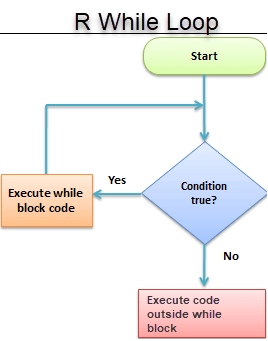
\includegraphics{J:/ENG 792/ENG_792-AVDR/ENG.792-AVDR/Cap_2_while.loop.png}\\
\textbf{Fonte}: \href{https://www.guru99.com/r-while-loop.html}{Guru99}

Exemplo 1: Teste
Ter aula na segunda-feira é bom ou não?

\begin{Shaded}
\begin{Highlighting}[]
\ControlFlowTok{while}\NormalTok{(}\ConstantTok{FALSE}\NormalTok{)\{  }
  \FunctionTok{print}\NormalTok{(}\StringTok{"Aula segunda{-}feira é ótimo!"}\NormalTok{)\}}
\end{Highlighting}
\end{Shaded}

\begin{Shaded}
\begin{Highlighting}[]
\ControlFlowTok{while}\NormalTok{(}\ConstantTok{TRUE}\NormalTok{)\{  }
  \FunctionTok{print}\NormalTok{(}\StringTok{"Aula segunda{-}feira é ótimo!"}\NormalTok{)\}}
\end{Highlighting}
\end{Shaded}

Exemplo 2: Teste
Num concurso de beleza Jackson desafiou qualquer um de seus alunos. Cada um recebeu uma nota.

\begin{Shaded}
\begin{Highlighting}[]
\NormalTok{Jackson}\OtherTok{\textless{}{-}}\FloatTok{9.5}  
\NormalTok{Aluno}\OtherTok{\textless{}{-}}\DecValTok{6}  
\ControlFlowTok{while}\NormalTok{(Aluno}\SpecialCharTok{\textless{}}\NormalTok{Jackson)\{  }
  \FunctionTok{print}\NormalTok{(Jackson)\} }
\end{Highlighting}
\end{Shaded}

\hypertarget{for}{%
\subsubsection{for()}\label{for}}

É similar ao \texttt{while()}, mas é mais conveniente na maioria dos casos.
Iterações restritas (loops) destinam-se a execução de um número fixo de vezes dos comandos usando a função \texttt{for()}.
O loop é executado tantas vezes quanto variam os valores de \emph{i}.
Começa com a palavra \texttt{for} seguindo de por \emph{parênteses} e \emph{colchetes} -- \texttt{for()\{\}}.

\emph{()} não especifica funções lógicas como no while, mas especifica as interações do loop.
\emph{\{\}} são usados para preencher com os comandos do loop

\texttt{for(i\ in\ conjunto\_de\_valores)\{}~\\
\texttt{comandos\ que\ serão\ repetidos}~\\
\texttt{\}}

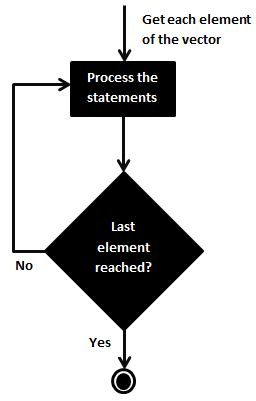
\includegraphics{J:/ENG 792/ENG_792-AVDR/ENG.792-AVDR/Cap_2_for.loop.jpg}\\
\textbf{Fonte:}\href{https://www.tutorialspoint.com/r/r_for_loop.htm}{tutorialspoint}

\begin{Shaded}
\begin{Highlighting}[]
\ControlFlowTok{for}\NormalTok{(i  }\ControlFlowTok{in} \DecValTok{1}\SpecialCharTok{:}\DecValTok{5}\NormalTok{)\{}
  \FunctionTok{print}\NormalTok{(}\StringTok{"Aula segunda{-}feira é ótimo!"}\NormalTok{)}
\NormalTok{\}}
\end{Highlighting}
\end{Shaded}

\begin{verbatim}
## [1] "Aula segunda-feira é ótimo!"
## [1] "Aula segunda-feira é ótimo!"
## [1] "Aula segunda-feira é ótimo!"
## [1] "Aula segunda-feira é ótimo!"
## [1] "Aula segunda-feira é ótimo!"
\end{verbatim}

Significa que \emph{Aula segunda-feira é ótimo!} Será mostrada 5 vezes sempre retornando como o objeto criado \emph{i}.

\begin{Shaded}
\begin{Highlighting}[]
\ControlFlowTok{for}\NormalTok{(i }\ControlFlowTok{in}  \DecValTok{1}\SpecialCharTok{:}\DecValTok{5}\NormalTok{)\{}
  \FunctionTok{print}\NormalTok{((i}\SpecialCharTok{+}\DecValTok{1}\NormalTok{)}\SpecialCharTok{*}\DecValTok{3}\NormalTok{)}
\NormalTok{  \}}
\end{Highlighting}
\end{Shaded}

\begin{verbatim}
## [1] 6
## [1] 9
## [1] 12
## [1] 15
## [1] 18
\end{verbatim}

Não importa onde você começa ou o tipo de vetor que é (\emph{Caractere}, \emph{número} e etc). Basicamente toda vez que mudar ele vai executar o que estiver dentro do corpo do loop.

\hypertarget{condicionais}{%
\subsection{Condicionais}\label{condicionais}}

\hypertarget{if-else}{%
\subsubsection{if, else}\label{if-else}}

A função \texttt{if()} é usado para conduzir uma ou mais declarações contidas dentro de \texttt{{[}{]}}, fornecendo a condição dentro de \texttt{()}.

Voltando para nosso concurso de beleza, temos um controle um pouco mais inteligente do resultado mostrado.

\begin{Shaded}
\begin{Highlighting}[]
\NormalTok{Jackson}\OtherTok{\textless{}{-}}\FloatTok{9.5}  
\NormalTok{Aluno}\OtherTok{\textless{}{-}}\DecValTok{6} 
\ControlFlowTok{if}\NormalTok{(Jackson}\SpecialCharTok{\textgreater{}}\NormalTok{Aluno)\{  }
  \FunctionTok{print}\NormalTok{(}\StringTok{"Jackson é mais bonito que Aluno!"}\NormalTok{)}
\NormalTok{  \}}
\end{Highlighting}
\end{Shaded}

\begin{verbatim}
## [1] "Jackson é mais bonito que Aluno!"
\end{verbatim}

\begin{Shaded}
\begin{Highlighting}[]
\ControlFlowTok{if}\NormalTok{(Aluno}\SpecialCharTok{*}\DecValTok{2}\SpecialCharTok{\textgreater{}=}\NormalTok{Jackson)\{}
  \FunctionTok{print}\NormalTok{(}\StringTok{"Aluno é mais bonito!"}\NormalTok{)}
\NormalTok{  \}}
\end{Highlighting}
\end{Shaded}

\begin{verbatim}
## [1] "Aluno é mais bonito!"
\end{verbatim}

Adaptando a o código acima para fazer a declaração condicional \textbf{FALSE} simplesmente retorna nenhum comando no prompt uma vez que o código não disse como \textbf{R} deveria responder nesse caso.

\begin{Shaded}
\begin{Highlighting}[]
\ControlFlowTok{if}\NormalTok{(Aluno}\SpecialCharTok{*}\DecValTok{2}\SpecialCharTok{\textgreater{}=}\NormalTok{Jackson}\SpecialCharTok{\^{}}\DecValTok{2}\NormalTok{)\{}
    \FunctionTok{print}\NormalTok{(}\StringTok{"Aluno é mais bonito!"}\NormalTok{)}
\NormalTok{  \}}
\end{Highlighting}
\end{Shaded}

Existem 2 métodos de informar ao R como responder em casos onde a declaração de condição é retornada como \textbf{FALSE}: usando o modificador \texttt{else} ou a função \texttt{ifelse()}.
Ao contrário de uma função qualquer, \texttt{else} não pode ser usado independentemente, mas apenas como um modificador (adição) ao \texttt{if()}. \texttt{If} no exemplo acima, o resultado é solicitado quando o valor retornado é \textbf{FALSE}, \texttt{else} pode ser adicionado como segue:

\begin{Shaded}
\begin{Highlighting}[]
\ControlFlowTok{if}\NormalTok{(Aluno}\SpecialCharTok{*}\DecValTok{2}\SpecialCharTok{\textgreater{}=}\NormalTok{Jackson}\SpecialCharTok{\^{}}\DecValTok{2}\NormalTok{)\{}
    \FunctionTok{print}\NormalTok{(}\StringTok{"A declaração é verdadeira!"}\NormalTok{)}
\NormalTok{  \}}\ControlFlowTok{else}\NormalTok{\{}
    \FunctionTok{print}\NormalTok{(}\StringTok{"A declaração é falsa!"}\NormalTok{)}
\NormalTok{    \}}
\end{Highlighting}
\end{Shaded}

\begin{verbatim}
## [1] "A declaração é falsa!"
\end{verbatim}

Note que \texttt{else} foi escrito na mesma linha que conclui o \texttt{if()} para informar ao R que o teste condicional continua.

Podemos retirar a segunda parte do teste anterior e adicionar uma nova comparação.

\begin{Shaded}
\begin{Highlighting}[]
\NormalTok{Aluno2}\OtherTok{\textless{}{-}}\DecValTok{7}
\ControlFlowTok{if}\NormalTok{(Aluno2}\SpecialCharTok{\textgreater{}}\NormalTok{Jackson)\{}
    \FunctionTok{print}\NormalTok{(}\StringTok{"Aluno1 é mais bonito!"}\NormalTok{)}
\NormalTok{  \}}\ControlFlowTok{else} \ControlFlowTok{if}\NormalTok{(Aluno2}\SpecialCharTok{\textgreater{}}\NormalTok{Aluno)\{}
    \FunctionTok{print}\NormalTok{(}\StringTok{"Aluno2 é mais bonito que Aluno e menos bonito que Jackson."}\NormalTok{)}
\NormalTok{    \}}
\end{Highlighting}
\end{Shaded}

\begin{verbatim}
## [1] "Aluno2 é mais bonito que Aluno e menos bonito que Jackson."
\end{verbatim}

\hypertarget{ifelse}{%
\subsubsection{ifelse()}\label{ifelse}}

A função \texttt{ifelse()} é separada de \texttt{if()} e é formada de uma sintaxe mais simples e concisa. No entanto, ela pode ser usada para gerar o mesmo efeito que nas demonstrações anteriores usando \texttt{if()} com o modificador \texttt{else}.

\begin{Shaded}
\begin{Highlighting}[]
\FunctionTok{ifelse}\NormalTok{(Aluno}\SpecialCharTok{*}\DecValTok{2}\SpecialCharTok{\textgreater{}=}\NormalTok{Jackson}\SpecialCharTok{\^{}}\DecValTok{2}\NormalTok{, }\StringTok{"Aluno é mais bonito!"}\NormalTok{, }\StringTok{"Jackson é mais bonito!"}\NormalTok{)}
\end{Highlighting}
\end{Shaded}

\begin{verbatim}
## [1] "Jackson é mais bonito!"
\end{verbatim}

Como mostrado acima, o uso de \texttt{ifelse()} usa a forma:
\texttt{ifelse(teste\ condicional,\ resultado\ se\ verdadeiro,\ resultado\ se\ falso)}

Declarações condicionais também podem ser aninhadas dentro uma outra. Adaptando o exemplo com o argumento \texttt{else} um outro teste é executado se o teste inicial é \textbf{FALSE}, onde o secundário é \textbf{TRUE}.

\begin{Shaded}
\begin{Highlighting}[]
\FunctionTok{ifelse}\NormalTok{(Aluno}\SpecialCharTok{*}\DecValTok{2}\SpecialCharTok{\textgreater{}=}\NormalTok{Jackson}\SpecialCharTok{\^{}}\DecValTok{2}\NormalTok{, }\StringTok{"Aluno é mais bonito!"}\NormalTok{,}
       \FunctionTok{ifelse}\NormalTok{(Aluno}\SpecialCharTok{*}\DecValTok{2}\SpecialCharTok{\textgreater{}=}\NormalTok{Jackson}\SpecialCharTok{\^{}}\FloatTok{0.5}\NormalTok{ ,}\StringTok{"Agora o Aluno é mais bonito!"}\NormalTok{, }\StringTok{"Aluno continua feio!"}\NormalTok{))}
\end{Highlighting}
\end{Shaded}

\begin{verbatim}
## [1] "Agora o Aluno é mais bonito!"
\end{verbatim}

Se o teste secundário é ajustado de maneira que os resultados em um teste lógico \textbf{FALSE}, o seguinte resultado é retornado.

\begin{Shaded}
\begin{Highlighting}[]
\FunctionTok{ifelse}\NormalTok{(Aluno}\SpecialCharTok{*}\DecValTok{2}\SpecialCharTok{\textgreater{}=}\NormalTok{Jackson}\SpecialCharTok{\^{}}\DecValTok{2}\NormalTok{, }\StringTok{"Aluno é mais bonito!"}\NormalTok{,}
       \FunctionTok{ifelse}\NormalTok{(Aluno}\SpecialCharTok{*}\DecValTok{2}\SpecialCharTok{\textgreater{}=}\NormalTok{Jackson}\SpecialCharTok{\^{}}\DecValTok{3}\NormalTok{,}\StringTok{"Agora o Aluno é mais bonito!"}\NormalTok{, }\StringTok{"Aluno continua feio!"}\NormalTok{))}
\end{Highlighting}
\end{Shaded}

\begin{verbatim}
## [1] "Aluno continua feio!"
\end{verbatim}

\hypertarget{dica-de-leitura}{%
\section{Dica de leitura}\label{dica-de-leitura}}

\href{https://rspatial.org/intr/4-indexing.html}{Spatial Data Science - Indexing}

\href{http://www.cookbook-r.com/Basics/Indexing_into_a_data_structure/}{Indexing into a data structure}\\
\href{https://www.datamentor.io/r-programming/if-else-statement/}{datamentor - R if\ldots else Statement}

\hypertarget{exercuxedcios}{%
\section{Exercícios}\label{exercuxedcios}}

\begin{enumerate}
\def\labelenumi{\arabic{enumi}.}
\tightlist
\item
  Crie o vetor \emph{p} que contenham uma sequência de \emph{200} iniciando em \emph{0} aumentando \emph{0.5}.
\item
  Eleve o vetor \emph{p} ao cubo criando o vetor \emph{o} e multiplique por \emph{p}.
  Organize \emph{p} por linhas em uma matriz com 10 colunas .\\
\item
  Crie os elementos \texttt{x\ \ =\ 10} e \texttt{y\ =\ 25}.
\item
  Mostre na tela \textbf{A declaração é verdadeira} sob a condição de \emph{x} ser menor que \emph{y}.
\item
  Mostre 2 maneiras condicionais de executar a declaração na qual mostraria \textbf{A declaração é correta} se \emph{x} é menor ou igual a \emph{y}, ou caso contrário mostre \textbf{A declaração é incorreta} se não for o caso.
\item
  Atribua \texttt{z\ =\ 50} e construa uma função \texttt{ifelse()} que testa se \emph{x} é maior que \emph{y}, mostrando \textbf{true} se a condição é encontrada. Aninhe dentro disso uma segunda condição que mostre \textbf{uma verdadeira, uma falsa} ou \textbf{ambas falsas} caso \emph{x} seja maior que \emph{z}.
\item
  Use uma iteração restrita para gerar uma sequência de números de 1 até 20.
\item
  Use iteração restrita para conduzir o cálculo \texttt{(i\^{}2)-i}, onde \emph{i} vai de 5 até 10.
\item
  Use interação não restrita para gerar uma sequência de inteiros de -10 até -20.
\end{enumerate}

  \bibliography{book.bib,packages.bib}

\end{document}
